\documentclass[]{article}
\usepackage{lmodern}
\usepackage{amssymb,amsmath}
\usepackage{ifxetex,ifluatex}
\usepackage{fixltx2e} % provides \textsubscript
\ifnum 0\ifxetex 1\fi\ifluatex 1\fi=0 % if pdftex
  \usepackage[T1]{fontenc}
  \usepackage[utf8]{inputenc}
\else % if luatex or xelatex
  \ifxetex
    \usepackage{mathspec}
  \else
    \usepackage{fontspec}
  \fi
  \defaultfontfeatures{Ligatures=TeX,Scale=MatchLowercase}
\fi
% use upquote if available, for straight quotes in verbatim environments
\IfFileExists{upquote.sty}{\usepackage{upquote}}{}
% use microtype if available
\IfFileExists{microtype.sty}{%
\usepackage{microtype}
\UseMicrotypeSet[protrusion]{basicmath} % disable protrusion for tt fonts
}{}
\usepackage[margin=1in]{geometry}
\usepackage{hyperref}
\hypersetup{unicode=true,
            pdftitle={codigoTFG},
            pdfauthor={Jorge de Andrés},
            pdfborder={0 0 0},
            breaklinks=true}
\urlstyle{same}  % don't use monospace font for urls
\usepackage{color}
\usepackage{fancyvrb}
\newcommand{\VerbBar}{|}
\newcommand{\VERB}{\Verb[commandchars=\\\{\}]}
\DefineVerbatimEnvironment{Highlighting}{Verbatim}{commandchars=\\\{\}}
% Add ',fontsize=\small' for more characters per line
\usepackage{framed}
\definecolor{shadecolor}{RGB}{248,248,248}
\newenvironment{Shaded}{\begin{snugshade}}{\end{snugshade}}
\newcommand{\KeywordTok}[1]{\textcolor[rgb]{0.13,0.29,0.53}{\textbf{#1}}}
\newcommand{\DataTypeTok}[1]{\textcolor[rgb]{0.13,0.29,0.53}{#1}}
\newcommand{\DecValTok}[1]{\textcolor[rgb]{0.00,0.00,0.81}{#1}}
\newcommand{\BaseNTok}[1]{\textcolor[rgb]{0.00,0.00,0.81}{#1}}
\newcommand{\FloatTok}[1]{\textcolor[rgb]{0.00,0.00,0.81}{#1}}
\newcommand{\ConstantTok}[1]{\textcolor[rgb]{0.00,0.00,0.00}{#1}}
\newcommand{\CharTok}[1]{\textcolor[rgb]{0.31,0.60,0.02}{#1}}
\newcommand{\SpecialCharTok}[1]{\textcolor[rgb]{0.00,0.00,0.00}{#1}}
\newcommand{\StringTok}[1]{\textcolor[rgb]{0.31,0.60,0.02}{#1}}
\newcommand{\VerbatimStringTok}[1]{\textcolor[rgb]{0.31,0.60,0.02}{#1}}
\newcommand{\SpecialStringTok}[1]{\textcolor[rgb]{0.31,0.60,0.02}{#1}}
\newcommand{\ImportTok}[1]{#1}
\newcommand{\CommentTok}[1]{\textcolor[rgb]{0.56,0.35,0.01}{\textit{#1}}}
\newcommand{\DocumentationTok}[1]{\textcolor[rgb]{0.56,0.35,0.01}{\textbf{\textit{#1}}}}
\newcommand{\AnnotationTok}[1]{\textcolor[rgb]{0.56,0.35,0.01}{\textbf{\textit{#1}}}}
\newcommand{\CommentVarTok}[1]{\textcolor[rgb]{0.56,0.35,0.01}{\textbf{\textit{#1}}}}
\newcommand{\OtherTok}[1]{\textcolor[rgb]{0.56,0.35,0.01}{#1}}
\newcommand{\FunctionTok}[1]{\textcolor[rgb]{0.00,0.00,0.00}{#1}}
\newcommand{\VariableTok}[1]{\textcolor[rgb]{0.00,0.00,0.00}{#1}}
\newcommand{\ControlFlowTok}[1]{\textcolor[rgb]{0.13,0.29,0.53}{\textbf{#1}}}
\newcommand{\OperatorTok}[1]{\textcolor[rgb]{0.81,0.36,0.00}{\textbf{#1}}}
\newcommand{\BuiltInTok}[1]{#1}
\newcommand{\ExtensionTok}[1]{#1}
\newcommand{\PreprocessorTok}[1]{\textcolor[rgb]{0.56,0.35,0.01}{\textit{#1}}}
\newcommand{\AttributeTok}[1]{\textcolor[rgb]{0.77,0.63,0.00}{#1}}
\newcommand{\RegionMarkerTok}[1]{#1}
\newcommand{\InformationTok}[1]{\textcolor[rgb]{0.56,0.35,0.01}{\textbf{\textit{#1}}}}
\newcommand{\WarningTok}[1]{\textcolor[rgb]{0.56,0.35,0.01}{\textbf{\textit{#1}}}}
\newcommand{\AlertTok}[1]{\textcolor[rgb]{0.94,0.16,0.16}{#1}}
\newcommand{\ErrorTok}[1]{\textcolor[rgb]{0.64,0.00,0.00}{\textbf{#1}}}
\newcommand{\NormalTok}[1]{#1}
\usepackage{graphicx,grffile}
\makeatletter
\def\maxwidth{\ifdim\Gin@nat@width>\linewidth\linewidth\else\Gin@nat@width\fi}
\def\maxheight{\ifdim\Gin@nat@height>\textheight\textheight\else\Gin@nat@height\fi}
\makeatother
% Scale images if necessary, so that they will not overflow the page
% margins by default, and it is still possible to overwrite the defaults
% using explicit options in \includegraphics[width, height, ...]{}
\setkeys{Gin}{width=\maxwidth,height=\maxheight,keepaspectratio}
\IfFileExists{parskip.sty}{%
\usepackage{parskip}
}{% else
\setlength{\parindent}{0pt}
\setlength{\parskip}{6pt plus 2pt minus 1pt}
}
\setlength{\emergencystretch}{3em}  % prevent overfull lines
\providecommand{\tightlist}{%
  \setlength{\itemsep}{0pt}\setlength{\parskip}{0pt}}
\setcounter{secnumdepth}{0}
% Redefines (sub)paragraphs to behave more like sections
\ifx\paragraph\undefined\else
\let\oldparagraph\paragraph
\renewcommand{\paragraph}[1]{\oldparagraph{#1}\mbox{}}
\fi
\ifx\subparagraph\undefined\else
\let\oldsubparagraph\subparagraph
\renewcommand{\subparagraph}[1]{\oldsubparagraph{#1}\mbox{}}
\fi

%%% Use protect on footnotes to avoid problems with footnotes in titles
\let\rmarkdownfootnote\footnote%
\def\footnote{\protect\rmarkdownfootnote}

%%% Change title format to be more compact
\usepackage{titling}

% Create subtitle command for use in maketitle
\newcommand{\subtitle}[1]{
  \posttitle{
    \begin{center}\large#1\end{center}
    }
}

\setlength{\droptitle}{-2em}

  \title{codigoTFG}
    \pretitle{\vspace{\droptitle}\centering\huge}
  \posttitle{\par}
    \author{Jorge de Andrés}
    \preauthor{\centering\large\emph}
  \postauthor{\par}
      \predate{\centering\large\emph}
  \postdate{\par}
    \date{12 de enero de 2019}


\begin{document}
\maketitle

Borramos el environment lo primero para siempre tenerlo limpio en la
ejecución:

\begin{Shaded}
\begin{Highlighting}[]
\KeywordTok{rm}\NormalTok{(}\DataTypeTok{list=}\KeywordTok{ls}\NormalTok{())}
\end{Highlighting}
\end{Shaded}

Importamos todas las librerías que vamos a ir necesitando:

\begin{Shaded}
\begin{Highlighting}[]
\CommentTok{#install.packages("ggplot2")}
\CommentTok{#install.packages("caret")}
\CommentTok{#install.packages("plyr")}
\CommentTok{#install.packages("wordcloud")}
\CommentTok{#install.packages("hexbin")}
\CommentTok{#install.packages("RColorBrewer")}
\CommentTok{#install.packages("corrplot")}
\CommentTok{#install.packages("FactoMineR")}
\CommentTok{#devtools::install_github("kassambara/factoextra")}
\CommentTok{#install.packages("factoextra")}
\CommentTok{#install.packages("nnet")}
\CommentTok{#install.packages("plotly")}
\CommentTok{#install.packages("class")}
\CommentTok{#install.packages("gmodels")}
\CommentTok{#install.packages("randomForest")}
\CommentTok{#install.packages("e1071")}
\CommentTok{#install.packages("ape")}
\CommentTok{#install.packages("cluster")}
\CommentTok{#install.packages("fpc")}
\CommentTok{#install.packages("RWeka")}

\KeywordTok{library}\NormalTok{(}\StringTok{"ggplot2"}\NormalTok{)}
\KeywordTok{library}\NormalTok{(}\StringTok{"caret"}\NormalTok{)}
\end{Highlighting}
\end{Shaded}

\begin{verbatim}
## Loading required package: lattice
\end{verbatim}

\begin{Shaded}
\begin{Highlighting}[]
\KeywordTok{library}\NormalTok{(}\StringTok{"plyr"}\NormalTok{)}
\KeywordTok{library}\NormalTok{(}\StringTok{"wordcloud"}\NormalTok{)}
\end{Highlighting}
\end{Shaded}

\begin{verbatim}
## Loading required package: RColorBrewer
\end{verbatim}

\begin{Shaded}
\begin{Highlighting}[]
\KeywordTok{library}\NormalTok{(}\StringTok{"hexbin"}\NormalTok{)}
\KeywordTok{library}\NormalTok{(}\StringTok{"RColorBrewer"}\NormalTok{)}
\KeywordTok{library}\NormalTok{(}\StringTok{"corrplot"}\NormalTok{)}
\end{Highlighting}
\end{Shaded}

\begin{verbatim}
## corrplot 0.84 loaded
\end{verbatim}

\begin{Shaded}
\begin{Highlighting}[]
\KeywordTok{library}\NormalTok{(}\StringTok{"FactoMineR"}\NormalTok{)}
\KeywordTok{library}\NormalTok{(}\StringTok{"factoextra"}\NormalTok{)}
\end{Highlighting}
\end{Shaded}

\begin{verbatim}
## Welcome! Related Books: `Practical Guide To Cluster Analysis in R` at https://goo.gl/13EFCZ
\end{verbatim}

\begin{Shaded}
\begin{Highlighting}[]
\KeywordTok{library}\NormalTok{(}\StringTok{"nnet"}\NormalTok{)}
\KeywordTok{library}\NormalTok{(}\StringTok{"plotly"}\NormalTok{)}
\end{Highlighting}
\end{Shaded}

\begin{verbatim}
## 
## Attaching package: 'plotly'
\end{verbatim}

\begin{verbatim}
## The following objects are masked from 'package:plyr':
## 
##     arrange, mutate, rename, summarise
\end{verbatim}

\begin{verbatim}
## The following object is masked from 'package:ggplot2':
## 
##     last_plot
\end{verbatim}

\begin{verbatim}
## The following object is masked from 'package:stats':
## 
##     filter
\end{verbatim}

\begin{verbatim}
## The following object is masked from 'package:graphics':
## 
##     layout
\end{verbatim}

\begin{Shaded}
\begin{Highlighting}[]
\KeywordTok{library}\NormalTok{(}\StringTok{"class"}\NormalTok{)}
\KeywordTok{library}\NormalTok{(}\StringTok{"gmodels"}\NormalTok{)}
\KeywordTok{library}\NormalTok{(}\StringTok{"randomForest"}\NormalTok{)}
\end{Highlighting}
\end{Shaded}

\begin{verbatim}
## randomForest 4.6-14
\end{verbatim}

\begin{verbatim}
## Type rfNews() to see new features/changes/bug fixes.
\end{verbatim}

\begin{verbatim}
## 
## Attaching package: 'randomForest'
\end{verbatim}

\begin{verbatim}
## The following object is masked from 'package:ggplot2':
## 
##     margin
\end{verbatim}

\begin{Shaded}
\begin{Highlighting}[]
\KeywordTok{library}\NormalTok{(}\StringTok{"e1071"}\NormalTok{)}
\KeywordTok{library}\NormalTok{(}\StringTok{"ape"}\NormalTok{)}
\KeywordTok{library}\NormalTok{(}\StringTok{"cluster"}\NormalTok{)}
\KeywordTok{library}\NormalTok{(}\StringTok{"fpc"}\NormalTok{)}
\KeywordTok{library}\NormalTok{(}\StringTok{"RWeka"}\NormalTok{)}
\end{Highlighting}
\end{Shaded}

Lo primero que tengo que hacer es importar el dataset que he creado:

\begin{Shaded}
\begin{Highlighting}[]
\NormalTok{dataset <-}\StringTok{ }\KeywordTok{read.csv}\NormalTok{(}\StringTok{"Datos/datos.txt"}\NormalTok{, }\DataTypeTok{header =} \OtherTok{TRUE}\NormalTok{)}
\end{Highlighting}
\end{Shaded}

Ahora lo que hago es pasarlo a una matriz, quitando tanto el nombre (que
no me interesa) como la etiqueta (que no la necesito por ahora):

\begin{Shaded}
\begin{Highlighting}[]
\NormalTok{matriz.pacientes.etiquetas <-}\StringTok{ }\NormalTok{dataset[, }\OperatorTok{-}\DecValTok{1}\NormalTok{]}
\NormalTok{matriz.pacientes.datos <-}\StringTok{ }\NormalTok{matriz.pacientes.etiquetas[, }\OperatorTok{-}\DecValTok{25}\NormalTok{]}
\end{Highlighting}
\end{Shaded}

\section{Análisis Exploratorio}\label{analisis-exploratorio}

Primero compruebo que todos los datos tienen un tipo correcto.

\begin{Shaded}
\begin{Highlighting}[]
\KeywordTok{sapply}\NormalTok{(matriz.pacientes.datos, class)}
\end{Highlighting}
\end{Shaded}

\begin{verbatim}
##              edad               sex rel_ctxo_rel_mala   rel_ctxo_trauma 
##         "integer"         "integer"         "integer"         "integer" 
##    rel_ctxo_buena           ed_perm           ed_norm           ed_estr 
##         "integer"         "integer"         "integer"         "integer" 
##          resil_ba          resil_me          resil_al           pen_dic 
##         "integer"         "integer"         "integer"         "integer" 
##            gen_ex              etiq           fil_men           max_min 
##         "integer"         "integer"         "integer"         "integer" 
##          conc_arb          pseu_res               deb           raz_emo 
##         "integer"         "integer"         "integer"         "integer" 
##             inhib             asert             agres            impuls 
##         "integer"         "integer"         "integer"         "integer"
\end{verbatim}

Veo la media de la edad de los pacientes y el rango en el que se mueve

\begin{Shaded}
\begin{Highlighting}[]
\KeywordTok{mean}\NormalTok{(matriz.pacientes.datos[, }\DecValTok{1}\NormalTok{])}
\end{Highlighting}
\end{Shaded}

\begin{verbatim}
## [1] 26.46269
\end{verbatim}

\begin{Shaded}
\begin{Highlighting}[]
\KeywordTok{range}\NormalTok{(matriz.pacientes.datos[, }\DecValTok{1}\NormalTok{])}
\end{Highlighting}
\end{Shaded}

\begin{verbatim}
## [1] 13 52
\end{verbatim}

Voy a ver estos datos gráficamente:

\begin{Shaded}
\begin{Highlighting}[]
\KeywordTok{qplot}\NormalTok{(}\DecValTok{1}\NormalTok{, matriz.pacientes.datos[, }\DecValTok{1}\NormalTok{], }\DataTypeTok{xlab =} \StringTok{"Pacientes"}\NormalTok{, }\DataTypeTok{ylab =} \StringTok{"Edad"}\NormalTok{, }\DataTypeTok{geom=}\StringTok{"boxplot"}\NormalTok{)}
\end{Highlighting}
\end{Shaded}

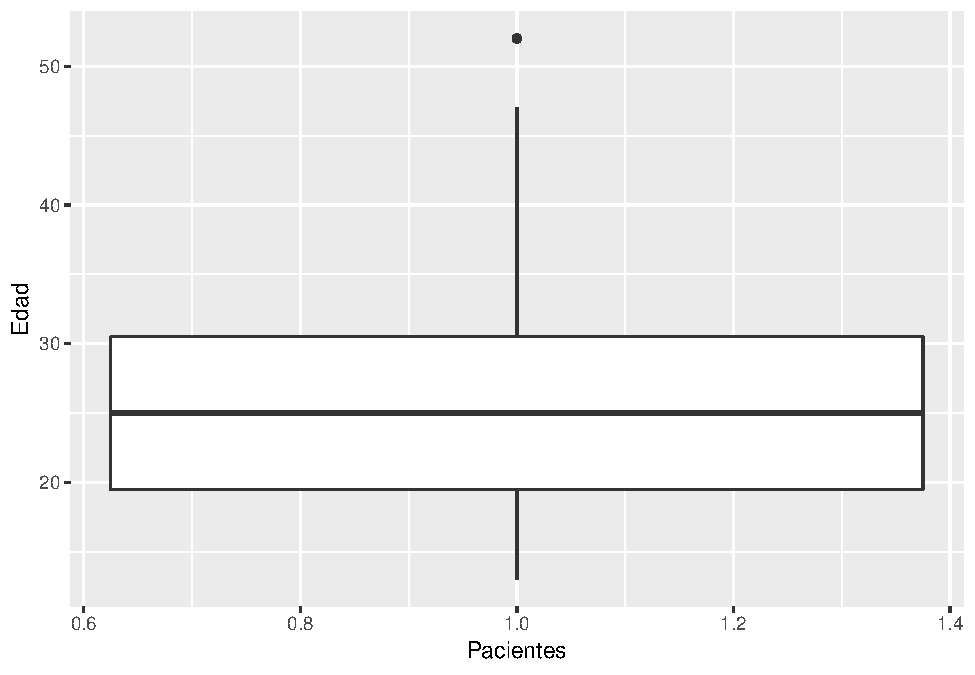
\includegraphics{codigo_files/figure-latex/grafico_estadistica_edad-1.pdf}
Pasamos el qplot a PDF:

\begin{Shaded}
\begin{Highlighting}[]
\KeywordTok{pdf}\NormalTok{(}\StringTok{"Imágenes Obtenidas/boxplotEdadPacientes.pdf"}\NormalTok{)}

\KeywordTok{qplot}\NormalTok{(}\DecValTok{1}\NormalTok{, matriz.pacientes.datos[, }\DecValTok{1}\NormalTok{], }\DataTypeTok{xlab =} \StringTok{"Pacientes"}\NormalTok{, }\DataTypeTok{ylab =} \StringTok{"Edad"}\NormalTok{, }\DataTypeTok{geom=}\StringTok{"boxplot"}\NormalTok{)}

\NormalTok{dev.off}
\end{Highlighting}
\end{Shaded}

\begin{verbatim}
## function (which = dev.cur()) 
## {
##     if (which == 1) 
##         stop("cannot shut down device 1 (the null device)")
##     .External(C_devoff, as.integer(which))
##     dev.cur()
## }
## <bytecode: 0x0000000015754360>
## <environment: namespace:grDevices>
\end{verbatim}

Finalmente, veo un resúmen de cada columna

\begin{Shaded}
\begin{Highlighting}[]
\KeywordTok{summary}\NormalTok{(matriz.pacientes.datos)}
\end{Highlighting}
\end{Shaded}

\begin{verbatim}
##       edad            sex        rel_ctxo_rel_mala rel_ctxo_trauma 
##  Min.   :13.00   Min.   :0.000   Min.   :0.0000    Min.   :0.0000  
##  1st Qu.:19.50   1st Qu.:0.000   1st Qu.:0.0000    1st Qu.:0.0000  
##  Median :25.00   Median :0.000   Median :0.0000    Median :0.0000  
##  Mean   :26.46   Mean   :0.209   Mean   :0.1343    Mean   :0.3582  
##  3rd Qu.:30.50   3rd Qu.:0.000   3rd Qu.:0.0000    3rd Qu.:1.0000  
##  Max.   :52.00   Max.   :1.000   Max.   :1.0000    Max.   :1.0000  
##  rel_ctxo_buena      ed_perm          ed_norm          ed_estr      
##  Min.   :0.0000   Min.   :0.0000   Min.   :0.0000   Min.   :0.0000  
##  1st Qu.:0.0000   1st Qu.:0.0000   1st Qu.:0.0000   1st Qu.:0.0000  
##  Median :1.0000   Median :0.0000   Median :0.0000   Median :0.0000  
##  Mean   :0.5075   Mean   :0.2836   Mean   :0.4925   Mean   :0.2239  
##  3rd Qu.:1.0000   3rd Qu.:1.0000   3rd Qu.:1.0000   3rd Qu.:0.0000  
##  Max.   :1.0000   Max.   :1.0000   Max.   :1.0000   Max.   :1.0000  
##     resil_ba         resil_me         resil_al          pen_dic      
##  Min.   :0.0000   Min.   :0.0000   Min.   :0.00000   Min.   :0.0000  
##  1st Qu.:0.0000   1st Qu.:0.0000   1st Qu.:0.00000   1st Qu.:1.0000  
##  Median :1.0000   Median :0.0000   Median :0.00000   Median :1.0000  
##  Mean   :0.5672   Mean   :0.4179   Mean   :0.01493   Mean   :0.8955  
##  3rd Qu.:1.0000   3rd Qu.:1.0000   3rd Qu.:0.00000   3rd Qu.:1.0000  
##  Max.   :1.0000   Max.   :1.0000   Max.   :1.00000   Max.   :1.0000  
##      gen_ex            etiq           fil_men         max_min      
##  Min.   :0.0000   Min.   :0.0000   Min.   :0.000   Min.   :0.0000  
##  1st Qu.:1.0000   1st Qu.:0.5000   1st Qu.:1.000   1st Qu.:1.0000  
##  Median :1.0000   Median :1.0000   Median :1.000   Median :1.0000  
##  Mean   :0.9552   Mean   :0.7463   Mean   :0.791   Mean   :0.9701  
##  3rd Qu.:1.0000   3rd Qu.:1.0000   3rd Qu.:1.000   3rd Qu.:1.0000  
##  Max.   :1.0000   Max.   :1.0000   Max.   :1.000   Max.   :1.0000  
##     conc_arb         pseu_res           deb            raz_emo     
##  Min.   :0.0000   Min.   :0.0000   Min.   :0.0000   Min.   :0.000  
##  1st Qu.:1.0000   1st Qu.:0.0000   1st Qu.:1.0000   1st Qu.:1.000  
##  Median :1.0000   Median :1.0000   Median :1.0000   Median :1.000  
##  Mean   :0.9851   Mean   :0.5075   Mean   :0.9403   Mean   :0.791  
##  3rd Qu.:1.0000   3rd Qu.:1.0000   3rd Qu.:1.0000   3rd Qu.:1.000  
##  Max.   :1.0000   Max.   :1.0000   Max.   :1.0000   Max.   :1.000  
##      inhib            asert            agres           impuls      
##  Min.   :0.0000   Min.   :0.0000   Min.   :0.000   Min.   :0.0000  
##  1st Qu.:0.0000   1st Qu.:0.0000   1st Qu.:0.000   1st Qu.:0.0000  
##  Median :1.0000   Median :0.0000   Median :0.000   Median :1.0000  
##  Mean   :0.6567   Mean   :0.1343   Mean   :0.209   Mean   :0.6119  
##  3rd Qu.:1.0000   3rd Qu.:0.0000   3rd Qu.:0.000   3rd Qu.:1.0000  
##  Max.   :1.0000   Max.   :1.0000   Max.   :1.000   Max.   :1.0000
\end{verbatim}

Como se puede ver, los datos de los pacientes están muy distanciados, y
además su media es muy alta. Así, la media de la edad difiere
enormemente del resto de valores de la matriz. Debido a ello, debemos de
hacer un preprocesado de los datos del problema.

\section{Preparación de los datos}\label{preparacion-de-los-datos}

Como he comentado antes, Lo que voy a hacer ahora es un centrado y
escalado de los datos de la matriz. De esta manera, la red neuronal no
tendrá ningún valor que destaque especialmente y con ello no dará de
inicio más peso a unos valores que a otros, ya que no lo buscamos.

Ahora hacemos un centrado y escalado de los datos, ya que la edad no
sigue el rango del resto de valores, y distorsionaría la predicción

\begin{Shaded}
\begin{Highlighting}[]
\NormalTok{preObjeto <-}\StringTok{ }\KeywordTok{preProcess}\NormalTok{(matriz.pacientes.datos, }\DataTypeTok{method=}\KeywordTok{c}\NormalTok{(}\StringTok{"center"}\NormalTok{, }\StringTok{"scale"}\NormalTok{))  }\CommentTok{# Quiero hacer un centrado y escalado}
\NormalTok{matriz.pacientes.datos.centscal <-}\StringTok{ }\KeywordTok{predict}\NormalTok{(preObjeto, matriz.pacientes.datos) }\CommentTok{# Obtengo los valores en la matriz centscal}
\end{Highlighting}
\end{Shaded}

Después del preprocesado, aunque con los datos no preprocesados, voy a
hacer la visualización de algunas relaciones entre variables, de tal
manera que podamos ver gráficamente algunos aspectos interesantes:

\subsection{Visualización de Datos}\label{visualizacion-de-datos}

Para empezar voy a sacar una nube de palabras para mostrar los nombres
más comúnes en los datos facilitados:

\begin{Shaded}
\begin{Highlighting}[]
\CommentTok{# Lo primero que tengo que hacer es contar la frecuencia de los nombres}

\NormalTok{dataNombres <-}\StringTok{ }\KeywordTok{ddply}\NormalTok{(dataset,.(nom),nrow)}
\NormalTok{dataNombres <-}\StringTok{ }\NormalTok{dataNombres[}\KeywordTok{order}\NormalTok{(dataNombres}\OperatorTok{$}\NormalTok{V1, }\DataTypeTok{decreasing =} \OtherTok{TRUE}\NormalTok{), ]}
\end{Highlighting}
\end{Shaded}

Una vez que tengo los nombres contados y ordenados, es el momento de
crear la WordCloud

\begin{Shaded}
\begin{Highlighting}[]
\KeywordTok{set.seed}\NormalTok{(}\DecValTok{9999}\NormalTok{) }\CommentTok{# Para el mantenimiento del mismo patrón}

\KeywordTok{wordcloud}\NormalTok{(}\DataTypeTok{words =}\NormalTok{ dataNombres}\OperatorTok{$}\NormalTok{nom, }\DataTypeTok{freq =}\NormalTok{ dataNombres}\OperatorTok{$}\NormalTok{V1, }\DataTypeTok{min.freq =} \DecValTok{1}\NormalTok{, }\DataTypeTok{random.order=}\OtherTok{FALSE}\NormalTok{, }\DataTypeTok{rot.per=}\FloatTok{0.5}\NormalTok{, }\DataTypeTok{colors=}\KeywordTok{c}\NormalTok{(}\StringTok{"Orange"}\NormalTok{,}\StringTok{"Purple"}\NormalTok{,}\StringTok{"Pink"}\NormalTok{, }\StringTok{"Red"}\NormalTok{, }\StringTok{"Yellow"}\NormalTok{, }\StringTok{"Green"}\NormalTok{, }\StringTok{"Blue"}\NormalTok{, }\StringTok{"Black"}\NormalTok{))}
\end{Highlighting}
\end{Shaded}

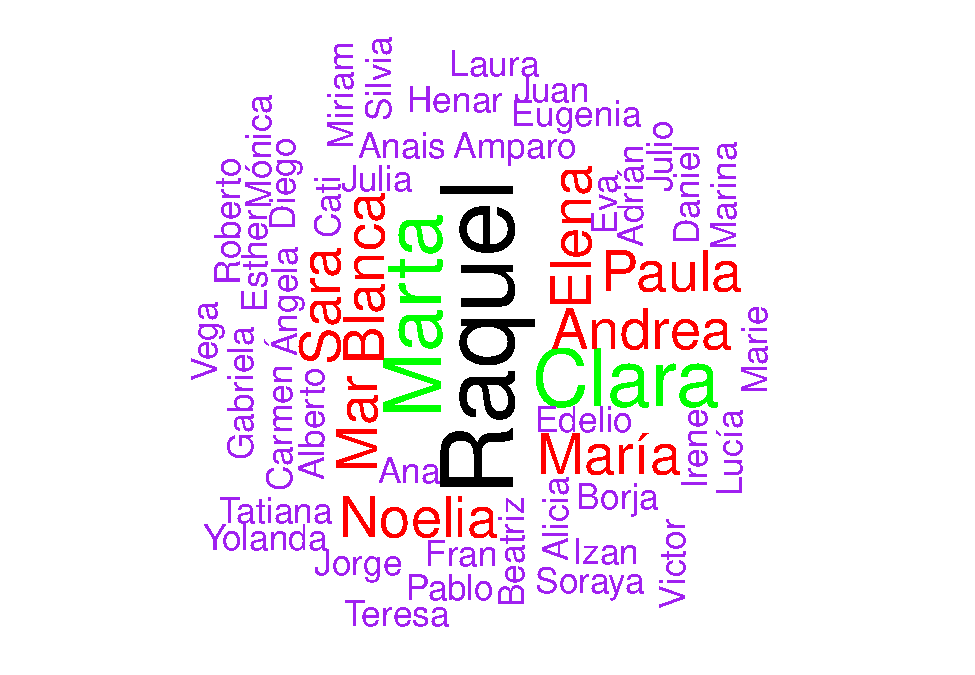
\includegraphics{codigo_files/figure-latex/wordcloud-1.pdf}

Lo pasamos a PDF:

\begin{Shaded}
\begin{Highlighting}[]
\KeywordTok{set.seed}\NormalTok{(}\DecValTok{9999}\NormalTok{)}

\KeywordTok{pdf}\NormalTok{(}\StringTok{"Imágenes Obtenidas/wordcloudNombresPacientes.pdf"}\NormalTok{)}

\KeywordTok{wordcloud}\NormalTok{(}\DataTypeTok{words =}\NormalTok{ dataNombres}\OperatorTok{$}\NormalTok{nom, }\DataTypeTok{freq =}\NormalTok{ dataNombres}\OperatorTok{$}\NormalTok{V1, }\DataTypeTok{min.freq =} \DecValTok{1}\NormalTok{, }\DataTypeTok{random.order=}\OtherTok{FALSE}\NormalTok{, }\DataTypeTok{rot.per=}\FloatTok{0.5}\NormalTok{, }\DataTypeTok{colors=}\KeywordTok{c}\NormalTok{(}\StringTok{"Orange"}\NormalTok{,}\StringTok{"Purple"}\NormalTok{,}\StringTok{"Pink"}\NormalTok{, }\StringTok{"Red"}\NormalTok{, }\StringTok{"Yellow"}\NormalTok{, }\StringTok{"Green"}\NormalTok{, }\StringTok{"Blue"}\NormalTok{, }\StringTok{"Black"}\NormalTok{))}

\NormalTok{dev.off}
\end{Highlighting}
\end{Shaded}

\begin{verbatim}
## function (which = dev.cur()) 
## {
##     if (which == 1) 
##         stop("cannot shut down device 1 (the null device)")
##     .External(C_devoff, as.integer(which))
##     dev.cur()
## }
## <bytecode: 0x0000000015754360>
## <environment: namespace:grDevices>
\end{verbatim}

Ahora voy a sacar un plot para ver la relación entre la edad y el sexo
de las personas que están en consulta

\begin{Shaded}
\begin{Highlighting}[]
\KeywordTok{plot}\NormalTok{(matriz.pacientes.datos[,}\DecValTok{1}\NormalTok{], matriz.pacientes.datos[,}\DecValTok{2}\NormalTok{], }\DataTypeTok{xlab=}\StringTok{"Edad"}\NormalTok{, }\DataTypeTok{ylab=}\StringTok{"Sexo (0 - mujer, 1 - hombre)"}\NormalTok{, }\DataTypeTok{main=}\StringTok{"Edad & Sexo"}\NormalTok{)}
\end{Highlighting}
\end{Shaded}

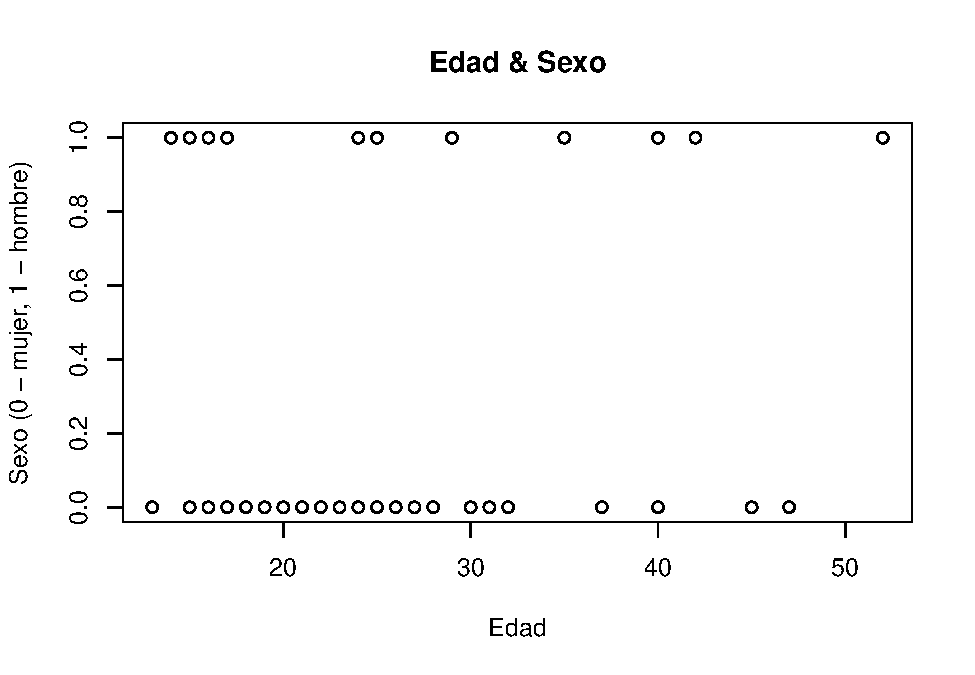
\includegraphics{codigo_files/figure-latex/grafico_edad_sexo-1.pdf}

Lo pasamos a PDF:

\begin{Shaded}
\begin{Highlighting}[]
\KeywordTok{pdf}\NormalTok{(}\StringTok{"Imágenes Obtenidas/GráficoEdad-Sexo.pdf"}\NormalTok{)}

\KeywordTok{plot}\NormalTok{(matriz.pacientes.datos[,}\DecValTok{1}\NormalTok{], matriz.pacientes.datos[,}\DecValTok{2}\NormalTok{], }\DataTypeTok{xlab=}\StringTok{"Edad"}\NormalTok{, }\DataTypeTok{ylab=}\StringTok{"Sexo (0 - mujer, 1 - hombre)"}\NormalTok{, }\DataTypeTok{main=}\StringTok{"Edad & Sexo"}\NormalTok{)}

\NormalTok{dev.off}
\end{Highlighting}
\end{Shaded}

\begin{verbatim}
## function (which = dev.cur()) 
## {
##     if (which == 1) 
##         stop("cannot shut down device 1 (the null device)")
##     .External(C_devoff, as.integer(which))
##     dev.cur()
## }
## <bytecode: 0x0000000015754360>
## <environment: namespace:grDevices>
\end{verbatim}

Otro plot para ver la correlación entre ser agresivo y ser impulsivo

\begin{Shaded}
\begin{Highlighting}[]
\NormalTok{rf <-}\StringTok{ }\KeywordTok{colorRampPalette}\NormalTok{(}\KeywordTok{rev}\NormalTok{(}\KeywordTok{brewer.pal}\NormalTok{(}\DecValTok{4}\NormalTok{,}\StringTok{'Spectral'}\NormalTok{)))}
\NormalTok{df <-}\StringTok{ }\KeywordTok{data.frame}\NormalTok{(matriz.pacientes.datos[, }\DecValTok{23}\NormalTok{], matriz.pacientes.datos[, }\DecValTok{24}\NormalTok{])}
\NormalTok{h <-}\StringTok{ }\KeywordTok{hexbin}\NormalTok{(df)}

\KeywordTok{plot}\NormalTok{(h, }\DataTypeTok{colramp=}\NormalTok{rf, }\DataTypeTok{xlab=}\StringTok{"Agresivo"}\NormalTok{, }\DataTypeTok{ylab=}\StringTok{"Impulsivo"}\NormalTok{, }\DataTypeTok{main=}\StringTok{"Agresivo Vs Impulsivo"}\NormalTok{)}
\end{Highlighting}
\end{Shaded}

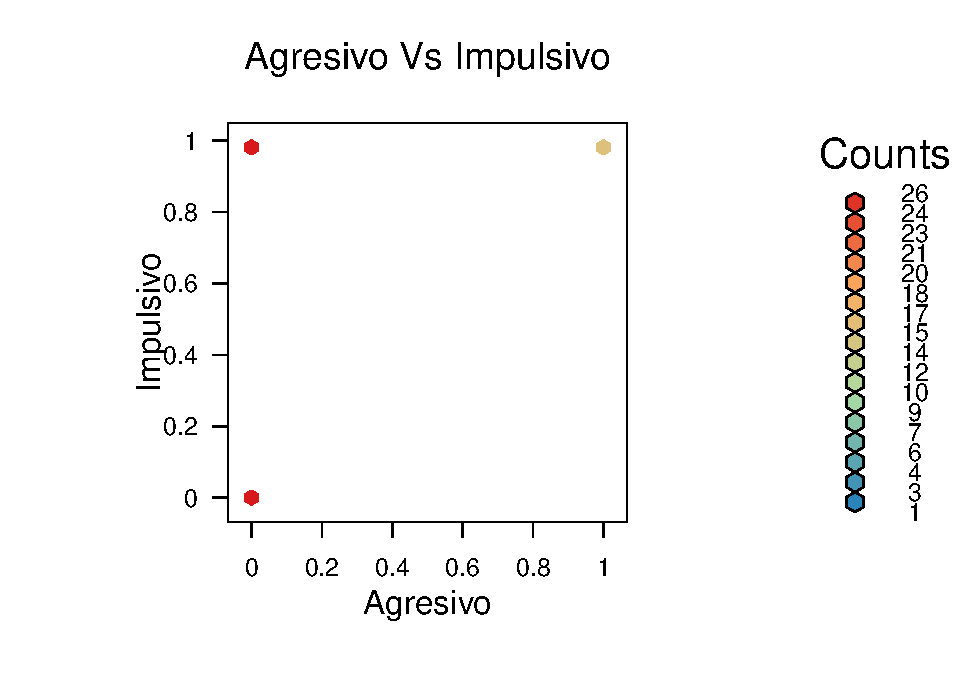
\includegraphics{codigo_files/figure-latex/grafico_agresivo_impulsivo-1.pdf}

Lo pasamos a PDF:

\begin{Shaded}
\begin{Highlighting}[]
\KeywordTok{pdf}\NormalTok{(}\StringTok{"Imágenes Obtenidas/GraficoAgresivoVsImpulsivo.pdf"}\NormalTok{)}

\KeywordTok{plot}\NormalTok{(h, }\DataTypeTok{colramp=}\NormalTok{rf, }\DataTypeTok{xlab=}\StringTok{"Agresivo"}\NormalTok{, }\DataTypeTok{ylab=}\StringTok{"Impulsivo"}\NormalTok{, }\DataTypeTok{main=}\StringTok{"Agresivo Vs Impulsivo"}\NormalTok{)}

\NormalTok{dev.off}
\end{Highlighting}
\end{Shaded}

\begin{verbatim}
## function (which = dev.cur()) 
## {
##     if (which == 1) 
##         stop("cannot shut down device 1 (the null device)")
##     .External(C_devoff, as.integer(which))
##     dev.cur()
## }
## <bytecode: 0x0000000015754360>
## <environment: namespace:grDevices>
\end{verbatim}

Otro plot similar para ver la relación de ser inhibido e impulsivo

\begin{Shaded}
\begin{Highlighting}[]
\NormalTok{df <-}\StringTok{ }\KeywordTok{data.frame}\NormalTok{(matriz.pacientes.datos[, }\DecValTok{21}\NormalTok{], matriz.pacientes.datos[, }\DecValTok{24}\NormalTok{])}
\NormalTok{h <-}\StringTok{ }\KeywordTok{hexbin}\NormalTok{(df)}

\KeywordTok{plot}\NormalTok{(h, }\DataTypeTok{colramp=}\NormalTok{rf, }\DataTypeTok{xlab=}\StringTok{"Inhibido"}\NormalTok{, }\DataTypeTok{ylab=}\StringTok{"Impulsivo"}\NormalTok{, }\DataTypeTok{main=}\StringTok{"Inhibido Vs Impulsivo"}\NormalTok{)}
\end{Highlighting}
\end{Shaded}

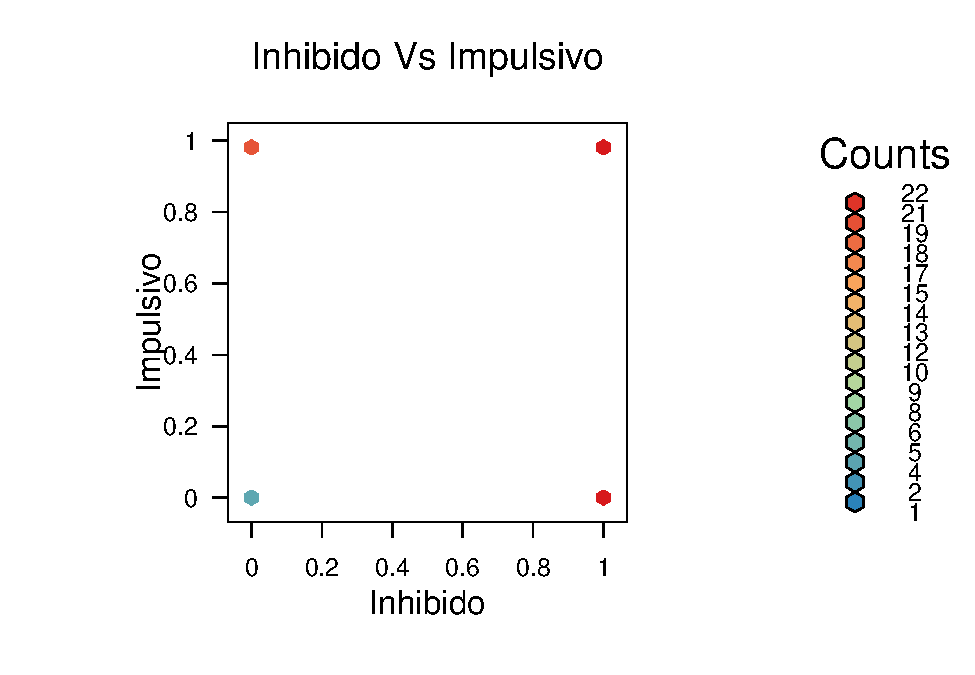
\includegraphics{codigo_files/figure-latex/grafico_inhibido_impulsivo-1.pdf}

Lo guardo en PDF:

\begin{Shaded}
\begin{Highlighting}[]
\KeywordTok{pdf}\NormalTok{(}\StringTok{"Imágenes Obtenidas/GraficoInhibidoVsImpulsivo.pdf"}\NormalTok{)}

\KeywordTok{plot}\NormalTok{(h, }\DataTypeTok{colramp=}\NormalTok{rf, }\DataTypeTok{xlab=}\StringTok{"Inhibido"}\NormalTok{, }\DataTypeTok{ylab=}\StringTok{"Impulsivo"}\NormalTok{, }\DataTypeTok{main=}\StringTok{"Inhibido Vs Impulsivo"}\NormalTok{)}

\NormalTok{dev.off}
\end{Highlighting}
\end{Shaded}

\begin{verbatim}
## function (which = dev.cur()) 
## {
##     if (which == 1) 
##         stop("cannot shut down device 1 (the null device)")
##     .External(C_devoff, as.integer(which))
##     dev.cur()
## }
## <bytecode: 0x0000000015754360>
## <environment: namespace:grDevices>
\end{verbatim}

Voy a ver la relación entre el razonamiento emocional (actuar según tus
sentimientos) y la impulsividad

\begin{Shaded}
\begin{Highlighting}[]
\NormalTok{df <-}\StringTok{ }\KeywordTok{data.frame}\NormalTok{(matriz.pacientes.datos[, }\DecValTok{20}\NormalTok{], matriz.pacientes.datos[, }\DecValTok{24}\NormalTok{])}
\NormalTok{h <-}\StringTok{ }\KeywordTok{hexbin}\NormalTok{(df)}

\KeywordTok{plot}\NormalTok{(h, }\DataTypeTok{colramp=}\NormalTok{rf, }\DataTypeTok{xlab=}\StringTok{"Razonamiento Emocional"}\NormalTok{, }\DataTypeTok{ylab=}\StringTok{"Impulsivo"}\NormalTok{, }\DataTypeTok{main=}\StringTok{"Razonamiento Emocional Vs Impulsivo"}\NormalTok{)}
\end{Highlighting}
\end{Shaded}

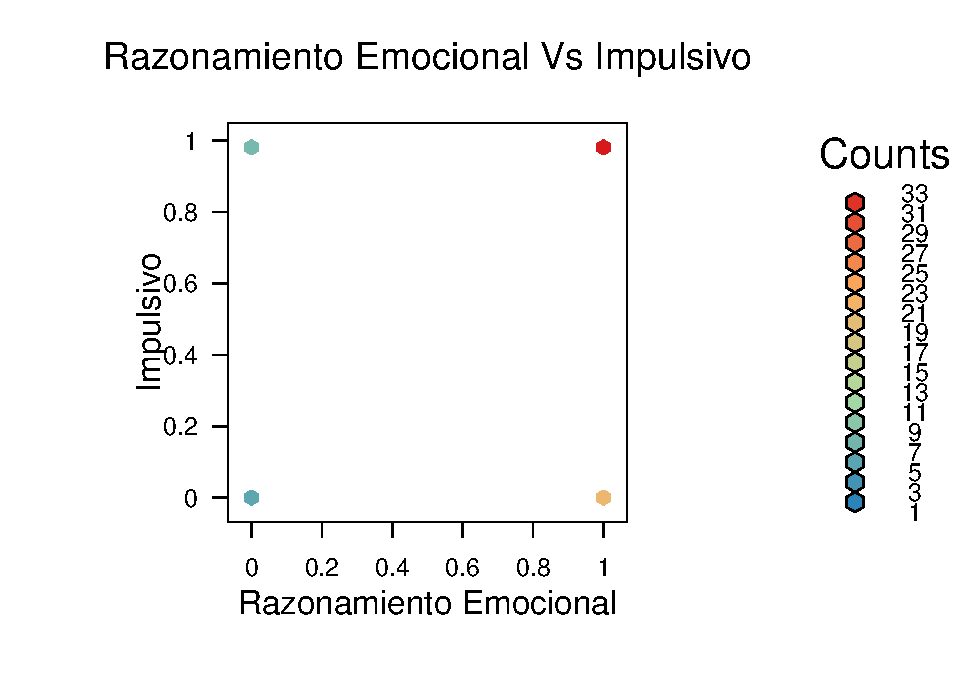
\includegraphics{codigo_files/figure-latex/grafico_razEm_Impulsivo-1.pdf}

Lo guardo en PDF:

\begin{Shaded}
\begin{Highlighting}[]
\KeywordTok{pdf}\NormalTok{(}\StringTok{"Imágenes Obtenidas/GraficoRazonamientoEmocionalVsImpulsivo.pdf"}\NormalTok{)}

\KeywordTok{plot}\NormalTok{(h, }\DataTypeTok{colramp=}\NormalTok{rf, }\DataTypeTok{xlab=}\StringTok{"Razonamiento Emocional"}\NormalTok{, }\DataTypeTok{ylab=}\StringTok{"Impulsivo"}\NormalTok{, }\DataTypeTok{main=}\StringTok{"Razonamiento Emocional Vs Impulsivo"}\NormalTok{)}

\NormalTok{dev.off}
\end{Highlighting}
\end{Shaded}

\begin{verbatim}
## function (which = dev.cur()) 
## {
##     if (which == 1) 
##         stop("cannot shut down device 1 (the null device)")
##     .External(C_devoff, as.integer(which))
##     dev.cur()
## }
## <bytecode: 0x0000000015754360>
## <environment: namespace:grDevices>
\end{verbatim}

Ahora quiero sacar una relación entre ser agresivo y ver el grupo en el
que están

\begin{Shaded}
\begin{Highlighting}[]
\NormalTok{rf <-}\StringTok{ }\KeywordTok{colorRampPalette}\NormalTok{(}\KeywordTok{rev}\NormalTok{(}\KeywordTok{brewer.pal}\NormalTok{(}\DecValTok{4}\NormalTok{,}\StringTok{'Spectral'}\NormalTok{)))}
\NormalTok{df <-}\StringTok{ }\KeywordTok{data.frame}\NormalTok{(matriz.pacientes.datos[, }\DecValTok{23}\NormalTok{], matriz.pacientes.etiquetas[, }\DecValTok{25}\NormalTok{])}
\NormalTok{h <-}\StringTok{ }\KeywordTok{hexbin}\NormalTok{(df)}

\KeywordTok{plot}\NormalTok{(h, }\DataTypeTok{colramp=}\NormalTok{rf, }\DataTypeTok{xlab=}\StringTok{"Agresivo"}\NormalTok{, }\DataTypeTok{ylab=}\StringTok{"Grupo"}\NormalTok{, }\DataTypeTok{main=}\StringTok{"Agresivo Y Grupo Real"}\NormalTok{)}
\end{Highlighting}
\end{Shaded}

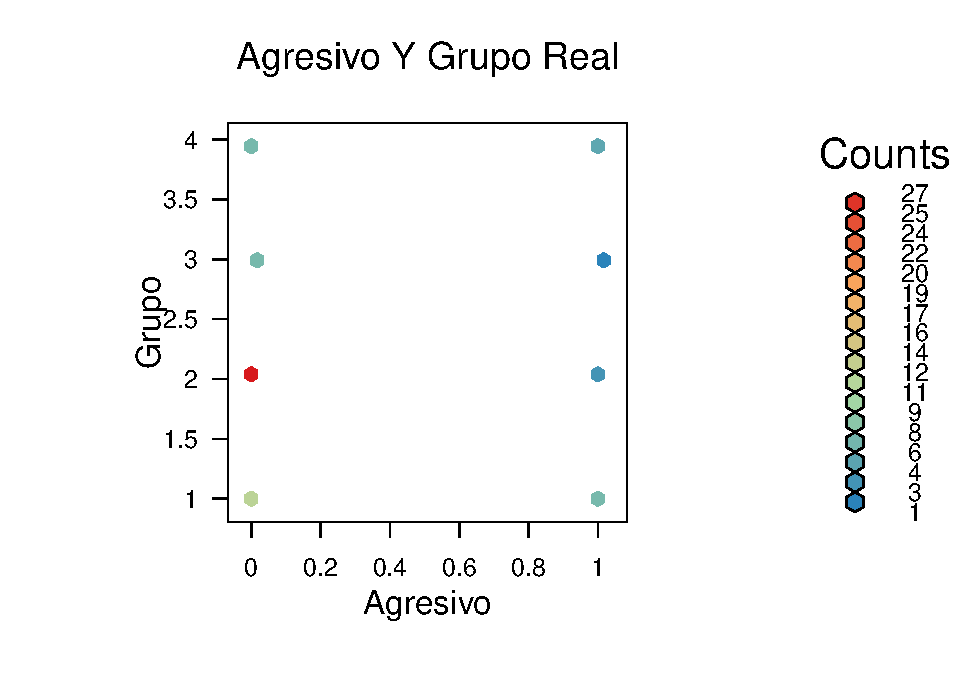
\includegraphics{codigo_files/figure-latex/grafico_agresivo_grupo-1.pdf}

Lo guardo en PDF:

\begin{Shaded}
\begin{Highlighting}[]
\KeywordTok{pdf}\NormalTok{(}\StringTok{"Imágenes Obtenidas/GraficoAgresivoVsGrupo.pdf"}\NormalTok{)}

\KeywordTok{plot}\NormalTok{(h, }\DataTypeTok{colramp=}\NormalTok{rf, }\DataTypeTok{xlab=}\StringTok{"Agresivo"}\NormalTok{, }\DataTypeTok{ylab=}\StringTok{"Grupo"}\NormalTok{, }\DataTypeTok{main=}\StringTok{"Agresivo Y Grupo Real"}\NormalTok{)}

\NormalTok{dev.off}
\end{Highlighting}
\end{Shaded}

\begin{verbatim}
## function (which = dev.cur()) 
## {
##     if (which == 1) 
##         stop("cannot shut down device 1 (the null device)")
##     .External(C_devoff, as.integer(which))
##     dev.cur()
## }
## <bytecode: 0x0000000015754360>
## <environment: namespace:grDevices>
\end{verbatim}

Voy a hacer lo mismo con la impulsividad

\begin{Shaded}
\begin{Highlighting}[]
\NormalTok{rf <-}\StringTok{ }\KeywordTok{colorRampPalette}\NormalTok{(}\KeywordTok{rev}\NormalTok{(}\KeywordTok{brewer.pal}\NormalTok{(}\DecValTok{4}\NormalTok{,}\StringTok{'Spectral'}\NormalTok{)))}
\NormalTok{df <-}\StringTok{ }\KeywordTok{data.frame}\NormalTok{(matriz.pacientes.datos[, }\DecValTok{24}\NormalTok{], matriz.pacientes.etiquetas[, }\DecValTok{25}\NormalTok{])}
\NormalTok{h <-}\StringTok{ }\KeywordTok{hexbin}\NormalTok{(df)}

\KeywordTok{plot}\NormalTok{(h, }\DataTypeTok{colramp=}\NormalTok{rf, }\DataTypeTok{xlab=}\StringTok{"Impulsivo"}\NormalTok{, }\DataTypeTok{ylab=}\StringTok{"Grupo"}\NormalTok{, }\DataTypeTok{main=}\StringTok{"Impulsivo y Grupo Real"}\NormalTok{)}
\end{Highlighting}
\end{Shaded}

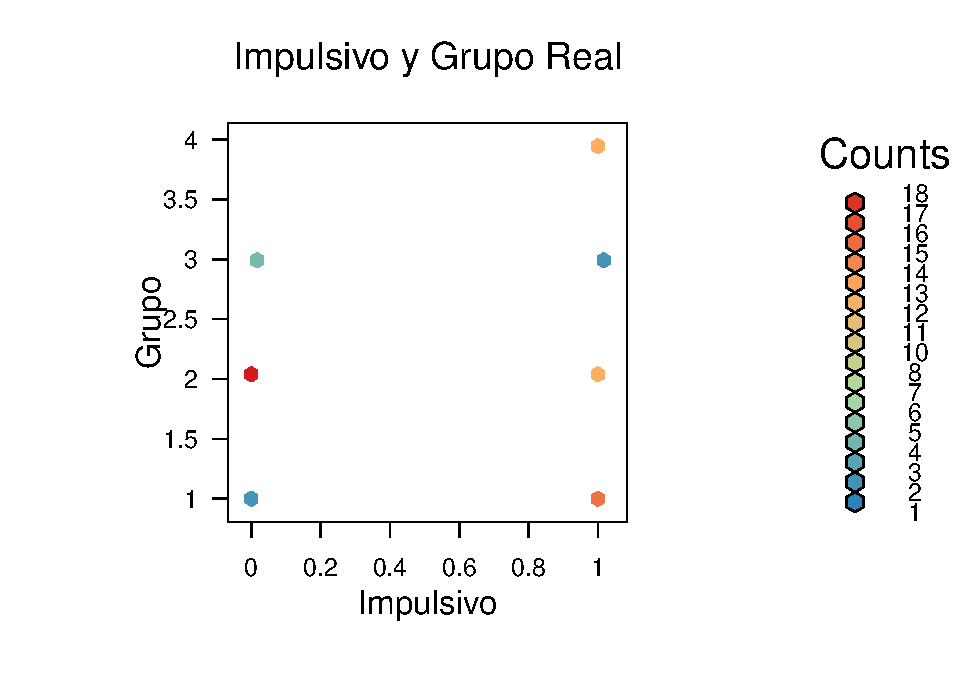
\includegraphics{codigo_files/figure-latex/grafico_impulsivo_grupo-1.pdf}

Lo guardo en PDF:

\begin{Shaded}
\begin{Highlighting}[]
\KeywordTok{pdf}\NormalTok{(}\StringTok{"Imágenes Obtenidas/GraficoImpulsivoVsGrupo.pdf"}\NormalTok{)}

\KeywordTok{plot}\NormalTok{(h, }\DataTypeTok{colramp=}\NormalTok{rf, }\DataTypeTok{xlab=}\StringTok{"Impulsivo"}\NormalTok{, }\DataTypeTok{ylab=}\StringTok{"Grupo"}\NormalTok{, }\DataTypeTok{main=}\StringTok{"Impulsivo y Grupo Real"}\NormalTok{)}

\NormalTok{dev.off}
\end{Highlighting}
\end{Shaded}

\begin{verbatim}
## function (which = dev.cur()) 
## {
##     if (which == 1) 
##         stop("cannot shut down device 1 (the null device)")
##     .External(C_devoff, as.integer(which))
##     dev.cur()
## }
## <bytecode: 0x0000000015754360>
## <environment: namespace:grDevices>
\end{verbatim}

De estas gráficas estamos obteniendo información realmente interesante
antes de la predicción de los datos. He preferido hacer gráficas en 2D
porque las gráficas en 3D son mucho más difíciles de interpretar que
estas bonitas gráficas en 2D

Vamos a ver la correlación que tienen mis variables

\begin{Shaded}
\begin{Highlighting}[]
\NormalTok{res <-}\StringTok{ }\KeywordTok{cor}\NormalTok{(matriz.pacientes.datos[, }\DecValTok{1}\OperatorTok{:}\DecValTok{24}\NormalTok{], }\DataTypeTok{method =} \StringTok{"spearman"}\NormalTok{) }\CommentTok{# Por mi tipo de datos, hacemos la correlación por spearman}
\KeywordTok{options}\NormalTok{(}\DataTypeTok{width =} \DecValTok{100}\NormalTok{)}
\NormalTok{res.round <-}\StringTok{ }\KeywordTok{round}\NormalTok{(res, }\DecValTok{2}\NormalTok{)}
\end{Highlighting}
\end{Shaded}

Como saca una tabla enorme, lo que voy a hacer es usar una librería que
me da una función para sacar de una forma bonita las correlaciones entre
las variables.

\begin{Shaded}
\begin{Highlighting}[]
\KeywordTok{corrplot}\NormalTok{(res.round, }\DataTypeTok{method=}\StringTok{"circle"}\NormalTok{)}
\end{Highlighting}
\end{Shaded}

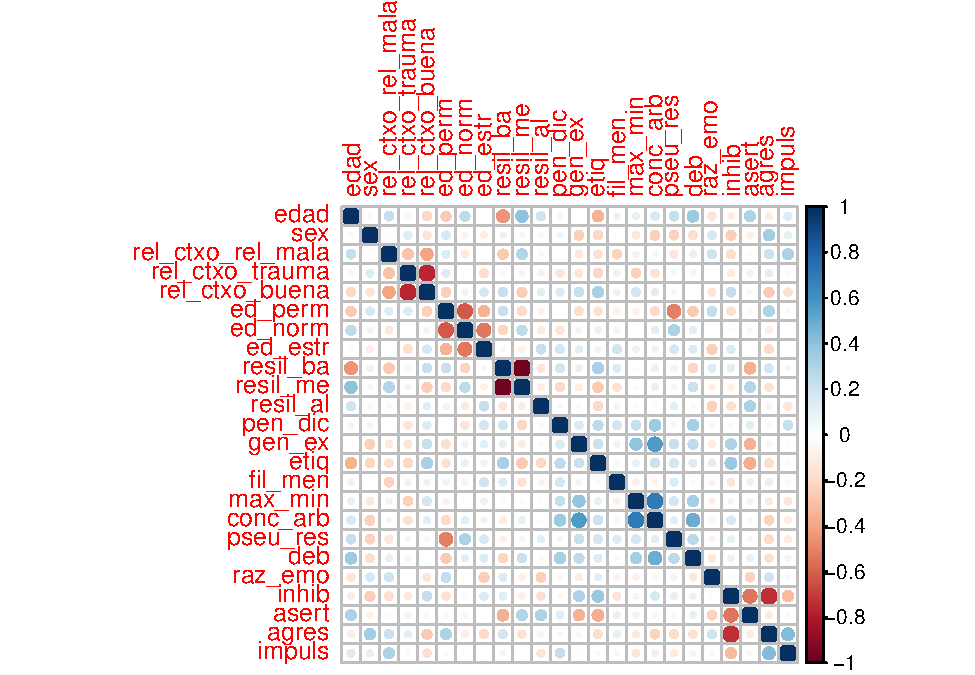
\includegraphics{codigo_files/figure-latex/grafico_correlaciones_variables-1.pdf}

Guardamos la matriz de correlación en PDF para tener mejor
visualización:

\begin{Shaded}
\begin{Highlighting}[]
\KeywordTok{pdf}\NormalTok{(}\StringTok{"Imágenes Obtenidas/Corrplot.pdf"}\NormalTok{)}

\KeywordTok{corrplot}\NormalTok{(res.round, }\DataTypeTok{method=}\StringTok{"circle"}\NormalTok{)}

\NormalTok{dev.off}
\end{Highlighting}
\end{Shaded}

\begin{verbatim}
## function (which = dev.cur()) 
## {
##     if (which == 1) 
##         stop("cannot shut down device 1 (the null device)")
##     .External(C_devoff, as.integer(which))
##     dev.cur()
## }
## <bytecode: 0x0000000015754360>
## <environment: namespace:grDevices>
\end{verbatim}

Como podemos ver, por ejemplo, resiliencia baja y media tienen una
correlación de -1, ya que si hay una no hay la otra y viceversa. Esto
pasa igual con las relaciones entre contexto, ya que buena - trauma,
trauma - mala, mala - buena tienen que ser inversas.

Ahora voy a sacar un PCA para ver la importancia de las variables:

Para los cálculos, uso la matriz con el centrado y escalado ya hechos

\begin{Shaded}
\begin{Highlighting}[]
\NormalTok{resultado.pca <-}\StringTok{ }\KeywordTok{PCA}\NormalTok{(matriz.pacientes.datos.centscal, }\DataTypeTok{graph =} \OtherTok{FALSE}\NormalTok{)}

\CommentTok{#Con la siguiente línea podemos ver que podemos hacer con esto calculado}
\KeywordTok{print}\NormalTok{(resultado.pca)}
\end{Highlighting}
\end{Shaded}

\begin{verbatim}
## **Results for the Principal Component Analysis (PCA)**
## The analysis was performed on 67 individuals, described by 24 variables
## *The results are available in the following objects:
## 
##    name               description                          
## 1  "$eig"             "eigenvalues"                        
## 2  "$var"             "results for the variables"          
## 3  "$var$coord"       "coord. for the variables"           
## 4  "$var$cor"         "correlations variables - dimensions"
## 5  "$var$cos2"        "cos2 for the variables"             
## 6  "$var$contrib"     "contributions of the variables"     
## 7  "$ind"             "results for the individuals"        
## 8  "$ind$coord"       "coord. for the individuals"         
## 9  "$ind$cos2"        "cos2 for the individuals"           
## 10 "$ind$contrib"     "contributions of the individuals"   
## 11 "$call"            "summary statistics"                 
## 12 "$call$centre"     "mean of the variables"              
## 13 "$call$ecart.type" "standard error of the variables"    
## 14 "$call$row.w"      "weights for the individuals"        
## 15 "$call$col.w"      "weights for the variables"
\end{verbatim}

Nos interesa ver los eigenvalues, que son los que presentarán la
cantidad de varianza que aportan las variables:

\begin{Shaded}
\begin{Highlighting}[]
\NormalTok{eigenvalues.PCA <-}\StringTok{ }\NormalTok{resultado.pca}\OperatorTok{$}\NormalTok{eig}
\NormalTok{eigenvalues.PCA}
\end{Highlighting}
\end{Shaded}

\begin{verbatim}
##           eigenvalue percentage of variance cumulative percentage of variance
## comp 1  3.896946e+00           1.623727e+01                          16.23727
## comp 2  3.348839e+00           1.395349e+01                          30.19077
## comp 3  2.189584e+00           9.123265e+00                          39.31403
## comp 4  2.044520e+00           8.518834e+00                          47.83287
## comp 5  1.737900e+00           7.241252e+00                          55.07412
## comp 6  1.521215e+00           6.338397e+00                          61.41252
## comp 7  1.374042e+00           5.725176e+00                          67.13769
## comp 8  1.079722e+00           4.498843e+00                          71.63653
## comp 9  9.591848e-01           3.996603e+00                          75.63314
## comp 10 9.311536e-01           3.879807e+00                          79.51294
## comp 11 8.644377e-01           3.601824e+00                          83.11477
## comp 12 8.099267e-01           3.374695e+00                          86.48946
## comp 13 6.658121e-01           2.774217e+00                          89.26368
## comp 14 5.935233e-01           2.473014e+00                          91.73669
## comp 15 4.698651e-01           1.957771e+00                          93.69447
## comp 16 4.632196e-01           1.930082e+00                          95.62455
## comp 17 3.922638e-01           1.634433e+00                          97.25898
## comp 18 2.445767e-01           1.019069e+00                          98.27805
## comp 19 2.251255e-01           9.380229e-01                          99.21607
## comp 20 1.497768e-01           6.240699e-01                          99.84014
## comp 21 3.836592e-02           1.598580e-01                         100.00000
## comp 22 9.366318e-32           3.902633e-31                         100.00000
## comp 23 8.328156e-32           3.470065e-31                         100.00000
## comp 24 3.135473e-32           1.306447e-31                         100.00000
\end{verbatim}

Como se puede comprobar, de las 24 variables (componentes) que tenemos,
la mitad de la varianza la conseguimos con aproximadamente 5 variables.
También se puede ver que a parti de las 17 variables prácticamente no
hay un aumento de la varianza. En el caso de un problema grande, sería
interesante la eliminación de algunas de las variables, para dejar un
dataset más pequeño con el que poder trabajar. En nuestro caso, nuestro
problema es pequeño, y además las variables están escogidas a mano, por
lo que no haré una reducción del dataset.

Ahora, para completar este apartado de PCA, lo que voy a hacer es sacar
la gráfica de la varianza acumulada con los valores anteriores:

\begin{Shaded}
\begin{Highlighting}[]
\NormalTok{plotPCA <-}\StringTok{ }\KeywordTok{fviz_screeplot}\NormalTok{(resultado.pca, }\DataTypeTok{ncp=}\DecValTok{24}\NormalTok{)}
\KeywordTok{plot}\NormalTok{(plotPCA)}
\end{Highlighting}
\end{Shaded}

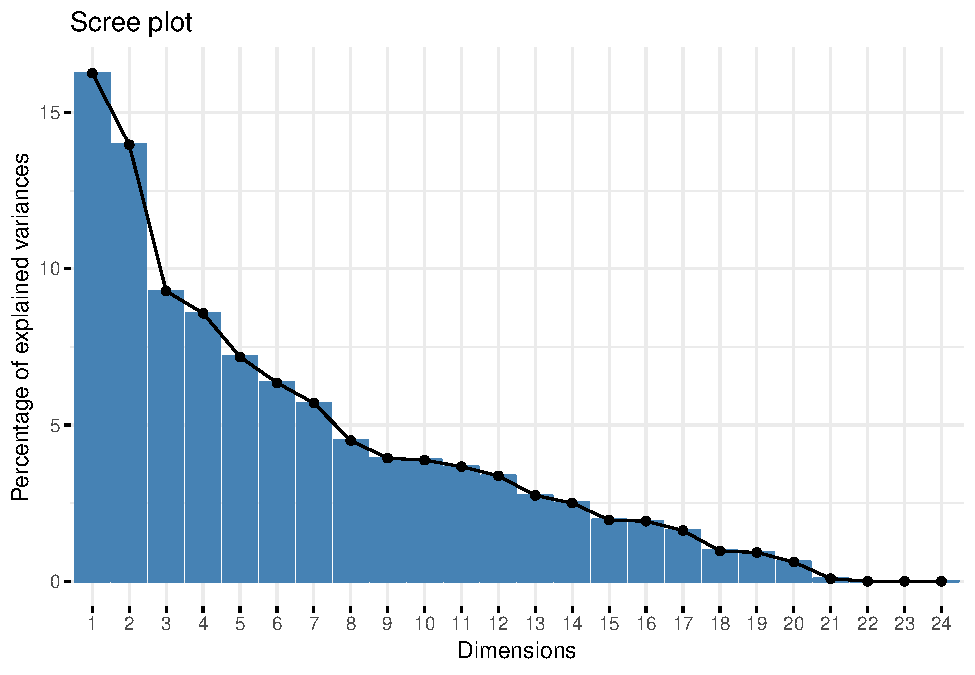
\includegraphics{codigo_files/figure-latex/PCA_eigenvalues_graph-1.pdf}

Obtengo este gráfico en PDF para tener una mejor visualización:

\begin{Shaded}
\begin{Highlighting}[]
\KeywordTok{pdf}\NormalTok{(}\StringTok{"Imágenes Obtenidas/GraficoEigenvalues.pdf"}\NormalTok{)}

\KeywordTok{plot}\NormalTok{(plotPCA)}

\NormalTok{dev.off}
\end{Highlighting}
\end{Shaded}

\begin{verbatim}
## function (which = dev.cur()) 
## {
##     if (which == 1) 
##         stop("cannot shut down device 1 (the null device)")
##     .External(C_devoff, as.integer(which))
##     dev.cur()
## }
## <bytecode: 0x0000000015754360>
## <environment: namespace:grDevices>
\end{verbatim}

Ahora voy a sacar un ``Factor Map'' de las variables. Esto lo puedo
hacer gracias a las coordenadas que me da una de las variables tras
hacer el PCA. Así, voy primero a ver la tabla y luego voy a sacar el
mapa:

\begin{Shaded}
\begin{Highlighting}[]
\NormalTok{resultado.pca}\OperatorTok{$}\NormalTok{var}\OperatorTok{$}\NormalTok{coord}
\end{Highlighting}
\end{Shaded}

\begin{verbatim}
##                          Dim.1       Dim.2       Dim.3        Dim.4       Dim.5
## edad               0.007991017  0.66451493  0.19586260  0.007841951  0.02805228
## sex               -0.447913174 -0.11533971  0.10245651  0.057192465  0.11492883
## rel_ctxo_rel_mala -0.234645431  0.31242667  0.16869825  0.565844840 -0.35019764
## rel_ctxo_trauma   -0.417381244  0.11742230 -0.21001522 -0.136376092  0.34458474
## rel_ctxo_buena     0.560339731 -0.32571613  0.08634947 -0.255162421 -0.09161091
## ed_perm           -0.553915390 -0.34063941  0.23874352  0.241008740 -0.33289199
## ed_norm            0.195717913  0.33691768 -0.54551596  0.069259334  0.57202966
## ed_estr            0.364218109 -0.03574847  0.39611368 -0.343671891 -0.32610946
## resil_ba           0.051112365 -0.85796492  0.20216746 -0.039061871  0.21241196
## resil_me          -0.074743641  0.80191325 -0.29969255  0.153867444 -0.18199709
## resil_al           0.095173049  0.24393919  0.39293737 -0.466258490 -0.12766293
## pen_dic            0.311964031 -0.08886036  0.58511514  0.186141485  0.18431008
## gen_ex             0.595148670 -0.10912103  0.08286185  0.282531851  0.16255400
## etiq               0.499365039 -0.45912251 -0.17281954  0.173075672  0.14741419
## fil_men            0.059354773 -0.07552104  0.31916448 -0.355626217  0.39559535
## max_min            0.524773891  0.12325520  0.31096225  0.378637566 -0.01643986
## conc_arb           0.645068936  0.21765964  0.22093906  0.466271365  0.04542650
## pseu_res           0.443972323  0.22314014 -0.11950533 -0.176808668  0.43526671
## deb                0.484524206  0.38834362  0.18502988  0.268386661  0.11400205
## raz_emo           -0.251049993 -0.27394959 -0.20413968  0.433531845  0.02071493
## inhib              0.563528317 -0.27772651 -0.48974596  0.018053816 -0.35529325
## asert             -0.126327074  0.57800397  0.34437650 -0.343315766  0.04021108
## agres             -0.591302668 -0.14500954  0.29219301  0.239210208  0.43081535
## impuls            -0.289816690  0.01403726  0.32193103  0.339678159  0.27914883
\end{verbatim}

Como se puede ver, me está poniendo mis 24 variables en 5 dimensiones,
con unas coordenadas concretas. Ahora, lo que voy a hacer, es
representarlo. Con esta representación podré sacar algunas conclusiones:

\begin{Shaded}
\begin{Highlighting}[]
\KeywordTok{fviz_pca_var}\NormalTok{(resultado.pca)}
\end{Highlighting}
\end{Shaded}

\includegraphics{codigo_files/figure-latex/PCA_Coordinates_Graph-1.pdf}

Exporto a PDF este gráfico de coordenadas:

\begin{Shaded}
\begin{Highlighting}[]
\KeywordTok{pdf}\NormalTok{(}\StringTok{"Imágenes Obtenidas/GraficoVectoresVariablesPCA.pdf"}\NormalTok{)}

\KeywordTok{fviz_pca_var}\NormalTok{(resultado.pca)}

\NormalTok{dev.off}
\end{Highlighting}
\end{Shaded}

\begin{verbatim}
## function (which = dev.cur()) 
## {
##     if (which == 1) 
##         stop("cannot shut down device 1 (the null device)")
##     .External(C_devoff, as.integer(which))
##     dev.cur()
## }
## <bytecode: 0x0000000015754360>
## <environment: namespace:grDevices>
\end{verbatim}

Con esto puedo sacar conclusiones al igual que con el gran gráfico de
correlaciones de variables, solo que esta representación está
intencionada para más de 2 dimensiones.

Puedo ver algunas de las conclusiones fáciles que saqué anteriormente,
como que resiliencia media es contraria a baja, o que la relación con el
contexto de trauma y mala son contrarias a buena.

Otras relaciones también puedo ver, como que los deberías y el
razonamiento emocional parecen ser ciertamente contrarios, o que el
filtro mental no depende de prácticamente nada ya que está en todo el
centro.

También es importante ver como, mediante dos componentes principales
(dos dimensiones), solo estoy explicando un del 30,2\% del total, lo que
es muy poco. Por unirlo con los gráficos anteriores, estas dos
componentes que se han elegido como x e y son las dos variables que más
varianza (y por lo tanto, explicación) tenían en el gráfico de barras
anterior.

Ahora mi siguiente paso es sacar un gráfico de los individuos, para ver
donde están colocados en este sistema:

\begin{Shaded}
\begin{Highlighting}[]
\KeywordTok{head}\NormalTok{(resultado.pca}\OperatorTok{$}\NormalTok{ind}\OperatorTok{$}\NormalTok{coord) }\CommentTok{# Solo saco los primeros para no ocupar demasiado espacio}
\end{Highlighting}
\end{Shaded}

\begin{verbatim}
##        Dim.1     Dim.2      Dim.3      Dim.4      Dim.5
## 1 -2.3243690  2.147815 -1.1849618  2.4481512 -0.7586328
## 2  2.4647257 -1.262473  0.2217190 -1.1784100 -1.4473760
## 3  0.6387125 -2.080331 -0.1818521  0.7676582 -2.0265412
## 4 -1.9384395 -1.832160  1.4628618  1.1820858  1.1852182
## 5  2.0986406  0.262897 -0.2150152 -0.7686587 -1.2663434
## 6  1.1578332 -1.323444 -0.8453683  0.9774806 -0.1661987
\end{verbatim}

Ahora, tras ver que todos mis individuos tienen unas ciertas
coordenadas, vamos a representarlos gráficamente:

\begin{Shaded}
\begin{Highlighting}[]
\KeywordTok{fviz_pca_ind}\NormalTok{(resultado.pca)}
\end{Highlighting}
\end{Shaded}

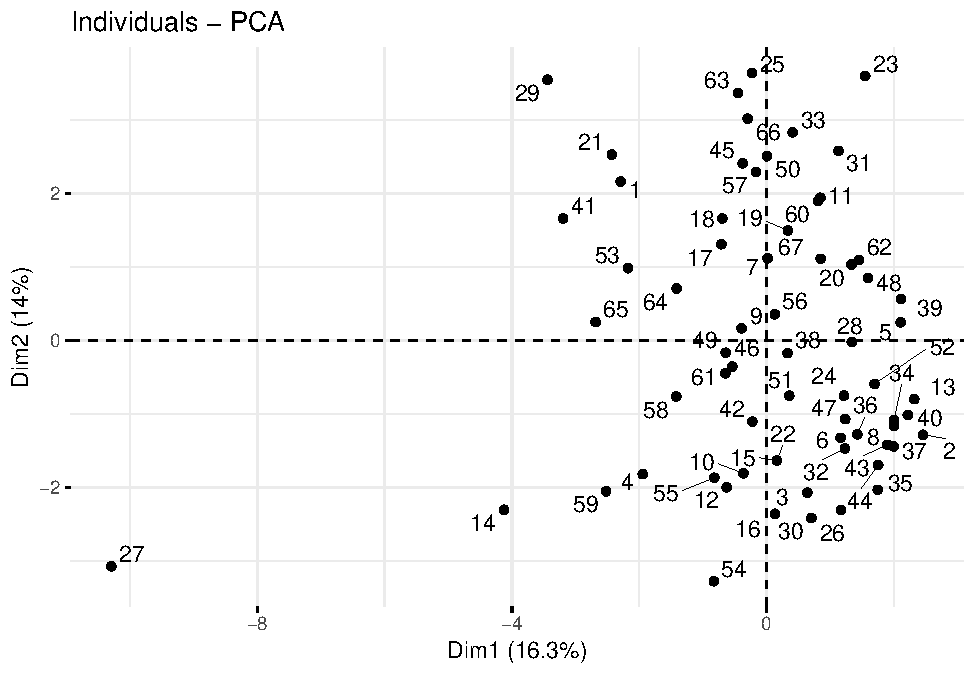
\includegraphics{codigo_files/figure-latex/plot_coordendas_individuos-1.pdf}

Exporto a PDF las coordenadas de los individuos:

\begin{Shaded}
\begin{Highlighting}[]
\KeywordTok{pdf}\NormalTok{(}\StringTok{"Imágenes Obtenidas/GraficoIndividuosPCA.pdf"}\NormalTok{)}

\KeywordTok{fviz_pca_ind}\NormalTok{(resultado.pca)}

\NormalTok{dev.off}
\end{Highlighting}
\end{Shaded}

\begin{verbatim}
## function (which = dev.cur()) 
## {
##     if (which == 1) 
##         stop("cannot shut down device 1 (the null device)")
##     .External(C_devoff, as.integer(which))
##     dev.cur()
## }
## <bytecode: 0x0000000015754360>
## <environment: namespace:grDevices>
\end{verbatim}

Se puede ver que la mayoría de los pacientes están en torno al centro,
mientras que tenemos un outlayer, que es el número 27.

\begin{center}\rule{0.5\linewidth}{\linethickness}\end{center}

\section{Modelos de Inteligencia Artificial
supervisados}\label{modelos-de-inteligencia-artificial-supervisados}

Ahora lo que hago es coger un conjunto muy grande de los datos para
hacer el entrenamiento

\begin{Shaded}
\begin{Highlighting}[]
\NormalTok{conjuntoEntrenamiento <-}\StringTok{ }\KeywordTok{sample}\NormalTok{(}\DecValTok{1}\OperatorTok{:}\DecValTok{67}\NormalTok{, }\DecValTok{55}\NormalTok{)}
\end{Highlighting}
\end{Shaded}

1 NEURONA

Lo que voy a hacer ahora es entrenar la red neuronal con diferente
cantidad de neuronas,y voy a ir comparando el resultado\ldots{}

SIN SOFTMAX

\begin{Shaded}
\begin{Highlighting}[]
\KeywordTok{set.seed}\NormalTok{(}\DecValTok{1}\NormalTok{)}

\NormalTok{dataframe.resultados.1neu <-}\StringTok{ }\KeywordTok{data.frame}\NormalTok{(}\DataTypeTok{Ent_1Neu =} \KeywordTok{numeric}\NormalTok{(),}
                                        \DataTypeTok{Test_1Neu =} \KeywordTok{numeric}\NormalTok{())}

\ControlFlowTok{for}\NormalTok{(i }\ControlFlowTok{in} \DecValTok{1}\OperatorTok{:}\DecValTok{20}\NormalTok{)}
\NormalTok{\{}
\NormalTok{  pacientes.1neu <-}\StringTok{ }\KeywordTok{nnet}\NormalTok{( matriz.pacientes.datos.centscal[conjuntoEntrenamiento, }\DecValTok{1}\OperatorTok{:}\DecValTok{24}\NormalTok{], }\KeywordTok{class.ind}\NormalTok{( matriz.pacientes.etiquetas[conjuntoEntrenamiento, }\DecValTok{25}\NormalTok{] ) , }\DataTypeTok{size=}\DecValTok{1}\NormalTok{)}

  \CommentTok{#Una vez que lo tengo entrenado, lo que voy a hacer es calcular el error tanto en el entrenamiento como en el test de cada uno}
  
\NormalTok{  pacientes.prediccion.1neu <-}\StringTok{ }\KeywordTok{predict}\NormalTok{( pacientes.1neu, matriz.pacientes.datos.centscal[conjuntoEntrenamiento, }\DecValTok{1}\OperatorTok{:}\DecValTok{24}\NormalTok{], }\DataTypeTok{type=}\StringTok{"raw"}\NormalTok{ )}
  \KeywordTok{head}\NormalTok{(pacientes.prediccion.1neu) }\CommentTok{# Vemos las probabilidades de pertenencia de cada valor}
  
  \CommentTok{# Ahora que los tengo todos entrenados, Determinamos cual es la máxima, es decir, la clase a la que hay que asignar los objetos}
  
\NormalTok{  pacientes.prediccion.1neu.class <-}\StringTok{ }\KeywordTok{apply}\NormalTok{( pacientes.prediccion.1neu, }\DataTypeTok{MARGIN=}\DecValTok{1}\NormalTok{, }\DataTypeTok{FUN=}\StringTok{'which.is.max'}\NormalTok{)}
\NormalTok{  pacientes.prediccion.1neu.class}
  
  \CommentTok{# Lo visualizo en forma de tabla para ir viendo el error}
  
  \KeywordTok{table}\NormalTok{( pacientes.prediccion.1neu.class, matriz.pacientes.etiquetas[conjuntoEntrenamiento, }\DecValTok{25}\NormalTok{] )  }\CommentTok{# Lo vemos en forma de tabla.}
  
  \CommentTok{#Calculo el acierto}
  
\NormalTok{  acierto.ent.teorico.1neu <-}\StringTok{ }\KeywordTok{sum}\NormalTok{( }\KeywordTok{diag}\NormalTok{( }\KeywordTok{table}\NormalTok{( pacientes.prediccion.1neu.class, matriz.pacientes.etiquetas[conjuntoEntrenamiento, }\DecValTok{25}\NormalTok{] ) ) )}\OperatorTok{/}\DecValTok{55} \CommentTok{# Esta cuenta nos da el índice de acierto}
  
  \CommentTok{#TEST}
  
\NormalTok{  pacientes.prediccion.test.1neu <-}\StringTok{ }\KeywordTok{predict}\NormalTok{( pacientes.1neu, matriz.pacientes.datos.centscal[}\OperatorTok{-}\NormalTok{conjuntoEntrenamiento, }\DecValTok{1}\OperatorTok{:}\DecValTok{24}\NormalTok{], }\DataTypeTok{type=}\StringTok{"raw"}\NormalTok{ )}
\NormalTok{  pacientes.prediccion.test.1neu}
  
\NormalTok{  pacientes.prediccion.test.1neu.class <-}\StringTok{ }\KeywordTok{apply}\NormalTok{( pacientes.prediccion.test.1neu, }\DataTypeTok{MARGIN=}\DecValTok{1}\NormalTok{, }\DataTypeTok{FUN=}\StringTok{'which.is.max'}\NormalTok{)}
\NormalTok{  pacientes.prediccion.test.1neu.class}
  
  \KeywordTok{table}\NormalTok{( pacientes.prediccion.test.1neu.class , matriz.pacientes.etiquetas[}\OperatorTok{-}\NormalTok{conjuntoEntrenamiento, }\DecValTok{25}\NormalTok{] )}
\NormalTok{  acierto.test.teorico.1neu <-}\StringTok{ }\KeywordTok{sum}\NormalTok{( }\KeywordTok{diag}\NormalTok{( }\KeywordTok{table}\NormalTok{( pacientes.prediccion.test.1neu.class, matriz.pacientes.etiquetas[}\OperatorTok{-}\NormalTok{conjuntoEntrenamiento, }\DecValTok{25}\NormalTok{] ) ) )}\OperatorTok{/}\DecValTok{12}
  
\NormalTok{  dataframe.pasada <-}\StringTok{ }\KeywordTok{data.frame}\NormalTok{(}\DataTypeTok{Ent_1Neu =}\NormalTok{ acierto.ent.teorico.1neu,}
                                 \DataTypeTok{Test_1Neu =}\NormalTok{ acierto.test.teorico.1neu)}
  
\NormalTok{  dataframe.resultados.1neu <-}\StringTok{ }\KeywordTok{rbind}\NormalTok{(dataframe.resultados.1neu, dataframe.pasada)}

\NormalTok{\}}
\end{Highlighting}
\end{Shaded}

Lo voy a entrenar también con el SOFTMAX = true. Esto optimiza la
verosimilitud, no el error cuadrático medio\ldots{}
\#\#\#\#\#\#\#\#\#\#\#\#\#\#\#\#\#\#\#\#\#\# CON SOFTMAX
\#\#\#\#\#\#\#\#\#\#\#\#\#\#\#\#\#\#\#\#\#\#\#\#\#\#\#\#\#\#

\begin{Shaded}
\begin{Highlighting}[]
\KeywordTok{set.seed}\NormalTok{(}\DecValTok{1}\NormalTok{)}

\NormalTok{dataframe.resultados.1neu.soft <-}\StringTok{ }\KeywordTok{data.frame}\NormalTok{(}\DataTypeTok{Ent_1Neu_soft =} \KeywordTok{numeric}\NormalTok{(),}
                                             \DataTypeTok{Test_1Neu_soft =} \KeywordTok{numeric}\NormalTok{())}

\ControlFlowTok{for}\NormalTok{(i }\ControlFlowTok{in} \DecValTok{1}\OperatorTok{:}\DecValTok{20}\NormalTok{)}
\NormalTok{\{}
\NormalTok{  pacientes.1neu.softmax <-}\StringTok{ }\KeywordTok{nnet}\NormalTok{( matriz.pacientes.datos.centscal[conjuntoEntrenamiento, }\DecValTok{1}\OperatorTok{:}\DecValTok{24}\NormalTok{], }\KeywordTok{class.ind}\NormalTok{( matriz.pacientes.etiquetas[conjuntoEntrenamiento, }\DecValTok{25}\NormalTok{] ) , }\DataTypeTok{size=}\DecValTok{1}\NormalTok{, }\DataTypeTok{softmax =}\NormalTok{ T )}

  \CommentTok{#Una vez que lo tengo entrenado, lo que voy a hacer es calcular el error tanto en el entrenamiento como en el test de cada uno}
  
\NormalTok{  pacientes.prediccion.1neu.softmax <-}\StringTok{ }\KeywordTok{predict}\NormalTok{( pacientes.1neu.softmax, matriz.pacientes.datos.centscal[conjuntoEntrenamiento, }\DecValTok{1}\OperatorTok{:}\DecValTok{24}\NormalTok{], }\DataTypeTok{type=}\StringTok{"raw"}\NormalTok{ )}
  \KeywordTok{head}\NormalTok{(pacientes.prediccion.1neu.softmax) }\CommentTok{# Vemos las probabilidades de pertenencia de cada valor}
  
  \CommentTok{# Ahora que los tengo todos entrenados, Determinamos cual es la máxima, es decir, la clase a la que hay que asignar los objetos}
  
\NormalTok{  pacientes.prediccion.1neu.class.softmax <-}\StringTok{ }\KeywordTok{apply}\NormalTok{( pacientes.prediccion.1neu.softmax, }\DataTypeTok{MARGIN=}\DecValTok{1}\NormalTok{, }\DataTypeTok{FUN=}\StringTok{'which.is.max'}\NormalTok{)}
\NormalTok{  pacientes.prediccion.1neu.class.softmax}
  
  \CommentTok{# Lo visualizo en forma de tabla para ir viendo el error}
  
  \KeywordTok{table}\NormalTok{( pacientes.prediccion.1neu.class.softmax, matriz.pacientes.etiquetas[conjuntoEntrenamiento, }\DecValTok{25}\NormalTok{] )  }\CommentTok{# Lo vemos en forma de tabla.}
  
  \CommentTok{#Calculo el acierto}
  
\NormalTok{  acierto.ent.teorico.1neu.soft <-}\StringTok{ }\KeywordTok{sum}\NormalTok{( }\KeywordTok{diag}\NormalTok{( }\KeywordTok{table}\NormalTok{( pacientes.prediccion.1neu.class.softmax, matriz.pacientes.etiquetas[conjuntoEntrenamiento, }\DecValTok{25}\NormalTok{] ) ) )}\OperatorTok{/}\DecValTok{55} \CommentTok{# Esta cuenta nos da el índice de acierto}
  
  \CommentTok{#TEST}
  
\NormalTok{  pacientes.prediccion.test.1neu.softmax <-}\StringTok{ }\KeywordTok{predict}\NormalTok{( pacientes.1neu.softmax, matriz.pacientes.datos.centscal[}\OperatorTok{-}\NormalTok{conjuntoEntrenamiento, }\DecValTok{1}\OperatorTok{:}\DecValTok{24}\NormalTok{], }\DataTypeTok{type=}\StringTok{"raw"}\NormalTok{ )}
\NormalTok{  pacientes.prediccion.test.1neu.softmax}
  
\NormalTok{  pacientes.prediccion.test.1neu.class.softmax <-}\StringTok{ }\KeywordTok{apply}\NormalTok{( pacientes.prediccion.test.1neu.softmax, }\DataTypeTok{MARGIN=}\DecValTok{1}\NormalTok{, }\DataTypeTok{FUN=}\StringTok{'which.is.max'}\NormalTok{)}
\NormalTok{  pacientes.prediccion.test.1neu.class.softmax}
  
  \KeywordTok{table}\NormalTok{( pacientes.prediccion.test.1neu.class.softmax , matriz.pacientes.etiquetas[}\OperatorTok{-}\NormalTok{conjuntoEntrenamiento, }\DecValTok{25}\NormalTok{] )}
\NormalTok{  acierto.test.teorico.1neu.soft <-}\StringTok{ }\KeywordTok{sum}\NormalTok{( }\KeywordTok{diag}\NormalTok{( }\KeywordTok{table}\NormalTok{( pacientes.prediccion.test.1neu.class.softmax, matriz.pacientes.etiquetas[}\OperatorTok{-}\NormalTok{conjuntoEntrenamiento, }\DecValTok{25}\NormalTok{] ) ) )}\OperatorTok{/}\DecValTok{12}
  
\NormalTok{  dataframe.pasada <-}\StringTok{ }\KeywordTok{data.frame}\NormalTok{(}\DataTypeTok{Ent_1Neu_soft =}\NormalTok{ acierto.ent.teorico.1neu.soft,}
                                 \DataTypeTok{Test_1Neu_soft =}\NormalTok{ acierto.test.teorico.1neu.soft)}
  
\NormalTok{  dataframe.resultados.1neu.soft <-}\StringTok{ }\KeywordTok{rbind}\NormalTok{(dataframe.resultados.1neu.soft ,dataframe.pasada)}
  
\NormalTok{\}}
\end{Highlighting}
\end{Shaded}

2 NEURONAS

A partir de ahora voy a hacer exactamente lo mismo, por lo que haré
chunks más grandes para evitar una sobrecarga de chunks, y reduciré la
cantidad de comentarios, ya que serán redundantes

SIN SOFTMAX

\begin{Shaded}
\begin{Highlighting}[]
\KeywordTok{set.seed}\NormalTok{(}\DecValTok{1}\NormalTok{)}

\NormalTok{dataframe.resultados.2neu <-}\StringTok{ }\KeywordTok{data.frame}\NormalTok{(}\DataTypeTok{Ent_2Neu =} \KeywordTok{numeric}\NormalTok{(),}
                                        \DataTypeTok{Test_2Neu =} \KeywordTok{numeric}\NormalTok{())}

\ControlFlowTok{for}\NormalTok{(i }\ControlFlowTok{in} \DecValTok{1}\OperatorTok{:}\DecValTok{20}\NormalTok{)}
\NormalTok{\{}

\NormalTok{  pacientes.2neu <-}\StringTok{ }\KeywordTok{nnet}\NormalTok{( matriz.pacientes.datos.centscal[conjuntoEntrenamiento, }\DecValTok{1}\OperatorTok{:}\DecValTok{24}\NormalTok{], }\KeywordTok{class.ind}\NormalTok{( matriz.pacientes.etiquetas[conjuntoEntrenamiento, }\DecValTok{25}\NormalTok{] ) , }\DataTypeTok{size=}\DecValTok{2}\NormalTok{ )}
  
\NormalTok{  pacientes.prediccion.2neu <-}\StringTok{ }\KeywordTok{predict}\NormalTok{( pacientes.2neu, matriz.pacientes.datos.centscal[conjuntoEntrenamiento, }\DecValTok{1}\OperatorTok{:}\DecValTok{24}\NormalTok{], }\DataTypeTok{type=}\StringTok{"raw"}\NormalTok{ )}
  \KeywordTok{head}\NormalTok{(pacientes.prediccion.2neu) }\CommentTok{# Vemos las probabilidades de pertenencia de cada valor}
  
\NormalTok{  pacientes.prediccion.2neu.class <-}\StringTok{ }\KeywordTok{apply}\NormalTok{( pacientes.prediccion.2neu, }\DataTypeTok{MARGIN=}\DecValTok{1}\NormalTok{, }\DataTypeTok{FUN=}\StringTok{'which.is.max'}\NormalTok{)}
\NormalTok{  pacientes.prediccion.2neu.class}
  
  
  \KeywordTok{table}\NormalTok{( pacientes.prediccion.2neu.class, matriz.pacientes.etiquetas[conjuntoEntrenamiento, }\DecValTok{25}\NormalTok{] )  }\CommentTok{# Lo vemos en forma de tabla.}
  
\NormalTok{  acierto.teorico.entrenamiento.2neu <-}\StringTok{ }\KeywordTok{sum}\NormalTok{( }\KeywordTok{diag}\NormalTok{( }\KeywordTok{table}\NormalTok{( pacientes.prediccion.2neu.class, matriz.pacientes.etiquetas[conjuntoEntrenamiento, }\DecValTok{25}\NormalTok{] ) ) )}\OperatorTok{/}\DecValTok{55} \CommentTok{# Esta cuenta nos da el índice de acierto}
  
  \CommentTok{# }\AlertTok{TEST}
  
\NormalTok{  pacientes.prediccion.test.2neu <-}\StringTok{ }\KeywordTok{predict}\NormalTok{( pacientes.2neu, matriz.pacientes.datos.centscal[}\OperatorTok{-}\NormalTok{conjuntoEntrenamiento, }\DecValTok{1}\OperatorTok{:}\DecValTok{24}\NormalTok{], }\DataTypeTok{type=}\StringTok{"raw"}\NormalTok{ )}
\NormalTok{  pacientes.prediccion.test.2neu}
  
\NormalTok{  pacientes.prediccion.test.2neu.class <-}\StringTok{ }\KeywordTok{apply}\NormalTok{( pacientes.prediccion.test.2neu, }\DataTypeTok{MARGIN=}\DecValTok{1}\NormalTok{, }\DataTypeTok{FUN=}\StringTok{'which.is.max'}\NormalTok{)}
\NormalTok{  pacientes.prediccion.test.2neu.class}
  
  \KeywordTok{table}\NormalTok{( pacientes.prediccion.test.2neu.class , matriz.pacientes.etiquetas[}\OperatorTok{-}\NormalTok{conjuntoEntrenamiento, }\DecValTok{25}\NormalTok{] )}
\NormalTok{  acierto.teorico.test.2neu <-}\StringTok{ }\KeywordTok{sum}\NormalTok{( }\KeywordTok{diag}\NormalTok{( }\KeywordTok{table}\NormalTok{( pacientes.prediccion.test.2neu.class, matriz.pacientes.etiquetas[}\OperatorTok{-}\NormalTok{conjuntoEntrenamiento, }\DecValTok{25}\NormalTok{] ) ) )}\OperatorTok{/}\DecValTok{12}
  
  
\NormalTok{  dataframe.pasada <-}\StringTok{ }\KeywordTok{data.frame}\NormalTok{(}\DataTypeTok{Ent_2Neu =}\NormalTok{ acierto.teorico.entrenamiento.2neu,}
                                 \DataTypeTok{Test_2neu =}\NormalTok{ acierto.teorico.test.2neu)}
  
\NormalTok{  dataframe.resultados.2neu <-}\StringTok{ }\KeywordTok{rbind}\NormalTok{(dataframe.resultados.2neu, dataframe.pasada)}
  
  
\NormalTok{\}}
\end{Highlighting}
\end{Shaded}

CON SOFTMAX

\begin{Shaded}
\begin{Highlighting}[]
\KeywordTok{set.seed}\NormalTok{(}\DecValTok{1}\NormalTok{)}

\NormalTok{dataframe.resultados.2neu.soft <-}\StringTok{ }\KeywordTok{data.frame}\NormalTok{(}\DataTypeTok{Ent_2Neu_soft =} \KeywordTok{numeric}\NormalTok{(),}
                                             \DataTypeTok{Test_2Neu_soft =} \KeywordTok{numeric}\NormalTok{())}

\ControlFlowTok{for}\NormalTok{(i }\ControlFlowTok{in} \DecValTok{1}\OperatorTok{:}\DecValTok{20}\NormalTok{)}
\NormalTok{\{}

\NormalTok{  pacientes.2neu.softmax <-}\StringTok{ }\KeywordTok{nnet}\NormalTok{( matriz.pacientes.datos.centscal[conjuntoEntrenamiento, }\DecValTok{1}\OperatorTok{:}\DecValTok{24}\NormalTok{], }\KeywordTok{class.ind}\NormalTok{( matriz.pacientes.etiquetas[conjuntoEntrenamiento, }\DecValTok{25}\NormalTok{] ) , }\DataTypeTok{size=}\DecValTok{2}\NormalTok{, }\DataTypeTok{softmax =}\NormalTok{ T )}
  
\NormalTok{  pacientes.prediccion.test.2neu.softmax <-}\StringTok{ }\KeywordTok{predict}\NormalTok{( pacientes.2neu.softmax, matriz.pacientes.datos.centscal[}\OperatorTok{-}\NormalTok{conjuntoEntrenamiento, }\DecValTok{1}\OperatorTok{:}\DecValTok{24}\NormalTok{], }\DataTypeTok{type=}\StringTok{"raw"}\NormalTok{ )}
  \KeywordTok{head}\NormalTok{(pacientes.prediccion.test.2neu.softmax)}
  
\NormalTok{  pacientes.prediccion.test.2neu.class.softmax <-}\StringTok{ }\KeywordTok{apply}\NormalTok{( pacientes.prediccion.test.2neu.softmax, }\DataTypeTok{MARGIN=}\DecValTok{1}\NormalTok{, }\DataTypeTok{FUN=}\StringTok{'which.is.max'}\NormalTok{)}
\NormalTok{  pacientes.prediccion.test.2neu.class.softmax}
  
  \KeywordTok{table}\NormalTok{( pacientes.prediccion.test.2neu.class.softmax , matriz.pacientes.etiquetas[}\OperatorTok{-}\NormalTok{conjuntoEntrenamiento, }\DecValTok{25}\NormalTok{] )}
\NormalTok{  acierto.teorico.ent.2neu.softmax <-}\StringTok{ }\KeywordTok{sum}\NormalTok{( }\KeywordTok{diag}\NormalTok{( }\KeywordTok{table}\NormalTok{( pacientes.prediccion.test.2neu.class.softmax, matriz.pacientes.etiquetas[}\OperatorTok{-}\NormalTok{conjuntoEntrenamiento, }\DecValTok{25}\NormalTok{] ) ) )}\OperatorTok{/}\DecValTok{12}
  
  \CommentTok{# }\AlertTok{TEST}
  
\NormalTok{  pacientes.prediccion.test.2neu.softmax <-}\StringTok{ }\KeywordTok{predict}\NormalTok{( pacientes.2neu.softmax, matriz.pacientes.datos.centscal[}\OperatorTok{-}\NormalTok{conjuntoEntrenamiento, }\DecValTok{1}\OperatorTok{:}\DecValTok{24}\NormalTok{], }\DataTypeTok{type=}\StringTok{"raw"}\NormalTok{ )}
\NormalTok{  pacientes.prediccion.test.2neu.softmax}
  
\NormalTok{  pacientes.prediccion.test.2neu.class.softmax <-}\StringTok{ }\KeywordTok{apply}\NormalTok{( pacientes.prediccion.test.2neu.softmax, }\DataTypeTok{MARGIN=}\DecValTok{1}\NormalTok{, }\DataTypeTok{FUN=}\StringTok{'which.is.max'}\NormalTok{)}
\NormalTok{  pacientes.prediccion.test.2neu.class.softmax}
  
  \KeywordTok{table}\NormalTok{( pacientes.prediccion.test.2neu.class.softmax , matriz.pacientes.etiquetas[}\OperatorTok{-}\NormalTok{conjuntoEntrenamiento, }\DecValTok{25}\NormalTok{] )}
\NormalTok{  acierto.teorico.test.2neu.softmax <-}\StringTok{ }\KeywordTok{sum}\NormalTok{(}\KeywordTok{diag}\NormalTok{(}\KeywordTok{table}\NormalTok{(pacientes.prediccion.test.2neu.class.softmax, matriz.pacientes.etiquetas[}\OperatorTok{-}\NormalTok{conjuntoEntrenamiento, }\DecValTok{25}\NormalTok{] ) ) )}\OperatorTok{/}\DecValTok{12}
  
  
\NormalTok{  dataframe.pasada <-}\StringTok{ }\KeywordTok{data.frame}\NormalTok{(}\DataTypeTok{Ent_2Neu_soft =}\NormalTok{ acierto.teorico.ent.2neu.softmax,}
                                 \DataTypeTok{Test_2neu_soft =}\NormalTok{ acierto.teorico.test.2neu.softmax)}
  
\NormalTok{  dataframe.resultados.2neu.soft <-}\StringTok{ }\KeywordTok{rbind}\NormalTok{(dataframe.resultados.2neu.soft, dataframe.pasada)}
\NormalTok{\}}
\end{Highlighting}
\end{Shaded}

3 NEURONAS

SIN SOFTMAX

\begin{Shaded}
\begin{Highlighting}[]
\KeywordTok{set.seed}\NormalTok{(}\DecValTok{1}\NormalTok{)}

\NormalTok{dataframe.resultados.3neu <-}\StringTok{ }\KeywordTok{data.frame}\NormalTok{(}\DataTypeTok{Ent_3Neu =} \KeywordTok{numeric}\NormalTok{(),}
                                        \DataTypeTok{Test_3Neu =} \KeywordTok{numeric}\NormalTok{())}

\ControlFlowTok{for}\NormalTok{(i }\ControlFlowTok{in} \DecValTok{1}\OperatorTok{:}\DecValTok{20}\NormalTok{)}
\NormalTok{\{}

\NormalTok{  pacientes.3neu <-}\StringTok{ }\KeywordTok{nnet}\NormalTok{( matriz.pacientes.datos.centscal[conjuntoEntrenamiento, }\DecValTok{1}\OperatorTok{:}\DecValTok{24}\NormalTok{], }\KeywordTok{class.ind}\NormalTok{( matriz.pacientes.etiquetas[conjuntoEntrenamiento, }\DecValTok{25}\NormalTok{] ) , }\DataTypeTok{size=}\DecValTok{3}\NormalTok{)}
  
\NormalTok{  pacientes.prediccion.3neu <-}\StringTok{ }\KeywordTok{predict}\NormalTok{( pacientes.3neu, matriz.pacientes.datos.centscal[conjuntoEntrenamiento, }\DecValTok{1}\OperatorTok{:}\DecValTok{24}\NormalTok{], }\DataTypeTok{type=}\StringTok{"raw"}\NormalTok{ )}
  \KeywordTok{head}\NormalTok{(pacientes.prediccion.3neu) }\CommentTok{# Vemos las probabilidades de pertenencia de cada valor}
  
  
\NormalTok{  pacientes.prediccion.3neu.class <-}\StringTok{ }\KeywordTok{apply}\NormalTok{( pacientes.prediccion.3neu, }\DataTypeTok{MARGIN=}\DecValTok{1}\NormalTok{, }\DataTypeTok{FUN=}\StringTok{'which.is.max'}\NormalTok{)}
\NormalTok{  pacientes.prediccion.3neu.class}
  
  
  \KeywordTok{table}\NormalTok{( pacientes.prediccion.3neu.class, matriz.pacientes.etiquetas[conjuntoEntrenamiento, }\DecValTok{25}\NormalTok{] )  }\CommentTok{# Lo vemos en forma de tabla.}
  
  
\NormalTok{  acierto.teorico.entrenamiento.3neu <-}\StringTok{ }\KeywordTok{sum}\NormalTok{( }\KeywordTok{diag}\NormalTok{( }\KeywordTok{table}\NormalTok{( pacientes.prediccion.3neu.class, matriz.pacientes.etiquetas[conjuntoEntrenamiento, }\DecValTok{25}\NormalTok{] ) ) )}\OperatorTok{/}\DecValTok{55} \CommentTok{# Esta cuenta nos da el índice de acierto}
  
  \CommentTok{# }\AlertTok{TEST}
  
\NormalTok{  pacientes.prediccion.test.3neu <-}\StringTok{ }\KeywordTok{predict}\NormalTok{( pacientes.3neu, matriz.pacientes.datos.centscal[}\OperatorTok{-}\NormalTok{conjuntoEntrenamiento, }\DecValTok{1}\OperatorTok{:}\DecValTok{24}\NormalTok{], }\DataTypeTok{type=}\StringTok{"raw"}\NormalTok{ )}
\NormalTok{  pacientes.prediccion.test.3neu}
  
\NormalTok{  pacientes.prediccion.test.3neu.class <-}\StringTok{ }\KeywordTok{apply}\NormalTok{( pacientes.prediccion.test.3neu, }\DataTypeTok{MARGIN=}\DecValTok{1}\NormalTok{, }\DataTypeTok{FUN=}\StringTok{'which.is.max'}\NormalTok{)}
\NormalTok{  pacientes.prediccion.test.3neu.class}
  
  \KeywordTok{table}\NormalTok{( pacientes.prediccion.test.3neu.class , matriz.pacientes.etiquetas[}\OperatorTok{-}\NormalTok{conjuntoEntrenamiento, }\DecValTok{25}\NormalTok{] )}
\NormalTok{  acierto.teorico.test.3neu <-}\StringTok{ }\KeywordTok{sum}\NormalTok{( }\KeywordTok{diag}\NormalTok{( }\KeywordTok{table}\NormalTok{( pacientes.prediccion.test.3neu.class, matriz.pacientes.etiquetas[}\OperatorTok{-}\NormalTok{conjuntoEntrenamiento, }\DecValTok{25}\NormalTok{] ) ) )}\OperatorTok{/}\DecValTok{12}
  
  
\NormalTok{  dataframe.pasada <-}\StringTok{ }\KeywordTok{data.frame}\NormalTok{(}\DataTypeTok{Ent_3Neu =}\NormalTok{ acierto.teorico.entrenamiento.3neu,}
                                 \DataTypeTok{Test_3neu =}\NormalTok{ acierto.teorico.test.3neu)}
  
\NormalTok{  dataframe.resultados.3neu <-}\StringTok{ }\KeywordTok{rbind}\NormalTok{(dataframe.resultados.3neu, dataframe.pasada)}
\NormalTok{\}}
\end{Highlighting}
\end{Shaded}

CON SOFTMAX

\begin{Shaded}
\begin{Highlighting}[]
\KeywordTok{set.seed}\NormalTok{(}\DecValTok{1}\NormalTok{)}

\NormalTok{dataframe.resultados.3neu.soft <-}\StringTok{ }\KeywordTok{data.frame}\NormalTok{(}\DataTypeTok{Ent_3Neu_soft =} \KeywordTok{numeric}\NormalTok{(),}
                                             \DataTypeTok{Test_3Neu_soft =} \KeywordTok{numeric}\NormalTok{())}

\ControlFlowTok{for}\NormalTok{(i }\ControlFlowTok{in} \DecValTok{1}\OperatorTok{:}\DecValTok{20}\NormalTok{)}
\NormalTok{\{}

\NormalTok{  pacientes.3neu.softmax <-}\StringTok{ }\KeywordTok{nnet}\NormalTok{( matriz.pacientes.datos.centscal[conjuntoEntrenamiento, }\DecValTok{1}\OperatorTok{:}\DecValTok{24}\NormalTok{], }\KeywordTok{class.ind}\NormalTok{( matriz.pacientes.etiquetas[conjuntoEntrenamiento, }\DecValTok{25}\NormalTok{] ) , }\DataTypeTok{size=}\DecValTok{3}\NormalTok{, }\DataTypeTok{softmax =}\NormalTok{ T)}
  
\NormalTok{  pacientes.prediccion.3neu.softmax <-}\StringTok{ }\KeywordTok{predict}\NormalTok{( pacientes.3neu.softmax, matriz.pacientes.datos.centscal[conjuntoEntrenamiento, }\DecValTok{1}\OperatorTok{:}\DecValTok{24}\NormalTok{], }\DataTypeTok{type=}\StringTok{"raw"}\NormalTok{ )}
  \KeywordTok{head}\NormalTok{(pacientes.prediccion.3neu.softmax) }\CommentTok{# Vemos las probabilidades de pertenencia de cada valor}
  
  
\NormalTok{  pacientes.prediccion.3neu.class.softmax <-}\StringTok{ }\KeywordTok{apply}\NormalTok{(pacientes.prediccion.3neu.softmax, }\DataTypeTok{MARGIN=}\DecValTok{1}\NormalTok{, }\DataTypeTok{FUN=}\StringTok{'which.is.max'}\NormalTok{)}
\NormalTok{  pacientes.prediccion.3neu.class.softmax}
  
  
  \KeywordTok{table}\NormalTok{( pacientes.prediccion.3neu.class.softmax, matriz.pacientes.etiquetas[conjuntoEntrenamiento, }\DecValTok{25}\NormalTok{] )  }\CommentTok{# Lo vemos en forma de tabla.}
  
  
\NormalTok{  acierto.teorico.ent.3neu.softmax <-}\StringTok{ }\KeywordTok{sum}\NormalTok{( }\KeywordTok{diag}\NormalTok{( }\KeywordTok{table}\NormalTok{( pacientes.prediccion.3neu.class.softmax, matriz.pacientes.etiquetas[conjuntoEntrenamiento, }\DecValTok{25}\NormalTok{] ) ) )}\OperatorTok{/}\DecValTok{55} \CommentTok{# Esta cuenta nos da el índice de acierto}
  
  \CommentTok{#TEST}
  
\NormalTok{  pacientes.prediccion.test.3neu.softmax <-}\StringTok{ }\KeywordTok{predict}\NormalTok{( pacientes.3neu.softmax, matriz.pacientes.datos.centscal[}\OperatorTok{-}\NormalTok{conjuntoEntrenamiento, }\DecValTok{1}\OperatorTok{:}\DecValTok{24}\NormalTok{], }\DataTypeTok{type=}\StringTok{"raw"}\NormalTok{ )}
\NormalTok{  pacientes.prediccion.test.3neu.softmax}
  
\NormalTok{  pacientes.prediccion.test.3neu.class.softmax <-}\StringTok{ }\KeywordTok{apply}\NormalTok{( pacientes.prediccion.test.3neu.softmax, }\DataTypeTok{MARGIN=}\DecValTok{1}\NormalTok{, }\DataTypeTok{FUN=}\StringTok{'which.is.max'}\NormalTok{)}
\NormalTok{  pacientes.prediccion.test.3neu.class.softmax}
  
  \KeywordTok{table}\NormalTok{( pacientes.prediccion.test.3neu.class.softmax , matriz.pacientes.etiquetas[}\OperatorTok{-}\NormalTok{conjuntoEntrenamiento, }\DecValTok{25}\NormalTok{] )}
\NormalTok{  acierto.teorico.test.3neu.softmax <-}\StringTok{ }\KeywordTok{sum}\NormalTok{( }\KeywordTok{diag}\NormalTok{( }\KeywordTok{table}\NormalTok{( pacientes.prediccion.test.3neu.class.softmax, matriz.pacientes.etiquetas[}\OperatorTok{-}\NormalTok{conjuntoEntrenamiento, }\DecValTok{25}\NormalTok{] ) ) )}\OperatorTok{/}\DecValTok{12}
  
  
\NormalTok{  dataframe.pasada <-}\StringTok{ }\KeywordTok{data.frame}\NormalTok{(}\DataTypeTok{Ent_3Neu_soft =}\NormalTok{ acierto.teorico.ent.3neu.softmax,}
                                 \DataTypeTok{Test_3neu_soft =}\NormalTok{ acierto.teorico.test.3neu.softmax)}
  
\NormalTok{  dataframe.resultados.3neu.soft <-}\StringTok{ }\KeywordTok{rbind}\NormalTok{(dataframe.resultados.3neu.soft, dataframe.pasada)}
\NormalTok{\}}
\end{Highlighting}
\end{Shaded}

3 NEURONAS

Con Decay

SIN SOFTMAX

\begin{Shaded}
\begin{Highlighting}[]
\KeywordTok{set.seed}\NormalTok{(}\DecValTok{1}\NormalTok{)}

\NormalTok{dataframe.resultados.3neu.decay <-}\StringTok{ }\KeywordTok{data.frame}\NormalTok{(}\DataTypeTok{Ent_3Neu_decay =} \KeywordTok{numeric}\NormalTok{(),}
                                              \DataTypeTok{Test_3Neu_decay =} \KeywordTok{numeric}\NormalTok{())}

\ControlFlowTok{for}\NormalTok{(i }\ControlFlowTok{in} \DecValTok{1}\OperatorTok{:}\DecValTok{20}\NormalTok{)}
\NormalTok{\{}

\NormalTok{  pacientes.3neu.decay <-}\StringTok{ }\KeywordTok{nnet}\NormalTok{( matriz.pacientes.datos.centscal[conjuntoEntrenamiento, }\DecValTok{1}\OperatorTok{:}\DecValTok{24}\NormalTok{], }\KeywordTok{class.ind}\NormalTok{( matriz.pacientes.etiquetas[conjuntoEntrenamiento, }\DecValTok{25}\NormalTok{] ) , }\DataTypeTok{size=}\DecValTok{3}\NormalTok{, }\DataTypeTok{decay =} \FloatTok{0.2}\NormalTok{)}
  
\NormalTok{  pacientes.prediccion.3neu.decay <-}\StringTok{ }\KeywordTok{predict}\NormalTok{( pacientes.3neu.decay, matriz.pacientes.datos.centscal[conjuntoEntrenamiento, }\DecValTok{1}\OperatorTok{:}\DecValTok{24}\NormalTok{], }\DataTypeTok{type=}\StringTok{"raw"}\NormalTok{ )}
  \KeywordTok{head}\NormalTok{(pacientes.prediccion.3neu.decay) }\CommentTok{# Vemos las probabilidades de pertenencia de cada valor}
  
  
\NormalTok{  pacientes.prediccion.3neu.class.decay <-}\StringTok{ }\KeywordTok{apply}\NormalTok{( pacientes.prediccion.3neu.decay, }\DataTypeTok{MARGIN=}\DecValTok{1}\NormalTok{, }\DataTypeTok{FUN=}\StringTok{'which.is.max'}\NormalTok{)}
\NormalTok{  pacientes.prediccion.3neu.class.decay}
  
  
  \KeywordTok{table}\NormalTok{( pacientes.prediccion.3neu.class.decay, matriz.pacientes.etiquetas[conjuntoEntrenamiento, }\DecValTok{25}\NormalTok{] )  }\CommentTok{# Lo vemos en forma de tabla.}
  
  
\NormalTok{  acierto.teorico.ent.3neu.decay <-}\StringTok{ }\KeywordTok{sum}\NormalTok{( }\KeywordTok{diag}\NormalTok{( }\KeywordTok{table}\NormalTok{( pacientes.prediccion.3neu.class.decay, matriz.pacientes.etiquetas[conjuntoEntrenamiento, }\DecValTok{25}\NormalTok{] ) ) )}\OperatorTok{/}\DecValTok{55} \CommentTok{# Esta cuenta nos da el índice de acierto}
  
  \CommentTok{#TEST}
  
\NormalTok{  pacientes.prediccion.test.3neu.decay <-}\StringTok{ }\KeywordTok{predict}\NormalTok{( pacientes.3neu.decay, matriz.pacientes.datos.centscal[}\OperatorTok{-}\NormalTok{conjuntoEntrenamiento, }\DecValTok{1}\OperatorTok{:}\DecValTok{24}\NormalTok{], }\DataTypeTok{type=}\StringTok{"raw"}\NormalTok{ )}
\NormalTok{  pacientes.prediccion.test.3neu.decay}
  
\NormalTok{  pacientes.prediccion.test.3neu.class.decay <-}\StringTok{ }\KeywordTok{apply}\NormalTok{( pacientes.prediccion.test.3neu.decay, }\DataTypeTok{MARGIN=}\DecValTok{1}\NormalTok{, }\DataTypeTok{FUN=}\StringTok{'which.is.max'}\NormalTok{)}
\NormalTok{  pacientes.prediccion.test.3neu.class.decay}
  
  \KeywordTok{table}\NormalTok{( pacientes.prediccion.test.3neu.class.decay , matriz.pacientes.etiquetas[}\OperatorTok{-}\NormalTok{conjuntoEntrenamiento, }\DecValTok{25}\NormalTok{] )}
\NormalTok{  acierto.teorico.test.3neu.decay <-}\StringTok{ }\KeywordTok{sum}\NormalTok{( }\KeywordTok{diag}\NormalTok{( }\KeywordTok{table}\NormalTok{( pacientes.prediccion.test.3neu.class.decay, matriz.pacientes.etiquetas[}\OperatorTok{-}\NormalTok{conjuntoEntrenamiento, }\DecValTok{25}\NormalTok{] ) ) )}\OperatorTok{/}\DecValTok{12}
  
  
\NormalTok{  dataframe.pasada <-}\StringTok{ }\KeywordTok{data.frame}\NormalTok{(}\DataTypeTok{Ent_3Neu_decay =}\NormalTok{ acierto.teorico.ent.3neu.decay,}
                                 \DataTypeTok{Test_3neu_decay =}\NormalTok{ acierto.teorico.test.3neu.decay)}
  
\NormalTok{  dataframe.resultados.3neu.decay <-}\StringTok{ }\KeywordTok{rbind}\NormalTok{(dataframe.resultados.3neu.decay, dataframe.pasada)}
  
\NormalTok{\}}
\end{Highlighting}
\end{Shaded}

CON SOFTMAX

\begin{Shaded}
\begin{Highlighting}[]
\KeywordTok{set.seed}\NormalTok{(}\DecValTok{1}\NormalTok{)}

\NormalTok{dataframe.resultados.3neu.decay.softmax <-}\StringTok{ }\KeywordTok{data.frame}\NormalTok{(}\DataTypeTok{Ent_3Neu_decay_sf =} \KeywordTok{numeric}\NormalTok{(),}
                                                      \DataTypeTok{Test_3Neu_decay_sf =} \KeywordTok{numeric}\NormalTok{())}

\ControlFlowTok{for}\NormalTok{(i }\ControlFlowTok{in} \DecValTok{1}\OperatorTok{:}\DecValTok{20}\NormalTok{)}
\NormalTok{\{}

\NormalTok{  pacientes.3neu.decay.softmax <-}\StringTok{ }\KeywordTok{nnet}\NormalTok{( matriz.pacientes.datos.centscal[conjuntoEntrenamiento, }\DecValTok{1}\OperatorTok{:}\DecValTok{24}\NormalTok{], }\KeywordTok{class.ind}\NormalTok{( matriz.pacientes.etiquetas[conjuntoEntrenamiento, }\DecValTok{25}\NormalTok{] ) , }\DataTypeTok{size=}\DecValTok{3}\NormalTok{, }\DataTypeTok{softmax =}\NormalTok{ T, }\DataTypeTok{decay =} \FloatTok{0.03}\NormalTok{)}
  
\NormalTok{  pacientes.prediccion.3neu.decay.softmax <-}\StringTok{ }\KeywordTok{predict}\NormalTok{( pacientes.3neu.decay.softmax, matriz.pacientes.datos.centscal[conjuntoEntrenamiento, }\DecValTok{1}\OperatorTok{:}\DecValTok{24}\NormalTok{], }\DataTypeTok{type=}\StringTok{"raw"}\NormalTok{ )}
  \KeywordTok{head}\NormalTok{(pacientes.prediccion.3neu.decay.softmax) }\CommentTok{# Vemos las probabilidades de pertenencia de cada valor}
  
  
\NormalTok{  pacientes.prediccion.3neu.class.decay.softmax <-}\StringTok{ }\KeywordTok{apply}\NormalTok{( pacientes.prediccion.3neu.decay.softmax, }\DataTypeTok{MARGIN=}\DecValTok{1}\NormalTok{, }\DataTypeTok{FUN=}\StringTok{'which.is.max'}\NormalTok{)}
\NormalTok{  pacientes.prediccion.3neu.class.decay.softmax}
  
  
  \KeywordTok{table}\NormalTok{( pacientes.prediccion.3neu.class.decay.softmax, matriz.pacientes.etiquetas[conjuntoEntrenamiento, }\DecValTok{25}\NormalTok{] )  }\CommentTok{# Lo vemos en forma de tabla.}
  
  
\NormalTok{  acierto.teorico.ent.3neu.decay.sf <-}\StringTok{ }\KeywordTok{sum}\NormalTok{( }\KeywordTok{diag}\NormalTok{( }\KeywordTok{table}\NormalTok{( pacientes.prediccion.3neu.class.decay.softmax, matriz.pacientes.etiquetas[conjuntoEntrenamiento, }\DecValTok{25}\NormalTok{] ) ) )}\OperatorTok{/}\DecValTok{55} \CommentTok{# Esta cuenta nos da el índice de acierto}
  
  \CommentTok{# }\AlertTok{TEST}
  
\NormalTok{  pacientes.prediccion.test.3neu.decay.softmax <-}\StringTok{ }\KeywordTok{predict}\NormalTok{( pacientes.3neu.decay.softmax, matriz.pacientes.datos.centscal[}\OperatorTok{-}\NormalTok{conjuntoEntrenamiento, }\DecValTok{1}\OperatorTok{:}\DecValTok{24}\NormalTok{], }\DataTypeTok{type=}\StringTok{"raw"}\NormalTok{ )}
\NormalTok{  pacientes.prediccion.test.3neu.decay.softmax}
  
\NormalTok{  pacientes.prediccion.test.3neu.class.decay.softmax <-}\StringTok{ }\KeywordTok{apply}\NormalTok{( pacientes.prediccion.test.3neu.decay.softmax, }\DataTypeTok{MARGIN=}\DecValTok{1}\NormalTok{, }\DataTypeTok{FUN=}\StringTok{'which.is.max'}\NormalTok{)}
\NormalTok{  pacientes.prediccion.test.3neu.class.decay.softmax}
  
  \KeywordTok{table}\NormalTok{( pacientes.prediccion.test.3neu.class.decay.softmax , matriz.pacientes.etiquetas[}\OperatorTok{-}\NormalTok{conjuntoEntrenamiento, }\DecValTok{25}\NormalTok{] )}
\NormalTok{  acierto.teorico.test.3neu.decay.sf <-}\StringTok{ }\KeywordTok{sum}\NormalTok{( }\KeywordTok{diag}\NormalTok{( }\KeywordTok{table}\NormalTok{( pacientes.prediccion.test.3neu.class.decay.softmax, matriz.pacientes.etiquetas[}\OperatorTok{-}\NormalTok{conjuntoEntrenamiento, }\DecValTok{25}\NormalTok{] ) ) )}\OperatorTok{/}\DecValTok{12}
  
  
\NormalTok{  dataframe.pasada <-}\StringTok{ }\KeywordTok{data.frame}\NormalTok{(}\DataTypeTok{Ent_3Neu_decay_sf =}\NormalTok{ acierto.teorico.ent.3neu.decay.sf,}
                                 \DataTypeTok{Test_3neu_decay_sf =}\NormalTok{ acierto.teorico.test.3neu.decay.sf)}
  
\NormalTok{  dataframe.resultados.3neu.decay.softmax <-}\StringTok{ }\KeywordTok{rbind}\NormalTok{(dataframe.resultados.3neu.decay.softmax, dataframe.pasada)}
\NormalTok{\}}
\end{Highlighting}
\end{Shaded}

5 NEURONAS

SIN SOFTMAX

\begin{Shaded}
\begin{Highlighting}[]
\KeywordTok{set.seed}\NormalTok{(}\DecValTok{1}\NormalTok{)}

\NormalTok{dataframe.resultados.5neu <-}\StringTok{ }\KeywordTok{data.frame}\NormalTok{(}\DataTypeTok{Ent_5Neu =} \KeywordTok{numeric}\NormalTok{(),}
                                        \DataTypeTok{Test_5Neu =} \KeywordTok{numeric}\NormalTok{())}

\ControlFlowTok{for}\NormalTok{(i }\ControlFlowTok{in} \DecValTok{1}\OperatorTok{:}\DecValTok{20}\NormalTok{)}
\NormalTok{\{}

\NormalTok{  pacientes.5neu <-}\StringTok{ }\KeywordTok{nnet}\NormalTok{( matriz.pacientes.datos.centscal[conjuntoEntrenamiento, }\DecValTok{1}\OperatorTok{:}\DecValTok{24}\NormalTok{], }\KeywordTok{class.ind}\NormalTok{( matriz.pacientes.etiquetas[conjuntoEntrenamiento, }\DecValTok{25}\NormalTok{] ) , }\DataTypeTok{size=}\DecValTok{5}\NormalTok{ )}
  
\NormalTok{  pacientes.prediccion.5neu <-}\StringTok{ }\KeywordTok{predict}\NormalTok{( pacientes.5neu, matriz.pacientes.datos.centscal[conjuntoEntrenamiento, }\DecValTok{1}\OperatorTok{:}\DecValTok{24}\NormalTok{], }\DataTypeTok{type=}\StringTok{"raw"}\NormalTok{ )}
  \KeywordTok{head}\NormalTok{(pacientes.prediccion.5neu) }\CommentTok{# Vemos las probabilidades de pertenencia de cada valor}
  
\NormalTok{  pacientes.prediccion.5neu.class <-}\StringTok{ }\KeywordTok{apply}\NormalTok{( pacientes.prediccion.5neu, }\DataTypeTok{MARGIN=}\DecValTok{1}\NormalTok{, }\DataTypeTok{FUN=}\StringTok{'which.is.max'}\NormalTok{)}
\NormalTok{  pacientes.prediccion.5neu.class}
  
  \KeywordTok{table}\NormalTok{( pacientes.prediccion.5neu.class, matriz.pacientes.etiquetas[conjuntoEntrenamiento, }\DecValTok{25}\NormalTok{] )  }\CommentTok{# Lo vemos en forma de tabla.}
  
\NormalTok{  acierto.teorico.entrenamiento.5neu <-}\StringTok{ }\KeywordTok{sum}\NormalTok{( }\KeywordTok{diag}\NormalTok{( }\KeywordTok{table}\NormalTok{( pacientes.prediccion.5neu.class, matriz.pacientes.etiquetas[conjuntoEntrenamiento, }\DecValTok{25}\NormalTok{] ) ) )}\OperatorTok{/}\DecValTok{55} \CommentTok{# Esta cuenta nos da el índice de acierto}
  
  \CommentTok{#TEST}
  
\NormalTok{  pacientes.prediccion.test.5neu <-}\StringTok{ }\KeywordTok{predict}\NormalTok{( pacientes.5neu, matriz.pacientes.datos.centscal[}\OperatorTok{-}\NormalTok{conjuntoEntrenamiento, }\DecValTok{1}\OperatorTok{:}\DecValTok{24}\NormalTok{], }\DataTypeTok{type=}\StringTok{"raw"}\NormalTok{ )}
\NormalTok{  pacientes.prediccion.test.5neu}
  
\NormalTok{  pacientes.prediccion.test.5neu.class <-}\StringTok{ }\KeywordTok{apply}\NormalTok{( pacientes.prediccion.test.5neu, }\DataTypeTok{MARGIN=}\DecValTok{1}\NormalTok{, }\DataTypeTok{FUN=}\StringTok{'which.is.max'}\NormalTok{)}
\NormalTok{  pacientes.prediccion.test.5neu.class}
  
  \KeywordTok{table}\NormalTok{( pacientes.prediccion.test.5neu.class , matriz.pacientes.etiquetas[}\OperatorTok{-}\NormalTok{conjuntoEntrenamiento, }\DecValTok{25}\NormalTok{] )}
\NormalTok{  acierto.teorico.test.5neu <-}\StringTok{ }\KeywordTok{sum}\NormalTok{( }\KeywordTok{diag}\NormalTok{( }\KeywordTok{table}\NormalTok{( pacientes.prediccion.test.5neu.class, matriz.pacientes.etiquetas[}\OperatorTok{-}\NormalTok{conjuntoEntrenamiento, }\DecValTok{25}\NormalTok{] ) ) )}\OperatorTok{/}\DecValTok{12}
  
  
\NormalTok{  dataframe.pasada <-}\StringTok{ }\KeywordTok{data.frame}\NormalTok{(}\DataTypeTok{Ent_5Neu =}\NormalTok{ acierto.teorico.entrenamiento.5neu,}
                                 \DataTypeTok{Test_5neu =}\NormalTok{ acierto.teorico.test.5neu)}
  
\NormalTok{  dataframe.resultados.5neu <-}\StringTok{ }\KeywordTok{rbind}\NormalTok{(dataframe.resultados.5neu, dataframe.pasada)}
  
\NormalTok{\}}
\end{Highlighting}
\end{Shaded}

CON SOFTMAX

\begin{Shaded}
\begin{Highlighting}[]
\KeywordTok{set.seed}\NormalTok{(}\DecValTok{1}\NormalTok{)}

\NormalTok{dataframe.resultados.5neu.soft <-}\StringTok{ }\KeywordTok{data.frame}\NormalTok{(}\DataTypeTok{Ent_5Neu_soft =} \KeywordTok{numeric}\NormalTok{(),}
                                             \DataTypeTok{Test_5Neu_soft =} \KeywordTok{numeric}\NormalTok{())}

\ControlFlowTok{for}\NormalTok{(i }\ControlFlowTok{in} \DecValTok{1}\OperatorTok{:}\DecValTok{20}\NormalTok{)}
\NormalTok{\{}

\NormalTok{  pacientes.5neu.softmax <-}\StringTok{ }\KeywordTok{nnet}\NormalTok{( matriz.pacientes.datos.centscal[conjuntoEntrenamiento, }\DecValTok{1}\OperatorTok{:}\DecValTok{24}\NormalTok{], }\KeywordTok{class.ind}\NormalTok{( matriz.pacientes.etiquetas[conjuntoEntrenamiento, }\DecValTok{25}\NormalTok{] ) , }\DataTypeTok{size=}\DecValTok{5}\NormalTok{, }\DataTypeTok{softmax =}\NormalTok{ T )}
  
\NormalTok{  pacientes.prediccion.5neu.softmax <-}\StringTok{ }\KeywordTok{predict}\NormalTok{( pacientes.5neu.softmax, matriz.pacientes.datos.centscal[conjuntoEntrenamiento, }\DecValTok{1}\OperatorTok{:}\DecValTok{24}\NormalTok{], }\DataTypeTok{type=}\StringTok{"raw"}\NormalTok{ )}
  \KeywordTok{head}\NormalTok{(pacientes.prediccion.5neu.softmax) }\CommentTok{# Vemos las probabilidades de pertenencia de cada valor}
  
\NormalTok{  pacientes.prediccion.5neu.class.softmax <-}\StringTok{ }\KeywordTok{apply}\NormalTok{( pacientes.prediccion.5neu.softmax, }\DataTypeTok{MARGIN=}\DecValTok{1}\NormalTok{, }\DataTypeTok{FUN=}\StringTok{'which.is.max'}\NormalTok{)}
\NormalTok{  pacientes.prediccion.5neu.class.softmax}
  
  \KeywordTok{table}\NormalTok{( pacientes.prediccion.5neu.class.softmax, matriz.pacientes.etiquetas[conjuntoEntrenamiento, }\DecValTok{25}\NormalTok{] )  }\CommentTok{# Lo vemos en forma de tabla.}
  
\NormalTok{  acierto.teorico.ent.5neu.softmax <-}\StringTok{ }\KeywordTok{sum}\NormalTok{( }\KeywordTok{diag}\NormalTok{( }\KeywordTok{table}\NormalTok{( pacientes.prediccion.5neu.class.softmax, matriz.pacientes.etiquetas[conjuntoEntrenamiento, }\DecValTok{25}\NormalTok{] ) ) )}\OperatorTok{/}\DecValTok{55} \CommentTok{# Esta cuenta nos da el índice de acierto}
  
  \CommentTok{# }\AlertTok{TEST}
  
\NormalTok{  pacientes.prediccion.test.5neu.softmax <-}\StringTok{ }\KeywordTok{predict}\NormalTok{( pacientes.5neu.softmax, matriz.pacientes.datos.centscal[}\OperatorTok{-}\NormalTok{conjuntoEntrenamiento, }\DecValTok{1}\OperatorTok{:}\DecValTok{24}\NormalTok{], }\DataTypeTok{type=}\StringTok{"raw"}\NormalTok{ )}
\NormalTok{  pacientes.prediccion.test.5neu.softmax}
  
\NormalTok{  pacientes.prediccion.test.5neu.class.softmax <-}\StringTok{ }\KeywordTok{apply}\NormalTok{( pacientes.prediccion.test.5neu.softmax, }\DataTypeTok{MARGIN=}\DecValTok{1}\NormalTok{, }\DataTypeTok{FUN=}\StringTok{'which.is.max'}\NormalTok{)}
\NormalTok{  pacientes.prediccion.test.5neu.class.softmax}
  
  \KeywordTok{table}\NormalTok{( pacientes.prediccion.test.5neu.class.softmax, matriz.pacientes.etiquetas[}\OperatorTok{-}\NormalTok{conjuntoEntrenamiento, }\DecValTok{25}\NormalTok{] )}
\NormalTok{  acierto.teorico.test.5neu.softmax <-}\StringTok{ }\KeywordTok{sum}\NormalTok{( }\KeywordTok{diag}\NormalTok{( }\KeywordTok{table}\NormalTok{( pacientes.prediccion.test.5neu.class.softmax, matriz.pacientes.etiquetas[}\OperatorTok{-}\NormalTok{conjuntoEntrenamiento, }\DecValTok{25}\NormalTok{] ) ) )}\OperatorTok{/}\DecValTok{12}
  
  
\NormalTok{  dataframe.pasada <-}\StringTok{ }\KeywordTok{data.frame}\NormalTok{(}\DataTypeTok{Ent_5Neu_soft =}\NormalTok{ acierto.teorico.ent.5neu.softmax,}
                                 \DataTypeTok{Test_5neu_soft =}\NormalTok{ acierto.teorico.test.5neu.softmax)}
  
\NormalTok{  dataframe.resultados.5neu.soft <-}\StringTok{ }\KeywordTok{rbind}\NormalTok{(dataframe.resultados.5neu.soft, dataframe.pasada)}
\NormalTok{\}}
\end{Highlighting}
\end{Shaded}

5 NEURONAS

CON DECAY

SIN SOFTMAX

\begin{Shaded}
\begin{Highlighting}[]
\KeywordTok{set.seed}\NormalTok{(}\DecValTok{1}\NormalTok{)}

\NormalTok{dataframe.resultados.5neu.decay <-}\StringTok{ }\KeywordTok{data.frame}\NormalTok{(}\DataTypeTok{Ent_5Neu_decay =} \KeywordTok{numeric}\NormalTok{(),}
                                              \DataTypeTok{Test_5Neu_decay =} \KeywordTok{numeric}\NormalTok{())}

\ControlFlowTok{for}\NormalTok{(i }\ControlFlowTok{in} \DecValTok{1}\OperatorTok{:}\DecValTok{20}\NormalTok{)}
\NormalTok{\{}

\NormalTok{  pacientes.5neu.decay <-}\StringTok{ }\KeywordTok{nnet}\NormalTok{( matriz.pacientes.datos.centscal[conjuntoEntrenamiento, }\DecValTok{1}\OperatorTok{:}\DecValTok{24}\NormalTok{], }\KeywordTok{class.ind}\NormalTok{( matriz.pacientes.etiquetas[conjuntoEntrenamiento, }\DecValTok{25}\NormalTok{] ) , }\DataTypeTok{size=}\DecValTok{5}\NormalTok{, }\DataTypeTok{decay=}\FloatTok{0.1}\NormalTok{)}
  
\NormalTok{  pacientes.prediccion.5neu.decay <-}\StringTok{ }\KeywordTok{predict}\NormalTok{( pacientes.5neu.decay, matriz.pacientes.datos.centscal[conjuntoEntrenamiento, }\DecValTok{1}\OperatorTok{:}\DecValTok{24}\NormalTok{], }\DataTypeTok{type=}\StringTok{"raw"}\NormalTok{ )}
  \KeywordTok{head}\NormalTok{(pacientes.prediccion.5neu.decay) }\CommentTok{# Vemos las probabilidades de pertenencia de cada valor}
  
\NormalTok{  pacientes.prediccion.5neu.decay.class <-}\StringTok{ }\KeywordTok{apply}\NormalTok{( pacientes.prediccion.5neu.decay, }\DataTypeTok{MARGIN=}\DecValTok{1}\NormalTok{, }\DataTypeTok{FUN=}\StringTok{'which.is.max'}\NormalTok{)}
\NormalTok{  pacientes.prediccion.5neu.decay.class}
  
  \KeywordTok{table}\NormalTok{( pacientes.prediccion.5neu.decay.class, matriz.pacientes.etiquetas[conjuntoEntrenamiento, }\DecValTok{25}\NormalTok{] )  }\CommentTok{# Lo vemos en forma de tabla.}
  
\NormalTok{  acierto.teorico.ent.5neu.decay <-}\StringTok{ }\KeywordTok{sum}\NormalTok{( }\KeywordTok{diag}\NormalTok{( }\KeywordTok{table}\NormalTok{( pacientes.prediccion.5neu.decay.class, matriz.pacientes.etiquetas[conjuntoEntrenamiento, }\DecValTok{25}\NormalTok{] ) ) )}\OperatorTok{/}\DecValTok{55} \CommentTok{# Esta cuenta nos da el índice de acierto}
  
  \CommentTok{# }\AlertTok{TEST}
  
\NormalTok{  pacientes.prediccion.test.decay.5neu <-}\StringTok{ }\KeywordTok{predict}\NormalTok{( pacientes.5neu.decay, matriz.pacientes.datos.centscal[}\OperatorTok{-}\NormalTok{conjuntoEntrenamiento, }\DecValTok{1}\OperatorTok{:}\DecValTok{24}\NormalTok{], }\DataTypeTok{type=}\StringTok{"raw"}\NormalTok{ )}
\NormalTok{  pacientes.prediccion.test.decay.5neu}
  
\NormalTok{  pacientes.prediccion.test.decay.5neu.class <-}\StringTok{ }\KeywordTok{apply}\NormalTok{( pacientes.prediccion.test.decay.5neu, }\DataTypeTok{MARGIN=}\DecValTok{1}\NormalTok{, }\DataTypeTok{FUN=}\StringTok{'which.is.max'}\NormalTok{)}
\NormalTok{  pacientes.prediccion.test.decay.5neu.class}
  
  \KeywordTok{table}\NormalTok{( pacientes.prediccion.test.decay.5neu.class , matriz.pacientes.etiquetas[}\OperatorTok{-}\NormalTok{conjuntoEntrenamiento, }\DecValTok{25}\NormalTok{] )}
\NormalTok{  acierto.teorico.test.5neu.decay <-}\StringTok{ }\KeywordTok{sum}\NormalTok{( }\KeywordTok{diag}\NormalTok{( }\KeywordTok{table}\NormalTok{( pacientes.prediccion.test.decay.5neu.class, matriz.pacientes.etiquetas[}\OperatorTok{-}\NormalTok{conjuntoEntrenamiento, }\DecValTok{25}\NormalTok{] ) ) )}\OperatorTok{/}\DecValTok{12}
  
  
\NormalTok{  dataframe.pasada <-}\StringTok{ }\KeywordTok{data.frame}\NormalTok{(}\DataTypeTok{Ent_5Neu_decay =}\NormalTok{ acierto.teorico.ent.5neu.decay,}
                                 \DataTypeTok{Test_5neu_decay =}\NormalTok{ acierto.teorico.test.5neu.decay)}
  
\NormalTok{  dataframe.resultados.5neu.decay <-}\StringTok{ }\KeywordTok{rbind}\NormalTok{(dataframe.resultados.5neu.decay, dataframe.pasada)}
  
\NormalTok{\}}
\end{Highlighting}
\end{Shaded}

CON SOFTMAX

\begin{Shaded}
\begin{Highlighting}[]
\KeywordTok{set.seed}\NormalTok{(}\DecValTok{1}\NormalTok{)}

\NormalTok{dataframe.resultados.5neu.decay.softmax <-}\StringTok{ }\KeywordTok{data.frame}\NormalTok{(}\DataTypeTok{Ent_5Neu_decay_sf =} \KeywordTok{numeric}\NormalTok{(),}
                                                      \DataTypeTok{Test_5Neu_decay_sf =} \KeywordTok{numeric}\NormalTok{())}

\ControlFlowTok{for}\NormalTok{(i }\ControlFlowTok{in} \DecValTok{1}\OperatorTok{:}\DecValTok{20}\NormalTok{)}
\NormalTok{\{}


\NormalTok{  pacientes.5neu.decay.softmax <-}\StringTok{ }\KeywordTok{nnet}\NormalTok{( matriz.pacientes.datos.centscal[conjuntoEntrenamiento, }\DecValTok{1}\OperatorTok{:}\DecValTok{24}\NormalTok{], }\KeywordTok{class.ind}\NormalTok{( matriz.pacientes.etiquetas[conjuntoEntrenamiento, }\DecValTok{25}\NormalTok{] ) , }\DataTypeTok{size=}\DecValTok{5}\NormalTok{, }\DataTypeTok{softmax =}\NormalTok{ T, }\DataTypeTok{decay =} \FloatTok{0.05}\NormalTok{)}
  
\NormalTok{  pacientes.prediccion.5neu.decay.softmax <-}\StringTok{ }\KeywordTok{predict}\NormalTok{( pacientes.5neu.decay.softmax, matriz.pacientes.datos.centscal[conjuntoEntrenamiento, }\DecValTok{1}\OperatorTok{:}\DecValTok{24}\NormalTok{], }\DataTypeTok{type=}\StringTok{"raw"}\NormalTok{ )}
  \KeywordTok{head}\NormalTok{(pacientes.prediccion.5neu.decay.softmax) }\CommentTok{# Vemos las probabilidades de pertenencia de cada valor}
  
\NormalTok{  pacientes.prediccion.5neu.decay.class.softmax <-}\StringTok{ }\KeywordTok{apply}\NormalTok{( pacientes.prediccion.5neu.decay.softmax, }\DataTypeTok{MARGIN=}\DecValTok{1}\NormalTok{, }\DataTypeTok{FUN=}\StringTok{'which.is.max'}\NormalTok{)}
\NormalTok{  pacientes.prediccion.5neu.decay.class.softmax}
  
  \KeywordTok{table}\NormalTok{( pacientes.prediccion.5neu.decay.class.softmax, matriz.pacientes.etiquetas[conjuntoEntrenamiento, }\DecValTok{25}\NormalTok{] )  }\CommentTok{# Lo vemos en forma de tabla.}
  
\NormalTok{  acierto.teorico.ent.5neu.decay.sf <-}\StringTok{ }\KeywordTok{sum}\NormalTok{( }\KeywordTok{diag}\NormalTok{( }\KeywordTok{table}\NormalTok{( pacientes.prediccion.5neu.decay.class.softmax, matriz.pacientes.etiquetas[conjuntoEntrenamiento, }\DecValTok{25}\NormalTok{] ) ) )}\OperatorTok{/}\DecValTok{55} \CommentTok{# Esta cuenta nos da el índice de acierto}
  
  \CommentTok{# }\AlertTok{TEST}
  
\NormalTok{  pacientes.prediccion.test.decay.5neu.softmax <-}\StringTok{ }\KeywordTok{predict}\NormalTok{( pacientes.5neu.decay.softmax, matriz.pacientes.datos.centscal[}\OperatorTok{-}\NormalTok{conjuntoEntrenamiento, }\DecValTok{1}\OperatorTok{:}\DecValTok{24}\NormalTok{], }\DataTypeTok{type=}\StringTok{"raw"}\NormalTok{ )}
\NormalTok{  pacientes.prediccion.test.decay.5neu.softmax}
  
\NormalTok{  pacientes.prediccion.test.decay.5neu.class.softmax <-}\StringTok{ }\KeywordTok{apply}\NormalTok{( pacientes.prediccion.test.decay.5neu.softmax, }\DataTypeTok{MARGIN=}\DecValTok{1}\NormalTok{, }\DataTypeTok{FUN=}\StringTok{'which.is.max'}\NormalTok{)}
\NormalTok{  pacientes.prediccion.test.decay.5neu.class.softmax}
  
  \KeywordTok{table}\NormalTok{( pacientes.prediccion.test.decay.5neu.class.softmax , matriz.pacientes.etiquetas[}\OperatorTok{-}\NormalTok{conjuntoEntrenamiento, }\DecValTok{25}\NormalTok{] )}
\NormalTok{  acierto.teorico.test.5neu.decay.sf <-}\StringTok{ }\KeywordTok{sum}\NormalTok{( }\KeywordTok{diag}\NormalTok{( }\KeywordTok{table}\NormalTok{( pacientes.prediccion.test.decay.5neu.class.softmax, matriz.pacientes.etiquetas[}\OperatorTok{-}\NormalTok{conjuntoEntrenamiento, }\DecValTok{25}\NormalTok{] ) ) )}\OperatorTok{/}\DecValTok{12}
  
  
\NormalTok{  dataframe.pasada <-}\StringTok{ }\KeywordTok{data.frame}\NormalTok{(}\DataTypeTok{Ent_5Neu_decay_sf =}\NormalTok{ acierto.teorico.ent.5neu.decay.sf,}
                                 \DataTypeTok{Test_5neu_decay_sf =}\NormalTok{ acierto.teorico.test.5neu.decay.sf)}
  
\NormalTok{  dataframe.resultados.5neu.decay.softmax <-}\StringTok{ }\KeywordTok{rbind}\NormalTok{(dataframe.resultados.5neu.decay.softmax, dataframe.pasada)}
  
\NormalTok{\}}
\end{Highlighting}
\end{Shaded}

Ahora lo que hay que hacer es unir todos los resultados:

\begin{Shaded}
\begin{Highlighting}[]
\NormalTok{dataframe.resultados.perceptron <-}\StringTok{ }\KeywordTok{cbind}\NormalTok{(dataframe.resultados.1neu,}
\NormalTok{                                         dataframe.resultados.1neu.soft,}
\NormalTok{                                         dataframe.resultados.2neu,}
\NormalTok{                                         dataframe.resultados.2neu.soft,}
\NormalTok{                                         dataframe.resultados.3neu,}
\NormalTok{                                         dataframe.resultados.3neu.soft,}
\NormalTok{                                         dataframe.resultados.3neu.decay,}
\NormalTok{                                         dataframe.resultados.3neu.decay.softmax,}
\NormalTok{                                         dataframe.resultados.5neu,}
\NormalTok{                                         dataframe.resultados.5neu.soft,}
\NormalTok{                                         dataframe.resultados.5neu.decay,}
\NormalTok{                                         dataframe.resultados.5neu.decay.softmax)}

\KeywordTok{remove}\NormalTok{(dataframe.resultados.1neu)}
\KeywordTok{remove}\NormalTok{(dataframe.resultados.1neu.soft)}
\KeywordTok{remove}\NormalTok{(dataframe.resultados.2neu)}
\KeywordTok{remove}\NormalTok{(dataframe.resultados.2neu.soft)}
\KeywordTok{remove}\NormalTok{(dataframe.resultados.3neu)}
\KeywordTok{remove}\NormalTok{(dataframe.resultados.3neu.soft)}
\KeywordTok{remove}\NormalTok{(dataframe.resultados.3neu.decay)}
\KeywordTok{remove}\NormalTok{(dataframe.resultados.3neu.decay.softmax)}
\KeywordTok{remove}\NormalTok{(dataframe.resultados.5neu)}
\KeywordTok{remove}\NormalTok{(dataframe.resultados.5neu.soft)}
\KeywordTok{remove}\NormalTok{(dataframe.resultados.5neu.decay)}
\KeywordTok{remove}\NormalTok{(dataframe.resultados.5neu.decay.softmax)}
\end{Highlighting}
\end{Shaded}

Ahora visualizamos los mejores resultados de cada entrenamiento:

\begin{Shaded}
\begin{Highlighting}[]
\CommentTok{# Obtenemos los máximos de cada columna de test y guardamos:}

\NormalTok{max.1neu <-}\StringTok{ }\KeywordTok{max}\NormalTok{(dataframe.resultados.perceptron[, }\DecValTok{2}\NormalTok{])}
\NormalTok{max.1neu.s <-}\StringTok{ }\KeywordTok{max}\NormalTok{(dataframe.resultados.perceptron[, }\DecValTok{4}\NormalTok{])}
\NormalTok{max.2neu <-}\StringTok{ }\KeywordTok{max}\NormalTok{(dataframe.resultados.perceptron[, }\DecValTok{6}\NormalTok{])}
\NormalTok{max.2neu.s <-}\StringTok{ }\KeywordTok{max}\NormalTok{(dataframe.resultados.perceptron[, }\DecValTok{8}\NormalTok{])}
\NormalTok{max.3neu <-}\StringTok{ }\KeywordTok{max}\NormalTok{(dataframe.resultados.perceptron[, }\DecValTok{10}\NormalTok{])}
\NormalTok{max.3neu.s <-}\StringTok{ }\KeywordTok{max}\NormalTok{(dataframe.resultados.perceptron[, }\DecValTok{12}\NormalTok{])}
\NormalTok{max.3neu.d <-}\StringTok{ }\KeywordTok{max}\NormalTok{(dataframe.resultados.perceptron[, }\DecValTok{14}\NormalTok{])}
\NormalTok{max.3neu.d.s <-}\StringTok{ }\KeywordTok{max}\NormalTok{(dataframe.resultados.perceptron[, }\DecValTok{16}\NormalTok{])}
\NormalTok{max.5neu <-}\StringTok{ }\KeywordTok{max}\NormalTok{(dataframe.resultados.perceptron[, }\DecValTok{18}\NormalTok{])}
\NormalTok{max.5neu.s <-}\StringTok{ }\KeywordTok{max}\NormalTok{(dataframe.resultados.perceptron[, }\DecValTok{20}\NormalTok{])}
\NormalTok{max.5neu.d <-}\StringTok{ }\KeywordTok{max}\NormalTok{(dataframe.resultados.perceptron[, }\DecValTok{22}\NormalTok{])}
\NormalTok{max.5neu.d.s <-}\StringTok{ }\KeywordTok{max}\NormalTok{(dataframe.resultados.perceptron[, }\DecValTok{24}\NormalTok{])}

\NormalTok{array.maximos.perceptron <-}\StringTok{ }\KeywordTok{c}\NormalTok{(max.1neu, }
\NormalTok{                              max.1neu.s, }
\NormalTok{                              max.2neu,}
\NormalTok{                              max.2neu.s,}
\NormalTok{                              max.3neu,}
\NormalTok{                              max.3neu.s,}
\NormalTok{                              max.3neu.d, }
\NormalTok{                              max.3neu.d.s, }
\NormalTok{                              max.5neu, }
\NormalTok{                              max.5neu.s, }
\NormalTok{                              max.5neu.d, }
\NormalTok{                              max.5neu.d.s)}

\KeywordTok{barplot}\NormalTok{(array.maximos.perceptron,}
        \DataTypeTok{main =} \StringTok{"Mejores Resultados en Test con Perceptrones"}\NormalTok{,}
        \DataTypeTok{xlab =} \StringTok{"Tipo de Perceptrón",}
\StringTok{        ylab = "}\KeywordTok{Acierto}\NormalTok{ (Tanto por }\DecValTok{1}\NormalTok{)}\StringTok{",}
\StringTok{        names.arg = c("}\DecValTok{1}\NormalTok{ Neu}\StringTok{", "}\DecValTok{1}\NormalTok{ Neu Soft}\StringTok{", }
\StringTok{                      "}\DecValTok{2}\NormalTok{ Neu}\StringTok{", "}\DecValTok{2}\NormalTok{ Neu Soft}\StringTok{", }
\StringTok{                      "}\DecValTok{3}\NormalTok{ Neu}\StringTok{", "}\DecValTok{3}\NormalTok{ Neu Soft}\StringTok{", "}\DecValTok{3}\NormalTok{ Neu Decay}\StringTok{", "}\DecValTok{3}\NormalTok{ Neu Soft Decay}\StringTok{", }
\StringTok{                      "}\DecValTok{5}\NormalTok{ Neu}\StringTok{", "}\DecValTok{5}\NormalTok{ Neu Soft}\StringTok{", "}\DecValTok{5}\NormalTok{ Neu Decay}\StringTok{", "}\DecValTok{5}\NormalTok{ Neu Soft Decay}\StringTok{")}
\StringTok{      )}
\end{Highlighting}
\end{Shaded}

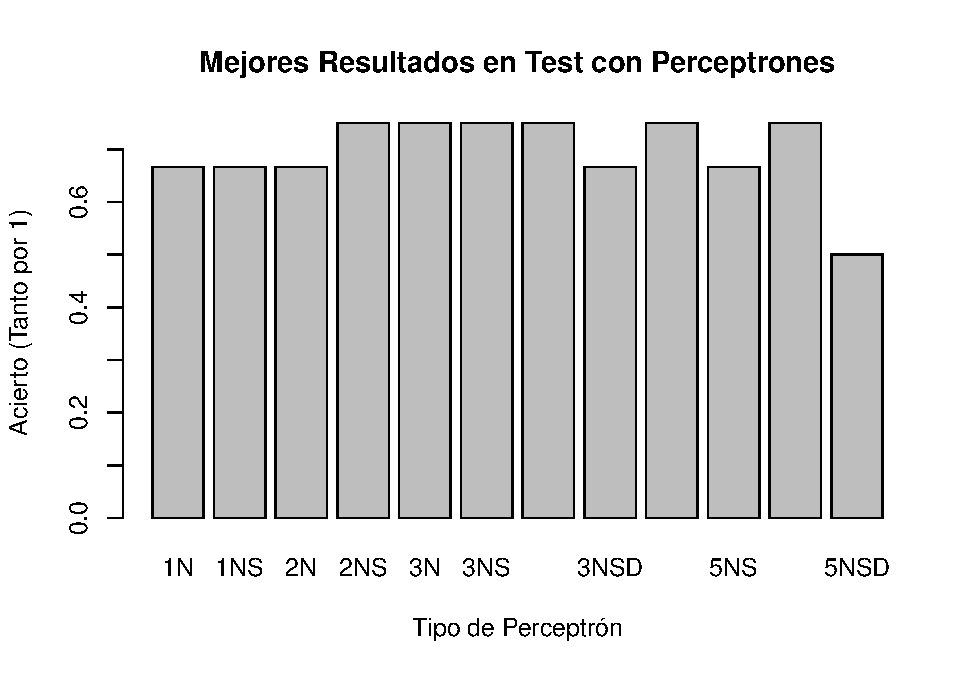
\includegraphics{codigo_files/figure-latex/analisis_resultados_perceptron-1.pdf}

Exporto a PDF este barplot:

\begin{Shaded}
\begin{Highlighting}[]
\KeywordTok{pdf}\NormalTok{(}\StringTok{"Imágenes Obtenidas/BarplotResultadosPerceptron.pdf"}\NormalTok{)}

\KeywordTok{barplot}\NormalTok{(array.maximos.perceptron,}
        \DataTypeTok{main =} \StringTok{"Mejores Resultados en Test con Perceptrones"}\NormalTok{,}
        \DataTypeTok{xlab =} \StringTok{"Tipo de Perceptrón",}
\StringTok{        ylab = "}\KeywordTok{Acierto}\NormalTok{ (Tanto por }\DecValTok{1}\NormalTok{)}\StringTok{",}
\StringTok{        names.arg = c("}\DecValTok{1}\NormalTok{ Neu}\StringTok{", "}\DecValTok{1}\NormalTok{ Neu Soft}\StringTok{", }
\StringTok{                      "}\DecValTok{2}\NormalTok{ Neu}\StringTok{", "}\DecValTok{2}\NormalTok{ Neu Soft}\StringTok{", }
\StringTok{                      "}\DecValTok{3}\NormalTok{ Neu}\StringTok{", "}\DecValTok{3}\NormalTok{ Neu Soft}\StringTok{", "}\DecValTok{3}\NormalTok{ Neu Decay}\StringTok{", "}\DecValTok{3}\NormalTok{ Neu Soft Decay}\StringTok{", }
\StringTok{                      "}\DecValTok{5}\NormalTok{ Neu}\StringTok{", "}\DecValTok{5}\NormalTok{ Neu Soft}\StringTok{", "}\DecValTok{5}\NormalTok{ Neu Decay}\StringTok{", "}\DecValTok{5}\NormalTok{ Neu Soft Decay}\StringTok{")}
\StringTok{      )}

\StringTok{dev.off}
\end{Highlighting}
\end{Shaded}

\begin{verbatim}
## function (which = dev.cur()) 
## {
##     if (which == 1) 
##         stop("cannot shut down device 1 (the null device)")
##     .External(C_devoff, as.integer(which))
##     dev.cur()
## }
## <bytecode: 0x0000000015754360>
## <environment: namespace:grDevices>
\end{verbatim}

\section{Obtención de Resultados de
Perceptrón}\label{obtencion-de-resultados-de-perceptron}

Importo los datos:

\begin{Shaded}
\begin{Highlighting}[]
\NormalTok{dataset.resultados <-}\StringTok{ }\KeywordTok{read.csv2}\NormalTok{(}\StringTok{"Datos/Resultados.txt"}\NormalTok{)}
\end{Highlighting}
\end{Shaded}

Ahora voy a sacar un gráfico interactivo donde comparo los resultados.

\begin{Shaded}
\begin{Highlighting}[]
\NormalTok{tipos =}\StringTok{ }\NormalTok{dataset.resultados[, }\DecValTok{1}\NormalTok{]}
\NormalTok{real =}\StringTok{ }\NormalTok{dataset.resultados[, }\DecValTok{2}\NormalTok{]}
\NormalTok{practico =}\StringTok{ }\NormalTok{dataset.resultados[, }\DecValTok{3}\NormalTok{]}

\NormalTok{p <-}\StringTok{ }\KeywordTok{plot_ly}\NormalTok{(dataset.resultados, }\DataTypeTok{x =} \OperatorTok{~}\NormalTok{tipos, }\DataTypeTok{y =} \OperatorTok{~}\NormalTok{real, }\DataTypeTok{type =} \StringTok{'bar'}\NormalTok{, }\DataTypeTok{name =} \StringTok{'Real'}\NormalTok{) }\OperatorTok\StringTok{ }\KeywordTok{add_trace}\NormalTok{(}\DataTypeTok{y =} \OperatorTok{~}\NormalTok{practico, }\DataTypeTok{name =} \StringTok{'Práctico'}\NormalTok{) }\OperatorTok\StringTok{ }\KeywordTok{layout}\NormalTok{(}\DataTypeTok{yaxis =} \KeywordTok{list}\NormalTok{(}\DataTypeTok{title =} \StringTok{'Porcentaje'}\NormalTok{), }\DataTypeTok{barmode =} \StringTok{'group'}\NormalTok{)}

\NormalTok{p }
\end{Highlighting}
\end{Shaded}

\hypertarget{htmlwidget-a81357ce590ddd8ee8c2}{}

\begin{Shaded}
\begin{Highlighting}[]
\CommentTok{#Mostramos el gráfico interactivo}
\end{Highlighting}
\end{Shaded}

Ahora que hemos sacado los resultados obtenidos con el perceptrón
multicapa, vamos con otras técnicas supervisadas:

\subsection{KNN}\label{knn}

Hacemos nuevos conjuntos:

\begin{Shaded}
\begin{Highlighting}[]
\CommentTok{# Para hacer la predicción con knn, voy a coger los grupos de una manera distinta:}

\NormalTok{conjuntoEntrenamiento =}\StringTok{ }\NormalTok{matriz.pacientes.datos.centscal[}\DecValTok{1}\OperatorTok{:}\DecValTok{55}\NormalTok{, }\DecValTok{1}\OperatorTok{:}\DecValTok{24}\NormalTok{]}
\NormalTok{conjuntoTest =}\StringTok{ }\NormalTok{matriz.pacientes.datos.centscal[}\DecValTok{56}\OperatorTok{:}\DecValTok{67}\NormalTok{, }\DecValTok{1}\OperatorTok{:}\DecValTok{24}\NormalTok{] }\CommentTok{# Utilizo por supuesto la matriz de centrado y escalado}

\NormalTok{etiquetasEntrenamiento =}\StringTok{ }\NormalTok{matriz.pacientes.etiquetas[}\DecValTok{1}\OperatorTok{:}\DecValTok{55}\NormalTok{, }\DecValTok{25}\NormalTok{]}
\NormalTok{etiquetasTest =}\StringTok{ }\NormalTok{matriz.pacientes.etiquetas[}\DecValTok{56}\OperatorTok{:}\DecValTok{67}\NormalTok{, }\DecValTok{25}\NormalTok{]}
\end{Highlighting}
\end{Shaded}

Si quisiéramos mostrar los conjuntos de entrenamiento y de test\ldots{}

\begin{Shaded}
\begin{Highlighting}[]
\NormalTok{conjuntoEntrenamiento}
\NormalTok{conjuntoTest}
\NormalTok{etiquetasEntrenamiento}
\NormalTok{etiquetasTest}
\end{Highlighting}
\end{Shaded}

Comenzamos las pruebas. Como sabemos, normalmente el mejor valor de K
para KNN suele ser el valor que más se acerque a la raíz cuadrada del
total de los valores. Por eso, empezaremos por K = 8:

\subsubsection{Para K = 8\ldots{}}\label{para-k-8}

\begin{Shaded}
\begin{Highlighting}[]
\KeywordTok{set.seed}\NormalTok{(}\DecValTok{2}\NormalTok{)}

\NormalTok{prediccion.knn.}\DecValTok{8}\NormalTok{ <-}\StringTok{ }\KeywordTok{knn}\NormalTok{(}\DataTypeTok{train =}\NormalTok{ conjuntoEntrenamiento, }\DataTypeTok{test =}\NormalTok{ conjuntoTest, }\DataTypeTok{cl =}\NormalTok{ etiquetasEntrenamiento, }\DataTypeTok{k =} \DecValTok{8}\NormalTok{)}
\NormalTok{prediccion.knn.}\DecValTok{8}
\end{Highlighting}
\end{Shaded}

\begin{verbatim}
##  [1] 1 2 2 1 2 1 2 2 2 1 2 2
## Levels: 1 2 3 4
\end{verbatim}

Sacamos crosstable:

\begin{Shaded}
\begin{Highlighting}[]
\KeywordTok{CrossTable}\NormalTok{(}\DataTypeTok{x =}\NormalTok{ etiquetasTest , }\DataTypeTok{y =}\NormalTok{ prediccion.knn.}\DecValTok{8}\NormalTok{, }\DataTypeTok{prop.chisq =} \OtherTok{FALSE}\NormalTok{)}
\end{Highlighting}
\end{Shaded}

\begin{verbatim}
## 
##  
##    Cell Contents
## |-------------------------|
## |                       N |
## |           N / Row Total |
## |           N / Col Total |
## |         N / Table Total |
## |-------------------------|
## 
##  
## Total Observations in Table:  12 
## 
##  
##               | prediccion.knn.8 
## etiquetasTest |         1 |         2 | Row Total | 
## --------------|-----------|-----------|-----------|
##             1 |         1 |         3 |         4 | 
##               |     0.250 |     0.750 |     0.333 | 
##               |     0.250 |     0.375 |           | 
##               |     0.083 |     0.250 |           | 
## --------------|-----------|-----------|-----------|
##             2 |         1 |         3 |         4 | 
##               |     0.250 |     0.750 |     0.333 | 
##               |     0.250 |     0.375 |           | 
##               |     0.083 |     0.250 |           | 
## --------------|-----------|-----------|-----------|
##             3 |         0 |         2 |         2 | 
##               |     0.000 |     1.000 |     0.167 | 
##               |     0.000 |     0.250 |           | 
##               |     0.000 |     0.167 |           | 
## --------------|-----------|-----------|-----------|
##             4 |         2 |         0 |         2 | 
##               |     1.000 |     0.000 |     0.167 | 
##               |     0.500 |     0.000 |           | 
##               |     0.167 |     0.000 |           | 
## --------------|-----------|-----------|-----------|
##  Column Total |         4 |         8 |        12 | 
##               |     0.333 |     0.667 |           | 
## --------------|-----------|-----------|-----------|
## 
## 
\end{verbatim}

\subsubsection{Para K = 6}\label{para-k-6}

\begin{Shaded}
\begin{Highlighting}[]
\KeywordTok{set.seed}\NormalTok{(}\DecValTok{2}\NormalTok{)}

\NormalTok{prediccion.knn.}\DecValTok{6}\NormalTok{ <-}\StringTok{ }\KeywordTok{knn}\NormalTok{(}\DataTypeTok{train =}\NormalTok{ conjuntoEntrenamiento, }\DataTypeTok{test =}\NormalTok{ conjuntoTest, }\DataTypeTok{cl =}\NormalTok{ etiquetasEntrenamiento, }\DataTypeTok{k =} \DecValTok{6}\NormalTok{)}
\NormalTok{prediccion.knn.}\DecValTok{6}
\end{Highlighting}
\end{Shaded}

\begin{verbatim}
##  [1] 4 2 2 1 2 1 2 2 2 1 2 2
## Levels: 1 2 3 4
\end{verbatim}

Obtenemos la crosstable:

\begin{Shaded}
\begin{Highlighting}[]
\KeywordTok{CrossTable}\NormalTok{(}\DataTypeTok{x =}\NormalTok{ etiquetasTest , }\DataTypeTok{y =}\NormalTok{ prediccion.knn.}\DecValTok{6}\NormalTok{, }\DataTypeTok{prop.chisq =} \OtherTok{FALSE}\NormalTok{)}
\end{Highlighting}
\end{Shaded}

\begin{verbatim}
## 
##  
##    Cell Contents
## |-------------------------|
## |                       N |
## |           N / Row Total |
## |           N / Col Total |
## |         N / Table Total |
## |-------------------------|
## 
##  
## Total Observations in Table:  12 
## 
##  
##               | prediccion.knn.6 
## etiquetasTest |         1 |         2 |         4 | Row Total | 
## --------------|-----------|-----------|-----------|-----------|
##             1 |         0 |         3 |         1 |         4 | 
##               |     0.000 |     0.750 |     0.250 |     0.333 | 
##               |     0.000 |     0.375 |     1.000 |           | 
##               |     0.000 |     0.250 |     0.083 |           | 
## --------------|-----------|-----------|-----------|-----------|
##             2 |         1 |         3 |         0 |         4 | 
##               |     0.250 |     0.750 |     0.000 |     0.333 | 
##               |     0.333 |     0.375 |     0.000 |           | 
##               |     0.083 |     0.250 |     0.000 |           | 
## --------------|-----------|-----------|-----------|-----------|
##             3 |         0 |         2 |         0 |         2 | 
##               |     0.000 |     1.000 |     0.000 |     0.167 | 
##               |     0.000 |     0.250 |     0.000 |           | 
##               |     0.000 |     0.167 |     0.000 |           | 
## --------------|-----------|-----------|-----------|-----------|
##             4 |         2 |         0 |         0 |         2 | 
##               |     1.000 |     0.000 |     0.000 |     0.167 | 
##               |     0.667 |     0.000 |     0.000 |           | 
##               |     0.167 |     0.000 |     0.000 |           | 
## --------------|-----------|-----------|-----------|-----------|
##  Column Total |         3 |         8 |         1 |        12 | 
##               |     0.250 |     0.667 |     0.083 |           | 
## --------------|-----------|-----------|-----------|-----------|
## 
## 
\end{verbatim}

\subsubsection{Para k = 10}\label{para-k-10}

\begin{Shaded}
\begin{Highlighting}[]
\KeywordTok{set.seed}\NormalTok{(}\DecValTok{2}\NormalTok{)}

\NormalTok{prediccion.knn.}\DecValTok{10}\NormalTok{ <-}\StringTok{ }\KeywordTok{knn}\NormalTok{(}\DataTypeTok{train =}\NormalTok{ conjuntoEntrenamiento, }\DataTypeTok{test =}\NormalTok{ conjuntoTest, }\DataTypeTok{cl =}\NormalTok{ etiquetasEntrenamiento, }\DataTypeTok{k =} \DecValTok{10}\NormalTok{)}
\NormalTok{prediccion.knn.}\DecValTok{10}
\end{Highlighting}
\end{Shaded}

\begin{verbatim}
##  [1] 1 2 2 1 2 1 2 2 4 1 2 2
## Levels: 1 2 3 4
\end{verbatim}

Obtenemos la crosstable:

\begin{Shaded}
\begin{Highlighting}[]
\KeywordTok{CrossTable}\NormalTok{(}\DataTypeTok{x =}\NormalTok{ etiquetasTest , }\DataTypeTok{y =}\NormalTok{ prediccion.knn.}\DecValTok{10}\NormalTok{, }\DataTypeTok{prop.chisq =} \OtherTok{FALSE}\NormalTok{)}
\end{Highlighting}
\end{Shaded}

\begin{verbatim}
## 
##  
##    Cell Contents
## |-------------------------|
## |                       N |
## |           N / Row Total |
## |           N / Col Total |
## |         N / Table Total |
## |-------------------------|
## 
##  
## Total Observations in Table:  12 
## 
##  
##               | prediccion.knn.10 
## etiquetasTest |         1 |         2 |         4 | Row Total | 
## --------------|-----------|-----------|-----------|-----------|
##             1 |         1 |         3 |         0 |         4 | 
##               |     0.250 |     0.750 |     0.000 |     0.333 | 
##               |     0.250 |     0.429 |     0.000 |           | 
##               |     0.083 |     0.250 |     0.000 |           | 
## --------------|-----------|-----------|-----------|-----------|
##             2 |         1 |         2 |         1 |         4 | 
##               |     0.250 |     0.500 |     0.250 |     0.333 | 
##               |     0.250 |     0.286 |     1.000 |           | 
##               |     0.083 |     0.167 |     0.083 |           | 
## --------------|-----------|-----------|-----------|-----------|
##             3 |         0 |         2 |         0 |         2 | 
##               |     0.000 |     1.000 |     0.000 |     0.167 | 
##               |     0.000 |     0.286 |     0.000 |           | 
##               |     0.000 |     0.167 |     0.000 |           | 
## --------------|-----------|-----------|-----------|-----------|
##             4 |         2 |         0 |         0 |         2 | 
##               |     1.000 |     0.000 |     0.000 |     0.167 | 
##               |     0.500 |     0.000 |     0.000 |           | 
##               |     0.167 |     0.000 |     0.000 |           | 
## --------------|-----------|-----------|-----------|-----------|
##  Column Total |         4 |         7 |         1 |        12 | 
##               |     0.333 |     0.583 |     0.083 |           | 
## --------------|-----------|-----------|-----------|-----------|
## 
## 
\end{verbatim}

\subsubsection{Como se puede observar, la mejor predicción la hemos
hecho con K =
8}\label{como-se-puede-observar-la-mejor-prediccion-la-hemos-hecho-con-k-8}

\subsection{Random Forest}\label{random-forest}

Ahora voy a implementar una solución mediante Random Forest:

\begin{Shaded}
\begin{Highlighting}[]
\KeywordTok{set.seed}\NormalTok{(}\DecValTok{3}\NormalTok{) }\CommentTok{#Pongo una seed para reproducibilidad}
\end{Highlighting}
\end{Shaded}

Una vez instalado e importado, lo que tengo que hacer es crear el Random
Forest, y ejecutarlo\ldots{}

\begin{Shaded}
\begin{Highlighting}[]
\NormalTok{model <-}\StringTok{ }\KeywordTok{randomForest}\NormalTok{(}\KeywordTok{as.factor}\NormalTok{(dataset[, }\DecValTok{26}\NormalTok{]) }\OperatorTok{~}\StringTok{ }\NormalTok{., }\DataTypeTok{data =}\NormalTok{ dataset[, }\DecValTok{2}\OperatorTok{:}\DecValTok{25}\NormalTok{], }\DataTypeTok{importance =} \OtherTok{TRUE}\NormalTok{, }\DataTypeTok{ntree =} \DecValTok{300}\NormalTok{)}
\NormalTok{model}
\end{Highlighting}
\end{Shaded}

\begin{verbatim}
## 
## Call:
##  randomForest(formula = as.factor(dataset[, 26]) ~ ., data = dataset[,      2:25], importance = TRUE, ntree = 300) 
##                Type of random forest: classification
##                      Number of trees: 300
## No. of variables tried at each split: 4
## 
##         OOB estimate of  error rate: 50.75%
## Confusion matrix:
##   1  2 3 4 class.error
## 1 5  9 1 2   0.7058824
## 2 4 26 0 0   0.1333333
## 3 2  5 0 1   1.0000000
## 4 7  3 0 2   0.8333333
\end{verbatim}

Aquí podemos ver la matriz de confusión, de la que obtenemos también el
fallo por clases.

El Out-Of-Bag es un método de estimación de error que se usa en algunos
algoritmos como Random Forest, y usa el modelo de Bagging para hacer
muestras de submuestras usadas para el entrenamiento. El OOB es el error
de predidcción medio de cada una de las muestras de entrenamiento.

Bagging es un meta-algoritmo usado para aumentar la estabilidad y
precisión de algoritmos de Machine Learning de clasificación y
regresión.

Vemos que el valor OOB (Out-Of-the-Bag) es una valor muy alto, de
alrededor del 50\%, por lo que nuestro modelo no está prediciendo bien.

Ahora obtenemos el número de árboles que necesitamos realmente, y la
importancia de las variables en este modelo:

\begin{Shaded}
\begin{Highlighting}[]
\KeywordTok{plot}\NormalTok{(model, }\DataTypeTok{main=}\StringTok{"Random Forest"}\NormalTok{)}
\end{Highlighting}
\end{Shaded}

\includegraphics{codigo_files/figure-latex/importance_graphs_RF-1.pdf}

\begin{Shaded}
\begin{Highlighting}[]
\KeywordTok{varImpPlot}\NormalTok{(model, }\DataTypeTok{main =} \StringTok{"Random Forest - MDA y Gini"}\NormalTok{) }\CommentTok{# Gracias a importance = true}
\end{Highlighting}
\end{Shaded}

\includegraphics{codigo_files/figure-latex/importance_graphs_RF-2.pdf}

Exporto a PDF los gráficos obtenidos:

\begin{Shaded}
\begin{Highlighting}[]
\KeywordTok{pdf}\NormalTok{(}\StringTok{"Imágenes Obtenidas/ResultadosRandomForest.pdf"}\NormalTok{)}

\KeywordTok{plot}\NormalTok{(model, }\DataTypeTok{main=}\StringTok{"Random Forest"}\NormalTok{)}
\KeywordTok{varImpPlot}\NormalTok{(model, }\DataTypeTok{main =} \StringTok{"Random Forest - MDA y Gini"}\NormalTok{)}

\NormalTok{dev.off}
\end{Highlighting}
\end{Shaded}

\begin{verbatim}
## function (which = dev.cur()) 
## {
##     if (which == 1) 
##         stop("cannot shut down device 1 (the null device)")
##     .External(C_devoff, as.integer(which))
##     dev.cur()
## }
## <bytecode: 0x0000000015754360>
## <environment: namespace:grDevices>
\end{verbatim}

Vamos a interpretar estos datos del modelo:

\begin{itemize}
\item
  MeanDecreaseAccuracy se refiere al decremento de la exactitud del
  modelo si se permutan los valores en cada característica. En otras
  palabras, MDA nos muestra la media de valores que se clasificarían mal
  si se quitara esa característica de la predicción. Por ello, eliminar
  elementos coo la impulsividad o la pseudo-resiliencia sería fatal para
  el modelo, mientras que la eliminación de relación con el contexto
  mala, pensamiento dicotómico o generalización excesiva parece ser que
  mejorarían el sistema.
\item
  MeanDecreaseGini se refiere a la medida de la ganancia media de pureza
  mediante la división de cierta variable. Cuanto más importante sea la
  variable, habrá un mayor descenso en el Gini. La importancia de este
  está íntimamente relacionada a la función de decisión local, que
  Random Forest usa para seleccionar cual es la mejor separación. Debido
  a esto, estamos viendo que la edad, la impulsividad y la
  pseudo-responsabilidad son valores que tienen un gran descenso en
  Gini, lo cual significa que Random Forest ha determinado que eran de
  gran importancia.
\end{itemize}

Un elemento que me gustaría destacar es que el modelo está bastante
regularizado y es bastante robusto, ya que casi todas las variables son
bastante resistentes a las permutaciones, y por lo tanto no tienen un
peso extremo a la hora de tomar decisiones, a excepción de la
impulsividad.

Ahora, para probar a ver si hay diferencia, en vez del dataset normal
voy a usar el dataset centrado y escalado, para ver si el OOB desciende:

\begin{Shaded}
\begin{Highlighting}[]
\CommentTok{# primero añado el grupo a la matriz, creando una nueva}

\NormalTok{matriz.pacientes.datos.centscal.grupo <-}\StringTok{ }\KeywordTok{cbind}\NormalTok{(matriz.pacientes.datos.centscal, dataset}\OperatorTok{$}\NormalTok{grupo)}
\KeywordTok{colnames}\NormalTok{(matriz.pacientes.datos.centscal.grupo)[}\DecValTok{25}\NormalTok{] <-}\StringTok{ "grupo"}
\end{Highlighting}
\end{Shaded}

Ahora entrenamos el nuevo modelo:

\begin{Shaded}
\begin{Highlighting}[]
\KeywordTok{set.seed}\NormalTok{(}\DecValTok{3}\NormalTok{)}

\NormalTok{model_centscal <-}\StringTok{ }\KeywordTok{randomForest}\NormalTok{(}\KeywordTok{as.factor}\NormalTok{(grupo) }\OperatorTok{~}\StringTok{ }\NormalTok{., }\DataTypeTok{data =}\NormalTok{ matriz.pacientes.datos.centscal.grupo, }\DataTypeTok{importance =} \OtherTok{TRUE}\NormalTok{, }\DataTypeTok{ntree =} \DecValTok{200}\NormalTok{)}
\NormalTok{model_centscal}
\end{Highlighting}
\end{Shaded}

\begin{verbatim}
## 
## Call:
##  randomForest(formula = as.factor(grupo) ~ ., data = matriz.pacientes.datos.centscal.grupo,      importance = TRUE, ntree = 200) 
##                Type of random forest: classification
##                      Number of trees: 200
## No. of variables tried at each split: 4
## 
##         OOB estimate of  error rate: 49.25%
## Confusion matrix:
##   1  2 3 4 class.error
## 1 5  9 1 2   0.7058824
## 2 4 26 0 0   0.1333333
## 3 2  5 0 1   1.0000000
## 4 6  3 0 3   0.7500000
\end{verbatim}

Podemos ver que obtenemos lo mismo. Vamos a ver si también obtenemos lo
mismo en los grafos de importancia:

\begin{Shaded}
\begin{Highlighting}[]
\KeywordTok{plot}\NormalTok{(model_centscal, }\DataTypeTok{main=}\StringTok{"Random Forest Con Centrado y Escalado"}\NormalTok{)}
\end{Highlighting}
\end{Shaded}

\includegraphics{codigo_files/figure-latex/importance_graphs_RF_centscal-1.pdf}

\begin{Shaded}
\begin{Highlighting}[]
\KeywordTok{varImpPlot}\NormalTok{(model_centscal, }\DataTypeTok{main=}\StringTok{"Random Forest con Centrado y Escalado - MDA y Gini"}\NormalTok{) }\CommentTok{# Gracias a importance = true}
\end{Highlighting}
\end{Shaded}

\includegraphics{codigo_files/figure-latex/importance_graphs_RF_centscal-2.pdf}

Exporto a PDF estos resultados:

\begin{Shaded}
\begin{Highlighting}[]
\CommentTok{# Lo exporto de nuevo a PDF}

\KeywordTok{pdf}\NormalTok{(}\StringTok{"Imágenes Obtenidas/ResultadosRandomForestCentScal.pdf"}\NormalTok{)}

\KeywordTok{plot}\NormalTok{(model_centscal, }\DataTypeTok{main=}\StringTok{"Random Forest Con Centrado y Escalado"}\NormalTok{)}
\KeywordTok{varImpPlot}\NormalTok{(model_centscal, }\DataTypeTok{main=}\StringTok{"Random Forest con Centrado y Escalado - MDA y Gini"}\NormalTok{)}

\NormalTok{dev.off}
\end{Highlighting}
\end{Shaded}

\begin{verbatim}
## function (which = dev.cur()) 
## {
##     if (which == 1) 
##         stop("cannot shut down device 1 (the null device)")
##     .External(C_devoff, as.integer(which))
##     dev.cur()
## }
## <bytecode: 0x0000000015754360>
## <environment: namespace:grDevices>
\end{verbatim}

En este caso, el MDA me dice que el sexo es la gran lacra de este
modelo, mientras que la impulsividad sigue siendo el factor más
determinante para acertar. Del Gini obtengo resultados similares.

Ahora, ya que hemos visto que cambiando el dataset no mejoramos el
modelo, lo que vamos a hacer es, con el primer dataset, quitar las
columnas que en el MDA tengan un valor negativo, de tal manera que la
precisión del modelo debería de aumentar.

\begin{Shaded}
\begin{Highlighting}[]
\CommentTok{# Las columnas que son una mayor lacra son las siguientes: Relación Contexto Mala, Pensamiento dicotómico, generalización excesiva, sexo, razonamiento emocional, deberías, asertivo, relación-contexto buena, etiquetado, relación contexto trauma.}

\NormalTok{dataset.randomforest <-}\StringTok{ }\NormalTok{dataset[ , }\KeywordTok{c}\NormalTok{(}\OperatorTok{-}\DecValTok{1}\NormalTok{, }\OperatorTok{-}\DecValTok{3}\NormalTok{, }\OperatorTok{-}\DecValTok{4}\NormalTok{, }\OperatorTok{-}\DecValTok{5}\NormalTok{, }\OperatorTok{-}\DecValTok{6}\NormalTok{, }\OperatorTok{-}\DecValTok{13}\NormalTok{, }\OperatorTok{-}\DecValTok{14}\NormalTok{, }\OperatorTok{-}\DecValTok{15}\NormalTok{, }\OperatorTok{-}\DecValTok{20}\NormalTok{, }\OperatorTok{-}\DecValTok{23}\NormalTok{)]}
\KeywordTok{head}\NormalTok{(dataset.randomforest)}
\end{Highlighting}
\end{Shaded}

\begin{verbatim}
##   edad ed_perm ed_norm ed_estr resil_ba resil_me resil_al fil_men max_min conc_arb pseu_res raz_emo
## 1   20       0       1       0        0        1        0       0       1        1        0       1
## 2   19       0       0       1        1        0        0       0       1        1        1       0
## 3   23       1       0       0        1        0        0       0       1        1        0       1
## 4   16       1       0       0        1        0        0       1       1        1        0       1
## 5   23       0       0       1        0        1        0       1       1        1        1       1
## 6   22       0       1       0        1        0        0       0       1        1        0       1
##   inhib agres impuls grupo
## 1     0     1      1     1
## 2     1     0      0     2
## 3     1     0      0     2
## 4     0     1      1     4
## 5     1     0      0     2
## 6     1     0      1     4
\end{verbatim}

Ahora que tenemos el dataset creado, vamos a hacer la predicción de
nuevo:

\begin{Shaded}
\begin{Highlighting}[]
\KeywordTok{set.seed}\NormalTok{(}\DecValTok{3}\NormalTok{)}

\NormalTok{model_new <-}\StringTok{ }\KeywordTok{randomForest}\NormalTok{(}\KeywordTok{as.factor}\NormalTok{(grupo) }\OperatorTok{~}\StringTok{ }\NormalTok{., }\DataTypeTok{data =}\NormalTok{ dataset.randomforest, }\DataTypeTok{importance =} \OtherTok{TRUE}\NormalTok{, }\DataTypeTok{ntree =} \DecValTok{200}\NormalTok{)}
\NormalTok{model_new}
\end{Highlighting}
\end{Shaded}

\begin{verbatim}
## 
## Call:
##  randomForest(formula = as.factor(grupo) ~ ., data = dataset.randomforest,      importance = TRUE, ntree = 200) 
##                Type of random forest: classification
##                      Number of trees: 200
## No. of variables tried at each split: 3
## 
##         OOB estimate of  error rate: 46.27%
## Confusion matrix:
##   1  2 3 4 class.error
## 1 4  9 0 4   0.7647059
## 2 2 27 0 1   0.1000000
## 3 2  5 0 1   1.0000000
## 4 4  3 0 5   0.5833333
\end{verbatim}

Vamos a ver ahora ls gráficos\ldots{}

\begin{Shaded}
\begin{Highlighting}[]
\KeywordTok{plot}\NormalTok{(model_new, }\DataTypeTok{main=}\StringTok{"Random Forest Nuevo"}\NormalTok{)}
\end{Highlighting}
\end{Shaded}

\includegraphics{codigo_files/figure-latex/importance_graphs_RF_new-1.pdf}

\begin{Shaded}
\begin{Highlighting}[]
\KeywordTok{varImpPlot}\NormalTok{(model_new, }\DataTypeTok{main =} \StringTok{"Random Forest Nuevo - MDA y Gini"}\NormalTok{) }
\end{Highlighting}
\end{Shaded}

\includegraphics{codigo_files/figure-latex/importance_graphs_RF_new-2.pdf}

Exporto a PDF estos resultados del Random Forest corregido:

\begin{Shaded}
\begin{Highlighting}[]
\KeywordTok{pdf}\NormalTok{(}\StringTok{"Imágenes Obtenidas/ResultadosRandomForestMejorado.pdf"}\NormalTok{)}

\KeywordTok{plot}\NormalTok{(model_new, }\DataTypeTok{main=}\StringTok{"Random Forest Nuevo"}\NormalTok{)}
\KeywordTok{varImpPlot}\NormalTok{(model_new, }\DataTypeTok{main =} \StringTok{"Random Forest Nuevo - MDA y Gini"}\NormalTok{) }

\NormalTok{dev.off}
\end{Highlighting}
\end{Shaded}

\begin{verbatim}
## function (which = dev.cur()) 
## {
##     if (which == 1) 
##         stop("cannot shut down device 1 (the null device)")
##     .External(C_devoff, as.integer(which))
##     dev.cur()
## }
## <bytecode: 0x0000000015754360>
## <environment: namespace:grDevices>
\end{verbatim}

Como se puede observar, ahora hay nuevas variables que ``lastran'' el
resultado del Random Forest. De todas maneras, hemos conseguido una
bajada del 50\% de media en OOB Error al 45\% de media en OOB Error
(entrenando), lo cual es una disminución menos notable de lo esperado,
pero es una disminución.

Ahora lo voy a hacer con 10 fold X Validation:

\begin{Shaded}
\begin{Highlighting}[]
\KeywordTok{set.seed}\NormalTok{(}\DecValTok{4}\NormalTok{)}

\NormalTok{result <-}\StringTok{ }\KeywordTok{rfcv}\NormalTok{(dataset[, }\DecValTok{2}\OperatorTok{:}\DecValTok{26}\NormalTok{], }\KeywordTok{as.factor}\NormalTok{(dataset}\OperatorTok{$}\NormalTok{grupo), }\DataTypeTok{cv.fold=}\DecValTok{10}\NormalTok{)}
\KeywordTok{head}\NormalTok{(result)}
\end{Highlighting}
\end{Shaded}

\begin{verbatim}
## $n.var
## [1] 25 12  6  3  1
## 
## $error.cv
##        25        12         6         3         1 
## 0.1940299 0.1492537 0.1194030 0.1343284 0.0000000 
## 
## $predicted
## $predicted$`25`
##  [1] 2 2 2 4 2 4 2 2 2 2 2 1 2 1 2 4 2 2 2 2 2 2 1 4 1 2 4 4 2 2 2 4 2 2 2 2 2 4 2 1 2 1 1 2 2 2 4 2
## [49] 1 2 4 1 2 2 1 1 2 1 4 2 1 1 3 2 4 2 1
## Levels: 1 2 3 4
## 
## $predicted$`12`
##  [1] 1 2 2 4 2 4 2 1 2 2 2 1 2 1 1 4 4 2 2 2 2 2 1 4 1 2 4 4 2 2 2 4 2 2 2 2 2 4 2 1 2 1 1 2 2 2 4 2
## [49] 1 2 4 1 2 3 1 1 2 1 4 2 1 2 2 2 4 2 1
## Levels: 1 2 3 4
## 
## $predicted$`6`
##  [1] 1 2 2 4 2 4 2 1 2 2 2 1 2 1 1 4 2 2 2 2 2 2 1 4 1 3 4 4 2 2 2 4 2 2 2 2 2 4 2 1 2 1 1 2 2 2 4 2
## [49] 1 2 4 1 2 3 1 1 2 1 4 2 1 1 3 2 4 2 1
## Levels: 1 2 3 4
## 
## $predicted$`3`
##  [1] 1 2 2 4 2 4 2 1 2 2 2 1 2 1 1 4 4 2 2 2 2 2 1 4 1 2 4 4 2 2 2 2 2 2 2 2 2 2 2 1 2 1 1 2 2 2 4 2
## [49] 1 2 4 1 2 2 1 1 2 1 4 2 2 1 2 2 4 2 1
## Levels: 1 2 3 4
## 
## $predicted$`1`
##  [1] 1 2 2 4 2 4 4 1 2 2 2 1 2 1 1 4 4 2 2 2 2 3 1 4 1 3 4 4 2 2 2 3 2 2 2 2 2 3 2 1 3 1 1 2 2 2 4 2
## [49] 1 2 4 1 2 3 1 1 3 1 4 2 2 1 3 2 4 2 1
## Levels: 1 2 3 4
\end{verbatim}

Podemos ver el error, bajo la variable \$error.cv, y podemos ver las
predicciones que se han hecho para cada una de las n.var.

\subsection{SVM de Kernel Lineal}\label{svm-de-kernel-lineal}

Lo bueno que tiene SVM es que es muy robusto frente a la dimensión, por
lo que deberíamos de obtener a priori buenos resultados con este método.

Con este método no necesito tener un conjunto de entrenaminento y otro
de test, por lo que sigo adelante.

Ahora que hemos instalado la librería, vamos a crear el SVM:

\begin{Shaded}
\begin{Highlighting}[]
\KeywordTok{set.seed}\NormalTok{(}\DecValTok{5}\NormalTok{)}

\NormalTok{modelo.svm <-}\StringTok{ }\KeywordTok{svm}\NormalTok{(matriz.pacientes.datos.centscal, }\KeywordTok{as.factor}\NormalTok{(dataset[, }\DecValTok{26}\NormalTok{]), }\DataTypeTok{kernel =} \StringTok{"linear"}\NormalTok{) }\CommentTok{# Al poner los grupos como factor, estoy consiguiendo que no sean continuos para el modelo, sino "discretos", ya que los factor no son valores que puedan ser continuos. Con esto consigo una clasificación.}
\KeywordTok{summary}\NormalTok{(modelo.svm)}
\end{Highlighting}
\end{Shaded}

\begin{verbatim}
## 
## Call:
## svm.default(x = matriz.pacientes.datos.centscal, y = as.factor(dataset[, 26]), kernel = "linear")
## 
## 
## Parameters:
##    SVM-Type:  C-classification 
##  SVM-Kernel:  linear 
##        cost:  1 
##       gamma:  0.04166667 
## 
## Number of Support Vectors:  58
## 
##  ( 16 22 12 8 )
## 
## 
## Number of Classes:  4 
## 
## Levels: 
##  1 2 3 4
\end{verbatim}

Como vemos en el resumen, tenemos una C-Classification (necesitamos
clasificar), con kernel lineal, y 58 vectores soporte.

Ahora que tenemos creado este primer modelo, toca predecir:

\begin{Shaded}
\begin{Highlighting}[]
\KeywordTok{set.seed}\NormalTok{(}\DecValTok{5}\NormalTok{)}

\NormalTok{prediccion <-}\StringTok{ }\KeywordTok{predict}\NormalTok{(modelo.svm, matriz.pacientes.datos.centscal)}
\NormalTok{prediccion}
\end{Highlighting}
\end{Shaded}

\begin{verbatim}
##  1  2  3  4  5  6  7  8  9 10 11 12 13 14 15 16 17 18 19 20 21 22 23 24 25 26 27 28 29 30 31 32 33 
##  1  2  2  4  2  4  4  2  2  2  2  1  2  1  3  4  2  2  2  2  2  3  1  1  1  3  4  4  2  2  2  1  2 
## 34 35 36 37 38 39 40 41 42 43 44 45 46 47 48 49 50 51 52 53 54 55 56 57 58 59 60 61 62 63 64 65 66 
##  2  2  2  2  3  2  1  3  1  1  1  2  2  2  2  4  2  1  1  2  3  1  1  3  1  4  2  4  2  3  2  4  2 
## 67 
##  1 
## Levels: 1 2 3 4
\end{verbatim}

Ahora que hemos predicho, tenemos que sacar la matriz de confusión:

\begin{Shaded}
\begin{Highlighting}[]
\NormalTok{matriz.conf <-}\StringTok{ }\KeywordTok{table}\NormalTok{(prediccion, dataset[ ,}\DecValTok{26}\NormalTok{])}
\NormalTok{matriz.conf}
\end{Highlighting}
\end{Shaded}

\begin{verbatim}
##           
## prediccion  1  2  3  4
##          1 13  1  1  2
##          2  2 28  0  2
##          3  1  0  7  0
##          4  1  1  0  8
\end{verbatim}

\begin{Shaded}
\begin{Highlighting}[]
\KeywordTok{sum}\NormalTok{(}\KeywordTok{diag}\NormalTok{(matriz.conf))}\OperatorTok{/}\DecValTok{67}
\end{Highlighting}
\end{Shaded}

\begin{verbatim}
## [1] 0.8358209
\end{verbatim}

\subsection{SVM de Kernel RBF}\label{svm-de-kernel-rbf}

\begin{Shaded}
\begin{Highlighting}[]
\KeywordTok{set.seed}\NormalTok{(}\DecValTok{5}\NormalTok{)}

\NormalTok{modelo_svm.radial <-}\StringTok{ }\KeywordTok{svm}\NormalTok{(matriz.pacientes.datos.centscal, }\KeywordTok{as.factor}\NormalTok{(dataset[, }\DecValTok{26}\NormalTok{]), }\DataTypeTok{kernel=}\StringTok{"radial"}\NormalTok{)}
\KeywordTok{summary}\NormalTok{(modelo_svm.radial)}
\end{Highlighting}
\end{Shaded}

\begin{verbatim}
## 
## Call:
## svm.default(x = matriz.pacientes.datos.centscal, y = as.factor(dataset[, 26]), kernel = "radial")
## 
## 
## Parameters:
##    SVM-Type:  C-classification 
##  SVM-Kernel:  radial 
##        cost:  1 
##       gamma:  0.04166667 
## 
## Number of Support Vectors:  66
## 
##  ( 17 29 12 8 )
## 
## 
## Number of Classes:  4 
## 
## Levels: 
##  1 2 3 4
\end{verbatim}

Aquí tenemos una C-Classification (necesaria para clasificar), con
Kernel esta vez radial y 66 vectores soporte.

Ahora que tenemos creado este primer modelo, toca predecir:

\begin{Shaded}
\begin{Highlighting}[]
\KeywordTok{set.seed}\NormalTok{(}\DecValTok{5}\NormalTok{)}

\NormalTok{prediccion.radial <-}\StringTok{ }\KeywordTok{predict}\NormalTok{(modelo_svm.radial, matriz.pacientes.datos.centscal)}
\NormalTok{prediccion.radial}
\end{Highlighting}
\end{Shaded}

\begin{verbatim}
##  1  2  3  4  5  6  7  8  9 10 11 12 13 14 15 16 17 18 19 20 21 22 23 24 25 26 27 28 29 30 31 32 33 
##  1  2  2  4  2  4  2  2  2  2  2  1  2  1  2  4  2  2  2  2  2  2  1  1  1  2  4  2  2  2  2  2  2 
## 34 35 36 37 38 39 40 41 42 43 44 45 46 47 48 49 50 51 52 53 54 55 56 57 58 59 60 61 62 63 64 65 66 
##  2  2  2  2  1  2  1  2  1  1  2  2  2  2  2  1  2  1  1  2  3  1  1  2  1  4  2  1  2  2  2  4  2 
## 67 
##  2 
## Levels: 1 2 3 4
\end{verbatim}

Ahora que hemos predicho, tenemos que sacar la matriz de confusión:

\begin{Shaded}
\begin{Highlighting}[]
\NormalTok{matriz.conf.radial <-}\StringTok{ }\KeywordTok{table}\NormalTok{(prediccion.radial, dataset[,}\DecValTok{26}\NormalTok{])}
\NormalTok{matriz.conf.radial}
\end{Highlighting}
\end{Shaded}

\begin{verbatim}
##                  
## prediccion.radial  1  2  3  4
##                 1 13  1  1  2
##                 2  4 29  6  4
##                 3  0  0  1  0
##                 4  0  0  0  6
\end{verbatim}

\begin{Shaded}
\begin{Highlighting}[]
\KeywordTok{sum}\NormalTok{(}\KeywordTok{diag}\NormalTok{(matriz.conf.radial))}\OperatorTok{/}\DecValTok{67}
\end{Highlighting}
\end{Shaded}

\begin{verbatim}
## [1] 0.7313433
\end{verbatim}

\subsubsection{Como vemos, nos movemos en valores superiores al 75\% de
acierto}\label{como-vemos-nos-movemos-en-valores-superiores-al-75-de-acierto}

Por lo tanto, SVM es una buena técnica para la predicción en este
problema.

\begin{center}\rule{0.5\linewidth}{\linethickness}\end{center}

Ahora pasamos a los modelos de inteligencia artificial no supervisados:

\section{Modelos de inteligencia artificial no
supervisados}\label{modelos-de-inteligencia-artificial-no-supervisados}

El primer modelo de inteligencia artificial no supervisado que voy a
usar es un modelo de clustering llamado Dendrograma.

\subsection{Dendrograma}\label{dendrograma}

Para esto, lo que voy a hacer es dividirlo en 4 clusters, coincidiendo
con los 4 grupos de trastornos que tengo.

\begin{Shaded}
\begin{Highlighting}[]
\KeywordTok{set.seed}\NormalTok{(}\DecValTok{6}\NormalTok{)}

\NormalTok{dd <-}\StringTok{ }\KeywordTok{dist}\NormalTok{(}\KeywordTok{scale}\NormalTok{(dataset[,}\DecValTok{2}\OperatorTok{:}\DecValTok{25}\NormalTok{]), }\DataTypeTok{method =} \StringTok{"euclidean"}\NormalTok{) }\CommentTok{#Nos basamos en la distancia euclídea}
\NormalTok{hier.clust <-}\StringTok{ }\KeywordTok{hclust}\NormalTok{(dd, }\DataTypeTok{method =} \StringTok{"ward.D2"}\NormalTok{)}
\NormalTok{colores.dendrograma <-}\StringTok{ }\KeywordTok{c}\NormalTok{(}\StringTok{"red"}\NormalTok{, }\StringTok{"orange"}\NormalTok{, }\StringTok{"green"}\NormalTok{, }\StringTok{"black"}\NormalTok{) }\CommentTok{# Creamos los colores con los que queremos el cluster}
\NormalTok{cluster.}\DecValTok{4}\NormalTok{ <-}\StringTok{ }\KeywordTok{cutree}\NormalTok{(hier.clust, }\DecValTok{4}\NormalTok{) }\CommentTok{# Cluster jerárquico de 4...}
\end{Highlighting}
\end{Shaded}

Exporto a PDF el dendrograma obtenido:

\begin{Shaded}
\begin{Highlighting}[]
\KeywordTok{pdf}\NormalTok{(}\StringTok{"Imágenes Obtenidas/dendrograma_pacientes.pdf"}\NormalTok{)}

\KeywordTok{plot}\NormalTok{(}\KeywordTok{as.phylo}\NormalTok{(hier.clust), }\DataTypeTok{type =} \StringTok{"fan"}\NormalTok{, }\DataTypeTok{tip.color =}\NormalTok{ colores.dendrograma[cluster.}\DecValTok{4}\NormalTok{], }\DataTypeTok{label.offset =} \FloatTok{0.3}\NormalTok{, }\DataTypeTok{cex =} \FloatTok{0.8}\NormalTok{) }\CommentTok{#Lo pintamos}

\KeywordTok{dev.off}\NormalTok{()}
\end{Highlighting}
\end{Shaded}

\begin{verbatim}
## pdf 
##   2
\end{verbatim}

Como vemos, estamos obteniendo el indentificador de cada paciente en el
dendrograma, donde los pacientes que mas se parecen estarán más juntos,
mientras que los que menos se parecen estarán más separados. Es
interesante analizar como los pacientes verdes y los naranjas surgen de
la misma salida del centro, cosa que no ocurre con los rojos y los
negros, lo cual quiere decir que algo tienen en común estos dos tipos de
casos.

Ahora voy a hacer el mismo dendrograma pero con el DataSet de centrado y
escalado, de tal manera que veamos a ver si hay diferencias:

\begin{Shaded}
\begin{Highlighting}[]
\KeywordTok{set.seed}\NormalTok{(}\DecValTok{6}\NormalTok{)}

\NormalTok{dd <-}\StringTok{ }\KeywordTok{dist}\NormalTok{(}\KeywordTok{scale}\NormalTok{(matriz.pacientes.datos.centscal), }\DataTypeTok{method =} \StringTok{"euclidean"}\NormalTok{)}
\NormalTok{hier.clust <-}\StringTok{ }\KeywordTok{hclust}\NormalTok{(dd, }\DataTypeTok{method =} \StringTok{"ward.D2"}\NormalTok{)}
\NormalTok{colores.dendrograma <-}\StringTok{ }\KeywordTok{c}\NormalTok{(}\StringTok{"red"}\NormalTok{, }\StringTok{"orange"}\NormalTok{, }\StringTok{"green"}\NormalTok{, }\StringTok{"black"}\NormalTok{)}
\NormalTok{cluster.}\DecValTok{4}\NormalTok{ <-}\StringTok{ }\KeywordTok{cutree}\NormalTok{(hier.clust, }\DecValTok{4}\NormalTok{)}
\KeywordTok{plot}\NormalTok{(}\KeywordTok{as.phylo}\NormalTok{(hier.clust), }\DataTypeTok{type =} \StringTok{"fan"}\NormalTok{, }\DataTypeTok{tip.color =}\NormalTok{ colores.dendrograma[cluster.}\DecValTok{4}\NormalTok{], }\DataTypeTok{label.offset =} \FloatTok{0.3}\NormalTok{, }\DataTypeTok{cex =} \FloatTok{0.8}\NormalTok{)}
\end{Highlighting}
\end{Shaded}

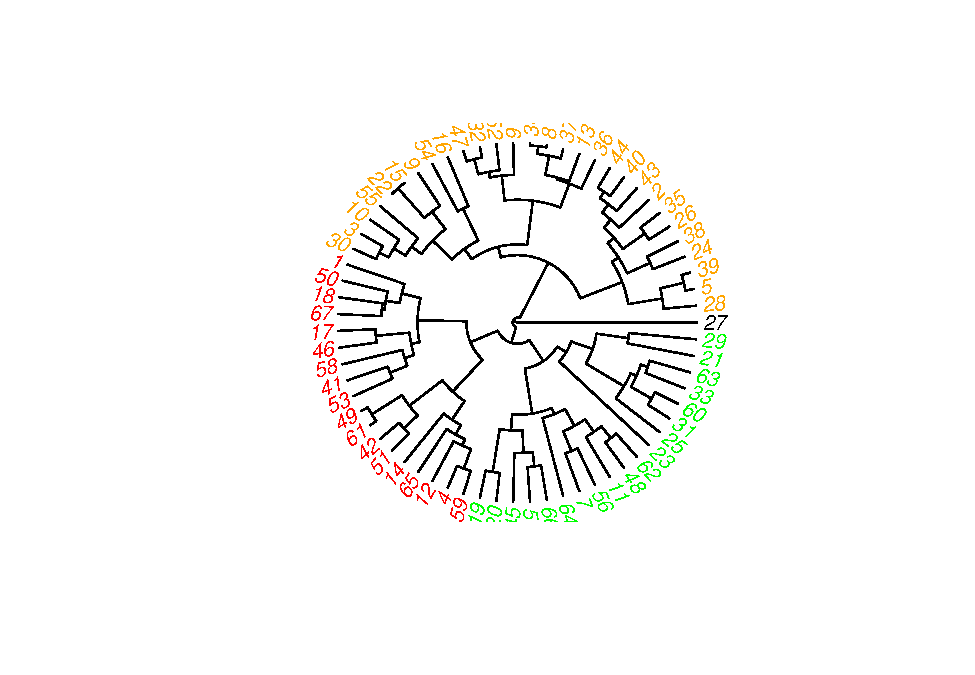
\includegraphics{codigo_files/figure-latex/creacion_clusters_dendrograma_centradoEscalado-1.pdf}

Lo exportamos a PDF tras la creación:

\begin{Shaded}
\begin{Highlighting}[]
\KeywordTok{pdf}\NormalTok{(}\StringTok{"Imágenes Obtenidas/dendrograma_pacientes_centscal.pdf"}\NormalTok{)}

\KeywordTok{plot}\NormalTok{(}\KeywordTok{as.phylo}\NormalTok{(hier.clust), }\DataTypeTok{type =} \StringTok{"fan"}\NormalTok{, }\DataTypeTok{tip.color =}\NormalTok{ colores.dendrograma[cluster.}\DecValTok{4}\NormalTok{], }\DataTypeTok{label.offset =} \FloatTok{0.3}\NormalTok{, }\DataTypeTok{cex =} \FloatTok{0.8}\NormalTok{)}

\KeywordTok{dev.off}\NormalTok{()}
\end{Highlighting}
\end{Shaded}

\begin{verbatim}
## pdf 
##   2
\end{verbatim}

Si lo comparamos, vemos que hemos obtenido exactamente el mismo
resultado, por lo que en este caso el centrado y escalado no es
necesario.

\subsection{K-Means}\label{k-means}

El algoritmo KMeans en principio no es el algoritmo más adecuado para
este trabajo, ya que se basa en círculos para la clasificación de los
individuos, cuando en principio en mis datos esto no es así. De todas
formas, voy a clasificar a los pacientes siguiendo este algoritmo para
comprobar la eficacia que tiene sobre mi problema:

Hacemos el clustering y vemos algunos resultados:

\begin{Shaded}
\begin{Highlighting}[]
\KeywordTok{set.seed}\NormalTok{(}\DecValTok{7}\NormalTok{)}

\NormalTok{datos.kmeans <-}\StringTok{ }\NormalTok{matriz.pacientes.datos }\CommentTok{# Sin la clasificación dentro del dataset}

\NormalTok{clusters <-}\StringTok{ }\KeywordTok{kmeans}\NormalTok{(datos.kmeans, }\DataTypeTok{centers=}\DecValTok{4}\NormalTok{)}
\NormalTok{clusters}\OperatorTok{$}\NormalTok{centers}
\end{Highlighting}
\end{Shaded}

\begin{verbatim}
##       edad       sex rel_ctxo_rel_mala rel_ctxo_trauma rel_ctxo_buena    ed_perm   ed_norm
## 1 23.82609 0.1739130        0.08695652       0.3043478      0.6086957 0.08695652 0.6956522
## 2 16.61111 0.2777778        0.05555556       0.3888889      0.5555556 0.61111111 0.1666667
## 3 30.94118 0.1176471        0.17647059       0.3529412      0.4705882 0.11764706 0.6470588
## 4 44.44444 0.3333333        0.33333333       0.4444444      0.2222222 0.44444444 0.3333333
##     ed_estr  resil_ba   resil_me  resil_al   pen_dic    gen_ex      etiq   fil_men   max_min
## 1 0.2173913 0.4782609 0.52173913 0.0000000 0.9130435 0.9565217 1.0000000 0.7826087 0.9565217
## 2 0.2222222 0.9444444 0.05555556 0.0000000 0.8333333 0.9444444 0.7777778 0.7222222 0.9444444
## 3 0.2352941 0.4705882 0.52941176 0.0000000 0.9411765 1.0000000 0.5882353 0.8235294 1.0000000
## 4 0.2222222 0.2222222 0.66666667 0.1111111 0.8888889 0.8888889 0.3333333 0.8888889 1.0000000
##    conc_arb  pseu_res       deb   raz_emo     inhib      asert     agres    impuls
## 1 1.0000000 0.6956522 1.0000000 0.9130435 0.7826087 0.08695652 0.1304348 0.5652174
## 2 0.9444444 0.2222222 0.7777778 0.8333333 0.6666667 0.00000000 0.3333333 0.5000000
## 3 1.0000000 0.6470588 1.0000000 0.7058824 0.5294118 0.23529412 0.2352941 0.7647059
## 4 1.0000000 0.3333333 1.0000000 0.5555556 0.5555556 0.33333333 0.1111111 0.6666667
\end{verbatim}

\begin{Shaded}
\begin{Highlighting}[]
\NormalTok{prediccion.kmeans <-}\StringTok{ }\NormalTok{clusters}\OperatorTok{$}\NormalTok{cluster}
\NormalTok{prediccion.kmeans}
\end{Highlighting}
\end{Shaded}

\begin{verbatim}
##  [1] 2 2 1 2 1 1 1 1 1 2 3 2 1 2 2 2 4 1 1 1 1 2 4 1 4 2 2 1 4 2 3 1 3 1 2 1 2 3 3 3 3 1 1 2 4 4 3 1
## [49] 3 3 3 3 4 2 2 4 3 3 2 1 1 3 3 1 3 4 1
\end{verbatim}

Interpretando estos resultados, obtenemos:

\begin{itemize}
\item
  El cluster 1 destaca por sexo más hacia masculino que otros, una
  relación contexto ciertamente buena, una educación permisiva, una
  resiliencia baja, maximización y minimización, razonamiento emocional,
  cierta inhibición y poca agresividad.
\item
  El cluster 2 destaca por una edad mayor, es el cluster con mejor
  relación con el contexto, y suelen tener las personas de este cluster
  una educación normal. Destaca por una resiliencia media, pensamiento
  dicotómico, generalización excesiva, etiquetado, conclusiones
  arbitrarias, deberías, razonamiento emocional e inhibición.
\item
  El cluster número 3 destaca por tener una edad aún más elevada, más
  ratio de personas del sexo femenino que ningún otro cluster, y tienen
  una relación con el contexto bastante variable. La educación de estas
  personas es principalmente normal, con una resiliencia que puede ser
  tanto baja como media. Destacan por el pensamiento dicotómico,
  generalización excesiva, poco etiquetado, maximización y minimización,
  filtro mental, conclusiones arbitrarias, pseudoresponsabilidad,
  deberías, y suelen ser bastante inhibidos e impulsivos.
\item
  Finalmente, el cluster 4 destaca por ser el que tiene la edad más
  elevada y el ratio de sexo más masculino. La relación con el contexto
  de estos individuos clasificados en este grupo es principalmente de
  trauma, aunque también hay buenas y malas. La educación de estos
  individuos es principalmente permisiva, y la resiliciencia tiende a
  media. Destacan por la poca etiquetación que hacen, pero un gran fitro
  mental, conclusiones arbitrarias, poca pseudo-responsabilidad, muchos
  deberías, poco razonamiento emocional, y son principalmente inhibidos
  e impulsivos.
\end{itemize}

Ahora sacamos la gráfica para poder ver como los ha clasificado sobre
dos componentes principales artificiales:

\begin{Shaded}
\begin{Highlighting}[]
\CommentTok{# Representado sobre las dos componentes principales que más explicación nos dan de las variables}

\KeywordTok{clusplot}\NormalTok{(datos.kmeans, clusters}\OperatorTok{$}\NormalTok{cluster, }\DataTypeTok{color =} \OtherTok{TRUE}\NormalTok{, }\DataTypeTok{main =} \StringTok{"Representación 2D con Clusplot"}\NormalTok{, }\DataTypeTok{labels =} \DecValTok{4}\NormalTok{, }\DataTypeTok{xlab =} \StringTok{"Comp 1"}\NormalTok{, }\DataTypeTok{ylab =} \StringTok{"Comp 2"}\NormalTok{) }
\end{Highlighting}
\end{Shaded}

\includegraphics{codigo_files/figure-latex/plots_k-means-1.pdf}

\begin{Shaded}
\begin{Highlighting}[]
\CommentTok{# Ahora la siguiente representación será con componentes discriminantes, que son las dos dimensiones sobre las que la representación de datos es más linealmente separable respecto a la predicción de grupos que ha hecho KMeans}

\KeywordTok{plotcluster}\NormalTok{(datos.kmeans, clusters}\OperatorTok{$}\NormalTok{cluster)}
\end{Highlighting}
\end{Shaded}

\includegraphics{codigo_files/figure-latex/plots_k-means-2.pdf}

Exportamos a PDF los gráficos obtenidos del KMeans:

\begin{Shaded}
\begin{Highlighting}[]
\KeywordTok{pdf}\NormalTok{(}\StringTok{"Imágenes Obtenidas/ResultadosKmeans.pdf"}\NormalTok{)}

\KeywordTok{clusplot}\NormalTok{(datos.kmeans, clusters}\OperatorTok{$}\NormalTok{cluster, }\DataTypeTok{color =} \OtherTok{TRUE}\NormalTok{, }\DataTypeTok{main =} \StringTok{"Representación 2D con Clusplot"}\NormalTok{, }\DataTypeTok{labels =} \DecValTok{4}\NormalTok{, }\DataTypeTok{xlab =} \StringTok{"Comp 1"}\NormalTok{, }\DataTypeTok{ylab =} \StringTok{"Comp 2"}\NormalTok{) }
\KeywordTok{plotcluster}\NormalTok{(datos.kmeans, clusters}\OperatorTok{$}\NormalTok{cluster)}

\NormalTok{dev.off}
\end{Highlighting}
\end{Shaded}

\begin{verbatim}
## function (which = dev.cur()) 
## {
##     if (which == 1) 
##         stop("cannot shut down device 1 (the null device)")
##     .External(C_devoff, as.integer(which))
##     dev.cur()
## }
## <bytecode: 0x0000000015754360>
## <environment: namespace:grDevices>
\end{verbatim}

\subsection{Minería de Reglas - Rules}\label{mineria-de-reglas---rules}

Para esto usaremos la librería RWeka, que es la implementación en R de
Weka. Como matriz de inicio, usaremos la matriz.pacientes.datos, que
está ya limpia.

\subsubsection{Reglas de Sexo}\label{reglas-de-sexo}

\begin{Shaded}
\begin{Highlighting}[]
\CommentTok{# Lo primero que tengo que hacer es convertir el sexo en un factor si no lo es}

\NormalTok{matriz.pacientes.datos.rm =}\StringTok{ }\NormalTok{matriz.pacientes.datos}

\NormalTok{matriz.pacientes.datos.rm}\OperatorTok{$}\NormalTok{sex <-}\StringTok{ }\KeywordTok{as.factor}\NormalTok{(matriz.pacientes.datos.rm}\OperatorTok{$}\NormalTok{sex)}

\NormalTok{part_sex <-}\StringTok{ }\KeywordTok{PART}\NormalTok{(sex}\OperatorTok{~}\NormalTok{., }\DataTypeTok{data =}\NormalTok{ matriz.pacientes.datos.rm)}
\NormalTok{oneR_sex <-}\StringTok{ }\KeywordTok{OneR}\NormalTok{(sex}\OperatorTok{~}\NormalTok{., }\DataTypeTok{data =}\NormalTok{ matriz.pacientes.datos.rm)}
\NormalTok{jrip_sex <-}\StringTok{ }\KeywordTok{JRip}\NormalTok{(sex}\OperatorTok{~}\NormalTok{., }\DataTypeTok{data =}\NormalTok{ matriz.pacientes.datos.rm)}

\KeywordTok{print}\NormalTok{(}\StringTok{"Reglas sexo PART"}\NormalTok{)}
\end{Highlighting}
\end{Shaded}

\begin{verbatim}
## [1] "Reglas sexo PART"
\end{verbatim}

\begin{Shaded}
\begin{Highlighting}[]
\NormalTok{part_sex}
\end{Highlighting}
\end{Shaded}

\begin{verbatim}
## PART decision list
## ------------------
## 
## agres <= 0 AND
## pen_dic > 0 AND
## rel_ctxo_trauma <= 0: 0 (34.0/4.0)
## 
## gen_ex > 0 AND
## pen_dic > 0 AND
## ed_estr <= 0 AND
## edad <= 32 AND
## impuls > 0 AND
## raz_emo > 0 AND
## edad > 15: 0 (9.0/2.0)
## 
## gen_ex > 0 AND
## agres <= 0 AND
## ed_norm <= 0: 0 (8.0)
## 
## gen_ex > 0 AND
## pen_dic > 0 AND
## pseu_res <= 0: 1 (6.0/1.0)
## 
## resil_ba <= 0: 0 (8.0/1.0)
## 
## : 1 (2.0)
## 
## Number of Rules  :   6
\end{verbatim}

\begin{Shaded}
\begin{Highlighting}[]
\KeywordTok{print}\NormalTok{(}\StringTok{"Regla sexo OneR"}\NormalTok{)}
\end{Highlighting}
\end{Shaded}

\begin{verbatim}
## [1] "Regla sexo OneR"
\end{verbatim}

\begin{Shaded}
\begin{Highlighting}[]
\NormalTok{oneR_sex}
\end{Highlighting}
\end{Shaded}

\begin{verbatim}
## edad:
##  < 49.5  -> 0
##  >= 49.5 -> 1
## (54/67 instances correct)
\end{verbatim}

\begin{Shaded}
\begin{Highlighting}[]
\KeywordTok{print}\NormalTok{(}\StringTok{"Reglas sexo JRip"}\NormalTok{)}
\end{Highlighting}
\end{Shaded}

\begin{verbatim}
## [1] "Reglas sexo JRip"
\end{verbatim}

\begin{Shaded}
\begin{Highlighting}[]
\NormalTok{jrip_sex}
\end{Highlighting}
\end{Shaded}

\begin{verbatim}
## JRIP rules:
## ===========
## 
##  => sex=0 (67.0/14.0)
## 
## Number of Rules : 1
\end{verbatim}

Como podemos ver, del sexo no podemos sacar ninguna regla demasiado
fiable, por lo que no podemos predecirlo demasiado bien.

\subsubsection{Reglas de impulsividad}\label{reglas-de-impulsividad}

\begin{Shaded}
\begin{Highlighting}[]
\CommentTok{# Lo primero que tengo que hacer es convertir el sexo en un factor si no lo es}

\NormalTok{matriz.pacientes.datos.rm =}\StringTok{ }\NormalTok{matriz.pacientes.datos}

\NormalTok{matriz.pacientes.datos.rm}\OperatorTok{$}\NormalTok{impuls <-}\StringTok{ }\KeywordTok{as.factor}\NormalTok{(matriz.pacientes.datos.rm}\OperatorTok{$}\NormalTok{impuls)}

\NormalTok{part_imp <-}\StringTok{ }\KeywordTok{PART}\NormalTok{(impuls}\OperatorTok{~}\NormalTok{., }\DataTypeTok{data =}\NormalTok{ matriz.pacientes.datos.rm)}
\NormalTok{oneR_imp <-}\StringTok{ }\KeywordTok{OneR}\NormalTok{(impuls}\OperatorTok{~}\NormalTok{., }\DataTypeTok{data =}\NormalTok{ matriz.pacientes.datos.rm)}
\NormalTok{jrip_imp <-}\StringTok{ }\KeywordTok{JRip}\NormalTok{(impuls}\OperatorTok{~}\NormalTok{., }\DataTypeTok{data =}\NormalTok{ matriz.pacientes.datos.rm)}

\KeywordTok{print}\NormalTok{(}\StringTok{"Reglas impulsividad PART"}\NormalTok{)}
\end{Highlighting}
\end{Shaded}

\begin{verbatim}
## [1] "Reglas impulsividad PART"
\end{verbatim}

\begin{Shaded}
\begin{Highlighting}[]
\NormalTok{part_imp}
\end{Highlighting}
\end{Shaded}

\begin{verbatim}
## PART decision list
## ------------------
## 
## agres > 0: 1 (14.0)
## 
## rel_ctxo_rel_mala <= 0 AND
## pen_dic > 0 AND
## ed_perm > 0: 0 (7.0/1.0)
## 
## pen_dic > 0 AND
## rel_ctxo_rel_mala > 0: 1 (6.0)
## 
## pen_dic <= 0: 0 (5.0)
## 
## sex > 0 AND
## pseu_res <= 0: 0 (3.0)
## 
## rel_ctxo_trauma <= 0 AND
## etiq > 0 AND
## inhib > 0 AND
## pseu_res <= 0: 1 (8.0/1.0)
## 
## rel_ctxo_trauma > 0: 1 (8.0/1.0)
## 
## etiq > 0 AND
## inhib > 0 AND
## edad <= 26: 0 (7.0)
## 
## etiq > 0: 1 (7.0/1.0)
## 
## : 0 (2.0)
## 
## Number of Rules  :   10
\end{verbatim}

\begin{Shaded}
\begin{Highlighting}[]
\KeywordTok{print}\NormalTok{(}\StringTok{"Regla impulsividad OneR"}\NormalTok{)}
\end{Highlighting}
\end{Shaded}

\begin{verbatim}
## [1] "Regla impulsividad OneR"
\end{verbatim}

\begin{Shaded}
\begin{Highlighting}[]
\NormalTok{oneR_imp}
\end{Highlighting}
\end{Shaded}

\begin{verbatim}
## edad:
##  < 22.5  -> 1
##  < 25.5  -> 0
##  < 46.0  -> 1
##  >= 46.0 -> 0
## (46/67 instances correct)
\end{verbatim}

\begin{Shaded}
\begin{Highlighting}[]
\KeywordTok{print}\NormalTok{(}\StringTok{"Reglas impulsividad JRip"}\NormalTok{)}
\end{Highlighting}
\end{Shaded}

\begin{verbatim}
## [1] "Reglas impulsividad JRip"
\end{verbatim}

\begin{Shaded}
\begin{Highlighting}[]
\NormalTok{jrip_imp}
\end{Highlighting}
\end{Shaded}

\begin{verbatim}
## JRIP rules:
## ===========
## 
## (agres <= 0) and (edad <= 25) => impuls=0 (29.0/10.0)
##  => impuls=1 (38.0/7.0)
## 
## Number of Rules : 2
\end{verbatim}

De la impulsividad vemos que es un poco más predecible, pero tampoco
obtenemos numerosas reglas generales.

\subsubsection{Reglas de agresividad}\label{reglas-de-agresividad}

\begin{Shaded}
\begin{Highlighting}[]
\CommentTok{# Lo primero que tengo que hacer es convertir el sexo en un factor si no lo es}

\NormalTok{matriz.pacientes.datos.rm =}\StringTok{ }\NormalTok{matriz.pacientes.datos}

\NormalTok{matriz.pacientes.datos.rm}\OperatorTok{$}\NormalTok{agres <-}\StringTok{ }\KeywordTok{as.factor}\NormalTok{(matriz.pacientes.datos.rm}\OperatorTok{$}\NormalTok{agres)}

\NormalTok{part_agr <-}\StringTok{ }\KeywordTok{PART}\NormalTok{(agres}\OperatorTok{~}\NormalTok{., }\DataTypeTok{data =}\NormalTok{ matriz.pacientes.datos.rm)}
\NormalTok{oneR_agr <-}\StringTok{ }\KeywordTok{OneR}\NormalTok{(agres}\OperatorTok{~}\NormalTok{., }\DataTypeTok{data =}\NormalTok{ matriz.pacientes.datos.rm)}
\NormalTok{jrip_agr <-}\StringTok{ }\KeywordTok{JRip}\NormalTok{(agres}\OperatorTok{~}\NormalTok{., }\DataTypeTok{data =}\NormalTok{ matriz.pacientes.datos.rm)}

\KeywordTok{print}\NormalTok{(}\StringTok{"Reglas agresividad PART"}\NormalTok{)}
\end{Highlighting}
\end{Shaded}

\begin{verbatim}
## [1] "Reglas agresividad PART"
\end{verbatim}

\begin{Shaded}
\begin{Highlighting}[]
\NormalTok{part_agr}
\end{Highlighting}
\end{Shaded}

\begin{verbatim}
## PART decision list
## ------------------
## 
## inhib > 0: 0 (44.0)
## 
## asert <= 0: 1 (14.0/1.0)
## 
## : 0 (9.0/1.0)
## 
## Number of Rules  :   3
\end{verbatim}

\begin{Shaded}
\begin{Highlighting}[]
\KeywordTok{print}\NormalTok{(}\StringTok{"Regla Agresividad OneR"}\NormalTok{)}
\end{Highlighting}
\end{Shaded}

\begin{verbatim}
## [1] "Regla Agresividad OneR"
\end{verbatim}

\begin{Shaded}
\begin{Highlighting}[]
\NormalTok{oneR_agr}
\end{Highlighting}
\end{Shaded}

\begin{verbatim}
## inhib:
##  < 0.5   -> 1
##  >= 0.5  -> 0
## (58/67 instances correct)
\end{verbatim}

\begin{Shaded}
\begin{Highlighting}[]
\KeywordTok{print}\NormalTok{(}\StringTok{"Reglas agresividad JRip"}\NormalTok{)}
\end{Highlighting}
\end{Shaded}

\begin{verbatim}
## [1] "Reglas agresividad JRip"
\end{verbatim}

\begin{Shaded}
\begin{Highlighting}[]
\NormalTok{jrip_agr}
\end{Highlighting}
\end{Shaded}

\begin{verbatim}
## JRIP rules:
## ===========
## 
## (inhib <= 0) and (asert <= 0) => agres=1 (14.0/1.0)
##  => agres=0 (53.0/1.0)
## 
## Number of Rules : 2
\end{verbatim}

\subsubsection{Reglas de grupo}\label{reglas-de-grupo}

Las más importantes:

\begin{Shaded}
\begin{Highlighting}[]
\CommentTok{# Lo primero que tengo que hacer es convertir el sexo en un factor si no lo es}

\NormalTok{matriz.pacientes.datos.rm =}\StringTok{ }\NormalTok{matriz.pacientes.datos}
\NormalTok{matriz.pacientes.datos.rm <-}\StringTok{ }\KeywordTok{cbind}\NormalTok{(matriz.pacientes.datos.rm, dataset}\OperatorTok{$}\NormalTok{grupo)}

\NormalTok{matriz.pacientes.datos.rm}\OperatorTok{$}\StringTok{`}\DataTypeTok{dataset$grupo}\StringTok{`}\NormalTok{ <-}\StringTok{ }\KeywordTok{as.factor}\NormalTok{(matriz.pacientes.datos.rm}\OperatorTok{$}\StringTok{`}\DataTypeTok{dataset$grupo}\StringTok{`}\NormalTok{)}

\NormalTok{part_gru <-}\StringTok{ }\KeywordTok{PART}\NormalTok{(}\StringTok{`}\DataTypeTok{dataset$grupo}\StringTok{`}\OperatorTok{~}\NormalTok{., }\DataTypeTok{data =}\NormalTok{ matriz.pacientes.datos.rm)}
\NormalTok{oneR_gru <-}\StringTok{ }\KeywordTok{OneR}\NormalTok{(}\StringTok{`}\DataTypeTok{dataset$grupo}\StringTok{`}\OperatorTok{~}\NormalTok{., }\DataTypeTok{data =}\NormalTok{ matriz.pacientes.datos.rm)}
\NormalTok{jrip_gru <-}\StringTok{ }\KeywordTok{JRip}\NormalTok{(}\StringTok{`}\DataTypeTok{dataset$grupo}\StringTok{`}\OperatorTok{~}\NormalTok{., }\DataTypeTok{data =}\NormalTok{ matriz.pacientes.datos.rm)}

\KeywordTok{print}\NormalTok{(}\StringTok{"Reglas grupo PART"}\NormalTok{)}
\end{Highlighting}
\end{Shaded}

\begin{verbatim}
## [1] "Reglas grupo PART"
\end{verbatim}

\begin{Shaded}
\begin{Highlighting}[]
\NormalTok{part_gru}
\end{Highlighting}
\end{Shaded}

\begin{verbatim}
## PART decision list
## ------------------
## 
## impuls <= 0 AND
## fil_men > 0 AND
## pen_dic > 0 AND
## resil_me <= 0 AND
## rel_ctxo_trauma <= 0: 2 (9.0/3.0)
## 
## impuls <= 0 AND
## fil_men <= 0: 2 (6.0)
## 
## impuls <= 0 AND
## resil_ba <= 0 AND
## pseu_res <= 0: 2 (4.0)
## 
## impuls <= 0 AND
## ed_estr <= 0: 3 (5.0/1.0)
## 
## impuls > 0 AND
## deb > 0 AND
## resil_ba <= 0 AND
## ed_estr <= 0 AND
## sex <= 0 AND
## ed_perm <= 0 AND
## pseu_res > 0: 2 (6.0)
## 
## impuls > 0 AND
## gen_ex > 0 AND
## etiq > 0 AND
## fil_men > 0 AND
## rel_ctxo_rel_mala <= 0 AND
## pseu_res > 0 AND
## rel_ctxo_trauma <= 0: 1 (5.0/1.0)
## 
## impuls > 0 AND
## gen_ex > 0 AND
## etiq > 0 AND
## fil_men <= 0: 4 (3.0)
## 
## impuls > 0 AND
## fil_men <= 0: 1 (3.0/1.0)
## 
## impuls <= 0: 2 (2.0)
## 
## rel_ctxo_rel_mala > 0 AND
## edad <= 37: 1 (2.0)
## 
## rel_ctxo_rel_mala <= 0 AND
## max_min > 0 AND
## raz_emo > 0 AND
## inhib > 0: 4 (6.0/3.0)
## 
## rel_ctxo_rel_mala <= 0 AND
## rel_ctxo_trauma > 0 AND
## ed_norm <= 0: 4 (7.0/2.0)
## 
## rel_ctxo_rel_mala <= 0 AND
## raz_emo > 0: 2 (4.0/1.0)
## 
## rel_ctxo_rel_mala <= 0: 1 (3.0/1.0)
## 
## : 2 (2.0)
## 
## Number of Rules  :   15
\end{verbatim}

\begin{Shaded}
\begin{Highlighting}[]
\KeywordTok{print}\NormalTok{(}\StringTok{"Regla grupo OneR"}\NormalTok{)}
\end{Highlighting}
\end{Shaded}

\begin{verbatim}
## [1] "Regla grupo OneR"
\end{verbatim}

\begin{Shaded}
\begin{Highlighting}[]
\NormalTok{oneR_gru}
\end{Highlighting}
\end{Shaded}

\begin{verbatim}
## agres:
##  < 0.5   -> 2
##  >= 0.5  -> 1
## (32/67 instances correct)
\end{verbatim}

\begin{Shaded}
\begin{Highlighting}[]
\KeywordTok{print}\NormalTok{(}\StringTok{"Reglas grupo JRip"}\NormalTok{)}
\end{Highlighting}
\end{Shaded}

\begin{verbatim}
## [1] "Reglas grupo JRip"
\end{verbatim}

\begin{Shaded}
\begin{Highlighting}[]
\NormalTok{jrip_gru}
\end{Highlighting}
\end{Shaded}

\begin{verbatim}
## JRIP rules:
## ===========
## 
## (edad >= 37) and (pseu_res >= 1) => dataset$grupo=1 (4.0/0.0)
##  => dataset$grupo=2 (63.0/33.0)
## 
## Number of Rules : 2
\end{verbatim}


\end{document}
